% !TEX program = xelatex
\documentclass[12pt,a4paper]{report}
\AtBeginDocument{\fontsize{13}{15.6}\selectfont} % 13pt body; report has no 13pt option
\usepackage{fontspec}
\setmainfont{Times New Roman}
\usepackage[english,main=vietnamese]{babel}
\usepackage[top=2cm,bottom=2cm,left=3cm,right=2cm]{geometry}
\usepackage{setspace}\onehalfspacing
\usepackage{graphicx,booktabs,amsmath,longtable,hyperref,caption,array}
\newcolumntype{L}[1]{>{\raggedright\arraybackslash}p{#1}} % cột văn bản hẹp: căn trái, tránh giãn chữ
\usepackage{placeins} % \FloatBarrier: giữ ảnh trong đúng mục (ch4_demo)
\usepackage{csquotes}
\usepackage[table]{xcolor}
\usepackage[style=apa,backend=biber,language=english,autolang=other,sortlocale=en_US]{biblatex} % biber has no Vietnamese locale
\DeclareLanguageMapping{english}{english-apa}
\addbibresource{references.bib}
% biblatex-apa has no vietnamese-apa.lbx: reuse the English APA strings for Vietnamese text
\DeclareLanguageMapping{vietnamese}{english-apa}
\hypersetup{hidelinks}
\graphicspath{{images/}}
\usepackage{tikz}\usetikzlibrary{arrows.meta,positioning,fit}

\begin{document}
% ---------- Bìa đồ án môn học (nền theo mẫu KL01, Khoa HTTT, UEL) ----------
% Ảnh nền (khung, logo, dải xanh) trích từ file hướng dẫn .doc của khoa.
\newcommand{\coverpage}{%
\begin{titlepage}
\begin{tikzpicture}[remember picture,overlay]
  \node[inner sep=0] at (current page.center)
    {
\includegraphics[width=\paperwidth,height=\paperheight]{cover-kl01-vi}};
  \node[font=\bfseries\fontsize{16}{20}\selectfont] at ([yshift=-4.6cm]current page.north) {KHOA HỆ THỐNG THÔNG TIN};
  \node[font=\bfseries\fontsize{12}{15}\selectfont,align=center] at ([yshift=-11.4cm]current page.north)
    {Học kỳ I/2026 -- 2027\\[0.3cm]ĐỒ ÁN MÔN HỌC: HỌC MÁY TRONG PHÂN TÍCH KINH DOANH};
  % Tiêu đề: neo đỉnh (anchor=north) để không đè lên dòng môn học; phụ đề ngắt 3 dòng cân nhau.
  \node[font=\bfseries\fontsize{18}{24}\selectfont,text width=16cm,align=center,anchor=north]
    at ([yshift=-12.3cm]current page.north)
    {GIAO ĐÚNG HẠN, VẪN CHƯA HÀI LÒNG\\[8pt]
     {\fontsize{14}{20}\selectfont HỆ THỐNG HỌC MÁY PHÁT HIỆN SỚM VÀ\\
      ƯU TIÊN CHĂM SÓC ĐƠN HÀNG CÓ NGUY CƠ\\
      BẤT MÃN ẨN TRÊN DỮ LIỆU OLIST}};
  \node[font=\bfseries\fontsize{13}{18}\selectfont,anchor=north west,align=left]
    at ([xshift=-3.2cm,yshift=-17.7cm]current page.north)
    {GVHD: TS. Trần Duy Thanh\\[6pt]
     Nhóm sinh viên thực hiện:\\[2pt]
     {\fontsize{12}{16}\selectfont\begin{tabular}{@{}ll@{}}
       K244161784 & Nguyễn Trần Thái Huy\\
       K244161819 & Vũ Sơn Trúc\\
       K244161818 & Nguyễn Minh Trung\\
       K244161803 & Vòng Hữu Quân\\
       K244161779 & Vũ Anh Đào
     \end{tabular}}};
  \node[font=\bfseries\fontsize{13}{16}\selectfont,text=white]
    at ([yshift=2.25cm]current page.south) {TP.HCM, THÁNG \,11/2026};
\end{tikzpicture}
\end{titlepage}}
\coverpage   % trang bìa

\pagenumbering{roman}
% Thứ tự theo hướng dẫn Khoa HTTT, mục II
% Lời cảm ơn và lời cam kết (theo thứ tự hướng dẫn Khoa HTTT).
\chapter*{Lời cảm ơn}
\addcontentsline{toc}{chapter}{Lời cảm ơn}

Trước hết, nhóm xin gửi lời cảm ơn chân thành đến TS.~Trần Duy Thanh, giảng viên hướng dẫn, đã tận tình định hướng đồ án, góp ý về phương pháp và dành thời gian theo sát nhóm trong suốt quá trình thực hiện đồ án. Những nhận xét của Thầy giúp nhóm xác định rõ phạm vi bài toán, chú trọng tính chặt chẽ của thiết kế thực nghiệm và trình bày kết quả một cách trung thực.

Nhóm cũng xin cảm ơn quý Thầy Cô Khoa Hệ thống Thông tin, Trường Đại học Kinh tế -- Luật, Đại học Quốc gia Thành phố Hồ Chí Minh, đã truyền đạt nền tảng kiến thức về phân tích dữ liệu, học máy và phát triển hệ thống thông tin, là cơ sở để nhóm hoàn thành đồ án này.

Nhóm trân trọng cảm ơn Olist đã công bố bộ dữ liệu \emph{Brazilian E-Commerce Public Dataset}, cùng cộng đồng phát triển các công cụ mã nguồn mở mà nhóm sử dụng trong quá trình xây dựng kho dữ liệu, huấn luyện mô hình và phát triển ứng dụng.

Cuối cùng, nhóm xin cảm ơn gia đình và bạn bè đã luôn động viên, hỗ trợ trong thời gian thực hiện đồ án. Dù đã nỗ lực hoàn thiện, đồ án khó tránh khỏi thiếu sót; nhóm rất mong nhận được ý kiến đóng góp của quý Thầy Cô để đồ án được hoàn thiện hơn.

\vspace{1cm}
\begin{flushright}
\begin{minipage}{0.5\linewidth}\centering
TP.HCM, ngày 16 tháng 11 năm 2026\\
\textbf{Nhóm sinh viên thực hiện}
\end{minipage}
\end{flushright}

\chapter*{Lời cam kết}
\addcontentsline{toc}{chapter}{Lời cam kết}

Nhóm sinh viên thực hiện xin cam kết đồ án môn học Học máy trong phân tích kinh doanh ``Giao đúng hạn, vẫn chưa hài lòng: Hệ thống học máy phát hiện sớm và ưu tiên chăm sóc đơn hàng có nguy cơ bất mãn ẩn trên dữ liệu Olist'' là công trình nghiên cứu của nhóm, được thực hiện dưới sự hướng dẫn của TS.~Trần Duy Thanh.

Các số liệu và kết quả trình bày trong đồ án được tạo ra từ quá trình xử lý dữ liệu và thực nghiệm của nhóm trên bộ dữ liệu công khai của Olist, có thể truy vết về cấu hình thí nghiệm và mã nguồn tương ứng. Nhóm không sao chép kết quả của công trình khác. Các tài liệu, số liệu và ý tưởng tham khảo từ nghiên cứu trước đều được trích dẫn đầy đủ và ghi rõ nguồn trong danh mục tài liệu tham khảo.

Nhóm cũng cam kết trình bày trung thực phạm vi và giới hạn của kết quả: các chỉ số được báo cáo là kết quả phát triển trên các fold kiểm định theo thời gian, dữ liệu minh họa trong bản demo được ghi rõ là dữ liệu minh họa, và các kết luận mang tính dự báo, không phải kết luận nhân quả.

Nhóm xin hoàn toàn chịu trách nhiệm về nội dung của đồ án này.

\clearpage
\vspace{1cm}
\begin{center}
{\large\textbf{DANH SÁCH THÀNH VIÊN}}\\[0.8cm]
{\renewcommand{\arraystretch}{1.5}
\begin{tabular}{|c|>{\centering\arraybackslash}p{6cm}|c|>{\centering\arraybackslash}p{3.3cm}|}
\hline
\textbf{STT} & \textbf{HỌ VÀ TÊN} & \textbf{MSSV} & \textbf{MỨC ĐỘ ĐÓNG GÓP (\%)} \\
\hline
1 & Nguyễn Trần Thái Huy (Nhóm trưởng) & K244161784 & 100\% \\
\hline
2 & Nguyễn Minh Trung & K244161818 & 100\% \\
\hline
3 & Vòng Hữu Quân & K244161803 & 100\% \\
\hline
4 & Vũ Anh Đào & K244161779 & 100\% \\
\hline
5 & Vũ Sơn Trúc & K244161819 & 100\% \\
\hline
\end{tabular}}
\end{center}

\clearpage
\begin{table}[!htbp]
\centering
\caption{Phân công công việc của nhóm}\label{tab:team-assignment}
\scriptsize
\setlength{\tabcolsep}{3pt}
\renewcommand{\arraystretch}{1.05}
\begin{tabular}{@{}cL{2.8cm}L{5.5cm}L{5.5cm}@{}}
\toprule
\textbf{STT} & \textbf{Thành viên} & \textbf{Công việc dự án} & \textbf{Phân công viết báo cáo} \\
\midrule
1 & Nguyễn Trần Thái Huy &
Phụ trách chính phần lập trình, tích hợp kỹ thuật và học máy: xây dựng pipeline dữ liệu và mô hình theo thời gian; phát triển đặc trưng, huấn luyện, hiệu chỉnh, đánh giá và xuất mô hình; đồng thời trực tiếp phát triển, hoàn thiện nhiều thành phần backend và workflow xử lý case như hàng đợi rủi ro, nhận/giao đơn, liên hệ, đóng/mở lại case, dashboard, audit và tham số vận hành. Bên cạnh đó, phụ trách kiểm thử tự động, CI, dữ liệu demo, hardening phát hành và các lệnh vận hành toàn hệ thống. &
Viết toàn bộ Chương 3; cung cấp bảng chỉ số mô hình cho Chương 4; hỗ trợ tích hợp, chuẩn hóa và đối chiếu nội dung báo cáo với hệ thống đã triển khai. \\
\midrule
2 & Vũ Sơn Trúc &
Phụ trách giao diện, đồng thời hỗ trợ BA: xây dựng luồng người dùng và Figma; đặc tả API; phát triển các màn đăng nhập, dashboard, hàng đợi rủi ro, chi tiết đơn và lịch sử kiểm toán; bảo đảm hiển thị đa thiết bị và kết nối giao diện với API. &
Viết phần giao diện và demo của Chương 4; viết Chương 5 (Thảo luận). \\
\midrule
3 & Nguyễn Minh Trung &
Phụ trách backend và hỗ trợ điều phối kỹ thuật: xây dựng kiến trúc backend, các bảng Gold, API xác thực và phân quyền, Risk Queue, SLA, dashboard; đóng gói luồng dữ liệu, triển khai hệ thống và kiểm thử smoke test. &
Viết phần hệ thống và API của Chương 4; viết Chương 6 (Kết luận) và Phụ lục; ghép và rà soát bản báo cáo cuối. \\
\midrule
4 & Vòng Hữu Quân &
Phụ trách dữ liệu: EDA, nhãn và đặc trưng lịch sử; xây dựng luồng Bronze--Silver, bảng dữ liệu ứng dụng và dữ liệu demo; phát triển các API nhận, giao và xử lý đơn; hỗ trợ phân tích lỗi và các sơ đồ trình tự; thực hiện video demo hệ thống. &
Viết phần còn lại của Chương 2 (nghiên cứu liên quan và cơ sở lý thuyết); viết phần EDA và dữ liệu của Chương 4. \\
\midrule
5 & Vũ Anh Đào &
Phụ trách BA: xác định bài toán, phạm vi, tiêu chí thành công; xây dựng BRD, FRD, tiêu chí nghiệm thu và kịch bản kiểm thử; tham gia từ điển dữ liệu, ERD, kiến trúc hệ thống và kiểm thử đầu cuối. &
Viết Tóm tắt, Chương 1 (Giới thiệu) và mục 2.1 (các khái niệm liên quan); thiết kế slide báo cáo và thuyết trình. \\
\bottomrule
\end{tabular}
\end{table}
\clearpage

   % Lời cảm ơn, Lời cam kết
\tableofcontents
\listoffigures\addcontentsline{toc}{chapter}{Danh mục hình ảnh}
\listoftables\addcontentsline{toc}{chapter}{Danh mục bảng biểu}
% Danh mục từ viết tắt (đặt sau Danh mục bảng biểu theo hướng dẫn Khoa HTTT).
\chapter*{Danh mục từ viết tắt}
\addcontentsline{toc}{chapter}{Danh mục từ viết tắt}

\begin{longtable}{@{}p{3.2cm}p{11.5cm}@{}}
\toprule
\textbf{Từ viết tắt} & \textbf{Ý nghĩa} \\
\midrule
\endhead
\bottomrule
\endfoot
API     & Giao diện lập trình ứng dụng (\emph{Application Programming Interface}) \\
AP      & Độ chính xác trung bình (\emph{Average Precision}) \\
AUC     & Diện tích dưới đường cong (\emph{Area Under the Curve}) \\
CSKH    & Chăm sóc khách hàng \\
CSV     & Tệp dữ liệu phân tách bằng dấu phẩy (\emph{Comma-Separated Values}) \\
EDA     & Phân tích khám phá dữ liệu (\emph{Exploratory Data Analysis}) \\
F1      & Trung bình điều hòa của precision và recall \\
HHI     & Chỉ số Herfindahl--Hirschman \\
JWT     & Chuỗi xác thực dạng JSON (\emph{JSON Web Token}) \\
ML      & Học máy (\emph{Machine Learning}) \\
PR      & Precision--Recall \\
PR-AUC  & Diện tích dưới đường cong precision--recall \\
RF      & Rừng ngẫu nhiên (\emph{Random Forest}) \\
ROC     & Đường cong đặc tính hoạt động của bộ thu (\emph{Receiver Operating Characteristic}) \\
ROC-AUC & Diện tích dưới đường cong ROC \\
SHAP    & Giá trị giải thích dựa trên lý thuyết trò chơi (\emph{SHapley Additive exPlanations}) \\
SLA     & Cam kết thời hạn xử lý (\emph{Service Level Agreement}) \\
SMOTE   & Kỹ thuật sinh mẫu tổng hợp cho lớp thiểu số (\emph{Synthetic Minority Over-sampling Technique}) \\
SVM     & Máy vectơ hỗ trợ (\emph{Support Vector Machine}) \\
\end{longtable}
 \chapter*{Tóm tắt}

Trong thương mại điện tử, giao hàng trễ thường được xem là dấu hiệu rõ nhất cho thấy khách hàng có thể không hài lòng. Tuy nhiên, thực tế cho thấy nhiều đơn hàng vẫn được giao đúng hẹn nhưng nhận đánh giá thấp. Khách hàng có thể không hài lòng vì sản phẩm không đúng kỳ vọng, hàng bị thiếu hoặc hư hỏng, đơn có nhiều người bán nên giao nhận phức tạp, hoặc trải nghiệm mua hàng không tốt dù thời gian giao vẫn nằm trong cam kết. Đề tài gọi nhóm trường hợp này là ``bất mãn ẩn'' (\emph{hidden dissatisfaction}).

Xuất phát từ vấn đề trên, đề tài sử dụng bộ dữ liệu thương mại điện tử Olist để nghiên cứu khả năng nhận diện sớm những đơn hàng đã được giao đúng hạn nhưng có nguy cơ nhận đánh giá 1–2 sao. Thay vì chờ đến khi khách hàng để lại phản hồi tiêu cực, nhóm hướng đến việc tận dụng những thông tin đã có tại thời điểm giao hàng để dự báo rủi ro. Qua đó, kết quả nghiên cứu có thể hỗ trợ bộ phận chăm sóc khách hàng xác định những đơn cần được kiểm tra trước, đồng thời cung cấp thêm thông tin để cấp quản lý theo dõi tình hình và phân bổ nguồn lực phù hợp.

Để thực hiện mục tiêu này, nhóm xây dựng quy trình học máy dựa trên các thông tin của đơn hàng tại thời điểm giao hàng, chẳng hạn như sản phẩm được mua, người bán, giá trị đơn, phí vận chuyển, số lượng sản phẩm, số lượng người bán và quá trình xử lý đơn. Từ các thông tin này, mô hình ước lượng mức độ rủi ro của từng sản phẩm trong đơn, sau đó tổng hợp thành mức độ ưu tiên cho cả đơn hàng. Kết quả cuối cùng là một danh sách các đơn cần được xem xét trước thay vì xử lý toàn bộ đơn hàng theo cùng một thứ tự.

Ví dụ, một khách hàng đặt hai sản phẩm từ hai người bán khác nhau và đơn hàng vẫn được giao đúng hạn. Tuy nhiên, đơn có phí vận chuyển cao, nhiều bên cùng xử lý và một người bán có quá trình giao hàng thiếu ổn định. Dù chưa có đánh giá từ khách hàng, hệ thống có thể xếp đơn này vào nhóm cần theo dõi để nhân viên kiểm tra sớm hơn các đơn có rủi ro thấp.

Do dữ liệu Olist chỉ ghi nhận đánh giá ở cấp đơn hàng, đề tài không thể khẳng định sản phẩm nào là nguyên nhân trực tiếp khiến khách hàng không hài lòng. Vì vậy, kết quả của mô hình chỉ được sử dụng như một tín hiệu hỗ trợ ưu tiên, không phải kết luận về nguyên nhân hay căn cứ để tự động xử lý khách hàng.

Kết quả phát triển ban đầu của nhóm cho thấy mô hình có thể hỗ trợ xếp hạng các đơn có nguy cơ nhận đánh giá thấp tốt hơn cách lựa chọn ngẫu nhiên. Bên cạnh mô hình dự báo, đề tài xây dựng hệ thống hỗ trợ nhân viên theo dõi danh sách rủi ro, xem thông tin đơn hàng, phân công xử lý, ghi nhận quá trình liên hệ và lưu lại lịch sử thao tác. Đồng thời, cấp quản lý có thể theo dõi tình hình xử lý, thiết lập ngưỡng ưu tiên phù hợp với năng lực của đội ngũ, quản lý các tham số vận hành và xem lại lịch sử quyết định. Qua đó, hệ thống không chỉ hỗ trợ nhân viên xử lý từng trường hợp mà còn cung cấp thông tin để nhà quản lý phân bổ nguồn lực, giám sát chất lượng xử lý và đưa ra quyết định phù hợp hơn.

\par\medskip
\noindent\textbf{Từ khóa:} thương mại điện tử, sự hài lòng khách hàng, bất mãn ẩn, học máy, Olist, dự báo rủi ro.
 \addcontentsline{toc}{chapter}{Tóm tắt}  % tối đa 1 trang A4
\clearpage\pagenumbering{arabic}

\chapter{Giới thiệu}
\label{chap:gioi-thieu}

\section{Bối cảnh và lý do thực hiện đề tài}
\label{sec:boi-canh}

Trong những năm gần đây, thương mại điện tử ngày càng trở thành một hình thức mua sắm quen thuộc, mang đến cho khách hàng nhiều lựa chọn và sự thuận tiện trong quá trình đặt hàng. Tuy nhiên, khi người mua không thể trực tiếp kiểm tra sản phẩm trước khi nhận, trải nghiệm mua sắm không chỉ phụ thuộc vào chất lượng hàng hóa mà còn chịu ảnh hưởng từ nhiều yếu tố khác như thông tin sản phẩm, giá cả, phí vận chuyển, thời gian xử lý đơn hàng và chất lượng giao nhận. Vì vậy, đánh giá trực tuyến của khách hàng trở thành một nguồn thông tin quan trọng, giúp doanh nghiệp hiểu rõ hơn về chất lượng dịch vụ và những vấn đề phát sinh trong quá trình bán hàng. Nghiên cứu của (Deshpande \& Pendem, 2023) cũng cho thấy hiệu quả hoạt động logistics có mối liên hệ với điểm đánh giá, hành vi mua lại và doanh số của người bán trên các nền tảng thương mại điện tử. .

Trong số những yếu tố ảnh hưởng đến trải nghiệm khách hàng, thời gian giao hàng thường được quan tâm nhiều nhất. Giao hàng trễ thường là dấu hiệu rõ nhất của trải nghiệm không tốt. Khi đơn hàng đến muộn hơn thời gian đã cam kết, doanh nghiệp có thể dễ dàng đưa đơn đó vào nhóm cần kiểm tra. Tuy nhiên, giao đúng hẹn chưa đồng nghĩa với việc khách hàng hài lòng. Một đơn hàng vẫn có thể nhận đánh giá thấp nếu sản phẩm không đúng kỳ vọng, bị lỗi hoặc thiếu, nếu khách phải nhận nhiều kiện hàng vào những thời điểm khác nhau, hoặc nếu quá trình xử lý đơn tạo ra những bất tiện khác. Nghiên cứu của Ravula (2023) cho thấy khách hàng phản ứng tiêu cực rõ rệt với giao trễ; trong khi đó, Brylla và Walsh (2022) chỉ ra rằng việc giao nhanh nhưng tách đơn thành nhiều đợt vẫn có thể làm giảm sự hài lòng vì gây phiền toái cho người nhận.

Từ thực tế trên, có thể thấy rằng việc chỉ theo dõi các đơn hàng giao trễ chưa đủ để doanh nghiệp nhận diện toàn bộ những trải nghiệm không tốt của khách hàng. Những đơn hàng giao đúng hạn nhưng vẫn nhận đánh giá 1--2 sao là một nhóm đáng quan tâm. Đề tài gọi hiện tượng này là ``bất mãn ẩn'' (\emph{hidden dissatisfaction}). Sự bất mãn được gọi là ``ẩn'' vì nó không thể được phát hiện bằng cách chỉ theo dõi các đơn giao trễ. Nếu doanh nghiệp chỉ ưu tiên xử lý những đơn bị trễ, các trường hợp có nguy cơ đánh giá thấp do sản phẩm, người bán, cấu trúc đơn hàng hoặc các vấn đề khác sẽ dễ bị bỏ sót.

Xuất phát từ vấn đề đó, nhóm lựa chọn nghiên cứu khả năng ứng dụng học máy (Machine Learning) để nhận diện sớm những đơn hàng giao đúng hạn nhưng có nguy cơ nhận đánh giá thấp. Đề tài sử dụng bộ dữ liệu công khai \emph{Brazilian E-Commerce Public Dataset by Olist}. Bộ dữ liệu gồm thông tin về đơn hàng, sản phẩm, người bán, khách hàng, thanh toán, vận chuyển và đánh giá trong thị trường thương mại điện tử Brazil giai đoạn 2016--2018 (Olist, 2018). Với các nhóm thông tin có mối liên hệ với nhau, bộ dữ liệu này tạo điều kiện để nhóm tìm hiểu những tín hiệu có thể liên quan đến đánh giá của khách hàng, ngay cả khi đơn hàng đã được giao đúng hạn.

Thông qua nghiên cứu, nhóm hướng đến việc tận dụng dữ liệu sẵn có để hỗ trợ doanh nghiệp chuyển từ cách chăm sóc khách hàng mang tính phản ứng sang cách tiếp cận chủ động hơn. Thay vì chỉ xử lý khi khách hàng đã để lại đánh giá tiêu cực, hệ thống có thể giúp nhân viên xác định trước những đơn hàng cần được quan tâm, đồng thời cung cấp thêm thông tin để cấp quản lý theo dõi và phân bổ nguồn lực phù hợp.

\section{Vấn đề cần giải quyết}
\label{sec:van-de}

Từ bối cảnh đã trình bày, vấn đề mà đề tài tập trung giải quyết là làm thế nào để nhận diện những đơn hàng có nguy cơ nhận đánh giá thấp khi quá trình giao hàng vẫn diễn ra đúng thời gian dự kiến. Cụ thể, nhóm chỉ xem xét các đơn hàng đã được giao thành công, không muộn hơn ngày giao dự kiến và có đánh giá được tạo sau thời điểm giao hàng. Trong nhóm này, những đơn nhận đánh giá 1, 2 sao được xem là các trường hợp cần quan tâm.

Điểm quan trọng của bài toán là hệ thống không tìm cách xác định chính xác nguyên nhân khiến khách hàng không hài lòng. Thay vào đó, nhóm sử dụng những thông tin đã có tại thời điểm giao hàng để nhận diện các dấu hiệu rủi ro và sắp xếp những đơn cần được kiểm tra theo mức độ ưu tiên. Cách tiếp cận này phù hợp với thực tế khi bộ phận chăm sóc khách hàng có giới hạn về nhân sự và thời gian, không thể chủ động kiểm tra tất cả đơn hàng với cùng một mức độ quan tâm.

Để khai thác tốt hơn các thông tin trong bộ dữ liệu của Olist, mô hình được xây dựng ở cấp sản phẩm trong đơn hàng. Một đơn có thể chứa nhiều sản phẩm và do nhiều người bán cùng xử lý; vì vậy, việc xem xét từng sản phẩm giúp giữ lại các thông tin chi tiết về sản phẩm, người bán và cấu trúc đơn. Tuy nhiên, dữ liệu Olist chỉ ghi nhận đánh giá chung cho đơn hàng mà không chỉ rõ sản phẩm nào khiến khách hàng không hài lòng. Do đó, các sản phẩm thuộc cùng một đơn sẽ kế thừa nhãn đánh giá của đơn hàng đó. Điều này cũng có nghĩa là điểm rủi ro của từng sản phẩm chỉ phản ánh nguy cơ đơn hàng nhận đánh giá thấp khi xét đến những đặc điểm liên quan đến sản phẩm, chứ không phải bằng chứng khẳng định sản phẩm đó trực tiếp gây ra sự bất mãn.

Ví dụ, một khách đặt hai sản phẩm từ hai người bán khác nhau và đơn vẫn giao đúng hạn. Tuy nhiên, đơn có phí vận chuyển cao, nhiều bên cùng tham gia xử lý, đồng thời một người bán có lịch sử giao hàng thiếu ổn định. Trước khi khách để lại review, hệ thống có thể xếp đơn này vào nhóm cần theo dõi. Nhân viên sau đó có thể kiểm tra tình trạng đơn hoặc chuẩn bị phương án hỗ trợ phù hợp thay vì chờ phản hồi tiêu cực xuất hiện.

Bên cạnh việc lựa chọn thông tin đầu vào, thời điểm thực hiện dự báo cũng là một yêu cầu quan trọng. Đề tài chỉ sử dụng những dữ liệu đã tồn tại tại thời điểm đơn hàng được xác nhận giao thành công. Các thông tin xuất hiện sau đó như nội dung review, thời gian tạo review hoặc phản hồi của người bán không được dùng làm đầu vào. Cách tiếp cận này giúp hạn chế \emph{data leakage}, tức tình trạng mô hình vô tình sử dụng thông tin mà trong thực tế chưa có tại thời điểm dự báo (Kapoor \& Narayanan, 2023).

Như vậy, bài toán của đề tài không đơn thuần là dự đoán khách hàng có hài lòng hay không, mà còn phải bảo đảm kết quả dự báo được tạo ra từ những thông tin có thể sử dụng trong thực tế. Đây là cơ sở để nhóm xây dựng mô hình học máy và phát triển hệ thống hỗ trợ chăm sóc khách hàng ở các phần tiếp theo.

\section{Mục tiêu của đề tài}
\label{sec:muc-tieu}

Từ vấn đề nghiên cứu đã xác định, mục tiêu tổng quát của đề tài là xây dựng một quy trình học máy kết hợp với hệ thống hỗ trợ vận hành, nhằm nhận diện sớm, xếp hạng và theo dõi những đơn hàng được giao đúng hạn nhưng có nguy cơ nhận đánh giá thấp. Kết quả dự báo được sử dụng để hỗ trợ bộ phận chăm sóc khách hàng xác định thứ tự ưu tiên xử lý, đồng thời cung cấp thông tin phục vụ công tác theo dõi và quản lý.

Để thực hiện mục tiêu này, trước hết nhóm xây dựng tập dữ liệu ở cấp sản phẩm từ bộ dữ liệu Olist. Các thông tin được khai thác bao gồm đặc điểm sản phẩm, người bán, thanh toán, phí vận chuyển, cấu trúc đơn hàng và lịch sử vận hành đã được ghi nhận trước thời điểm giao hàng. Trên cơ sở đó, nhóm xây dựng mô hình học máy để ước lượng mức độ rủi ro của từng sản phẩm, sau đó tổng hợp thành điểm rủi ro chung cho toàn bộ đơn hàng.

Đề tài xây dựng tập dữ liệu ở cấp sản phẩm từ dữ liệu Olist, sử dụng các thông tin về sản phẩm, người bán, thanh toán, phí vận chuyển, cấu trúc đơn hàng và lịch sử vận hành trước thời điểm giao. Mô hình tạo điểm rủi ro cho từng sản phẩm, sau đó tổng hợp thành điểm của đơn hàng theo quy tắc \emph{max-v1}, nghĩa là đơn được đại diện bởi điểm cao nhất trong các sản phẩm thuộc đơn. Kết quả mô hình là \emph{Risk Queue}, trong đó các đơn có rủi ro cao hơn được đưa lên trước để phù hợp với nguồn lực kiểm tra có hạn.

Bên cạnh phần dự báo, đề tài cũng xây dựng hệ thống web hỗ trợ quy trình xử lý case. Thông qua hệ thống, nhân viên có thể xem danh sách đơn hàng có nguy cơ cao, tra cứu thông tin chi tiết, tiếp nhận hoặc cập nhật trạng thái xử lý, ghi nhận quá trình liên hệ và theo dõi lịch sử chăm sóc của từng trường hợp.

Đối với cấp quản lý, hệ thống cung cấp các chức năng hỗ trợ phân công công việc, theo dõi tình trạng xử lý, điều chỉnh các tham số vận hành và xem lại lịch sử quyết định. Những thông tin này giúp nhà quản lý có thêm cơ sở để phân bổ nguồn lực và giám sát hoạt động chăm sóc khách hàng.

Tổng quát lại, đề tài hướng đến việc kết hợp khả năng phân tích dữ liệu của học máy với quy trình xử lý thực tế của doanh nghiệp. Tuy nhiên, hệ thống hiện tại chỉ đóng vai trò hỗ trợ ra quyết định, không tự động thực hiện các hành động đối với khách hàng. Việc lựa chọn phương án xử lý cuối cùng vẫn thuộc về nhân viên và cấp quản lý.

\section{Phạm vi và giới hạn}
\label{sec:pham-vi}

Để bảo đảm tính tập trung và phù hợp với dữ liệu hiện có, đề tài được thực hiện trong phạm vi bộ dữ liệu thương mại điện tử Olist ở giai đoạn quan sát. Nhóm nghiên cứu chủ yếu xem xét các đơn hàng đã được giao thành công, đúng hoặc sớm hơn ngày dự kiến, đồng thời có đánh giá được tạo sau thời điểm giao hàng. Trong đó, đánh giá 1,2 sao được sử dụng để xác định nhóm đơn có phản hồi tiêu cực.

Việc lựa chọn phạm vi này giúp đề tài tập trung vào những trường hợp không có dấu hiệu giao trễ nhưng vẫn có nguy cơ khiến khách hàng không hài lòng. Tuy nhiên, cần lưu ý rằng kết quả nghiên cứu chỉ phản ánh nguy cơ nhận đánh giá thấp trong nhóm đơn hàng có đánh giá được ghi nhận. Không phải khách hàng nào cũng để lại phản hồi sau khi mua, và việc không có đánh giá cũng không đồng nghĩa với việc khách hàng hài lòng. Đây là một giới hạn của dữ liệu đánh giá trực tuyến, bởi hành vi để lại đánh giá mang tính tự nguyện và có thể chịu ảnh hưởng từ trải nghiệm riêng của từng người mua (Li \& Hitt, 2008).

Bên cạnh đó, mô hình học máy chỉ được xây dựng nhằm tìm ra mối liên hệ giữa những thông tin có sẵn của đơn hàng và nguy cơ nhận đánh giá thấp. Vì vậy, đề tài không khẳng định điểm rủi ro là nguyên nhân của sự bất mãn, không đo lường trực tiếp khả năng khách hàng rời bỏ và không chứng minh rằng một hành động chăm sóc cụ thể sẽ làm thay đổi kết quả. Khách có rủi ro cao cũng chưa chắc là khách phản hồi tốt nhất với can thiệp; vì vậy, điểm dự báo chỉ là thông tin hỗ trợ để con người cân nhắc, không thay thế quyết định của nhân viên hoặc quản lý (Ascarza, 2018).

Ngoài những giới hạn về dữ liệu và khả năng diễn giải, kết quả thực nghiệm hiện tại cũng cần được xem xét một cách thận trọng. Các chỉ số đánh giá mô hình mới phản ánh kết quả trong quá trình phát triển và kiểm định theo thời gian. Do chưa có đánh giá cuối cùng trên một tập kiểm tra độc lập được giữ riêng trước khi xây dựng mô hình, những kết quả này chưa đủ để khẳng định hiệu quả của hệ thống khi triển khai trong môi trường thực tế.

Tương tự, phần giao diện hệ thống hiện sử dụng dữ liệu giả lập nhằm minh họa cách hệ thống tiếp nhận danh sách rủi ro, phân công và theo dõi quá trình xử lý đơn hàng. Dữ liệu giả lập chỉ phục vụ mục đích trình diễn quy trình vận hành và không được sử dụng để đánh giá hiệu năng của mô hình học máy trên bộ dữ liệu Olist thực tế.

Tổng kết lại, phạm vi của đề tài tập trung vào việc xây dựng và đánh giá bước đầu một giải pháp dự báo rủi ro, kết hợp với hệ thống hỗ trợ chăm sóc khách hàng. Các kết quả đạt được là cơ sở để tiếp tục hoàn thiện mô hình và kiểm chứng khả năng ứng dụng trong những nghiên cứu hoặc giai đoạn triển khai tiếp theo.

\section{Phương pháp nghiên cứu}
\label{sec:phuong-phap-nghien-cuu}

Để giải quyết bài toán đã đặt ra, nhóm thực hiện đề tài theo hướng kết hợp giữa nghiên cứu tài liệu, phân tích dữ liệu, xây dựng mô hình học máy và phát triển hệ thống thông tin. Các hoạt động được triển khai theo một quy trình liên kết, trong đó kết quả của từng bước là cơ sở để thực hiện những bước tiếp theo.

Đề tài được thực hiện theo hướng kết hợp giữa nghiên cứu tài liệu, phân tích dữ liệu và phát triển hệ thống thông tin. Trước hết, nhóm tìm hiểu và tổng hợp các nghiên cứu liên quan đến sự hài lòng của khách hàng, chất lượng giao hàng, hành vi đánh giá trực tuyến và ứng dụng học máy trong thương mại điện tử. Việc nghiên cứu tài liệu giúp nhóm hiểu rõ hơn mối quan hệ giữa trải nghiệm mua sắm và phản hồi của khách hàng, đồng thời xác định những vấn đề mà các phương pháp hiện có chưa giải quyết đầy đủ. Từ đó, nhóm làm rõ phạm vi nghiên cứu, lựa chọn hướng tiếp cận phù hợp và xác định những giới hạn cần lưu ý khi diễn giải kết quả. Sau khi xác định cơ sở lý thuyết, nhóm tiến hành khảo sát bộ dữ liệu Olist để tìm hiểu cấu trúc và mối quan hệ giữa các nhóm thông tin, bao gồm đơn hàng, sản phẩm, người bán, thanh toán, vận chuyển và đánh giá của khách hàng. Trên cơ sở dữ liệu gốc, nhóm xây dựng tập dữ liệu phục vụ quá trình huấn luyện và đánh giá mô hình.

Trong quá trình xử lý dữ liệu, nhóm khảo sát bộ dữ liệu Olist để hiểu cấu trúc dữ liệu, mối quan hệ giữa đơn hàng, sản phẩm, người bán, thanh toán, vận chuyển và review của khách hàng. Từ dữ liệu gốc, nhóm xây dựng tập dữ liệu phục vụ mô hình, chỉ sử dụng các thông tin đã có tại thời điểm đơn hàng được xác nhận giao. Cách tiếp cận này giúp hạn chế việc sử dụng thông tin xuất hiện sau khi khách hàng đánh giá, từ đó giảm nguy cơ \emph{data leakage} trong quá trình dự báo (Kapoor \& Narayanan, 2023).

Tiếp theo, nhóm xây dựng và so sánh các mô hình học máy nhằm ước lượng nguy cơ đơn hàng nhận đánh giá 1–2 sao. Kết quả của mô hình được sử dụng để sắp xếp các đơn hàng theo mức độ rủi ro, qua đó hình thành danh sách ưu tiên phục vụ hoạt động chăm sóc khách hàng. Thay vì tự động quyết định cách xử lý, hệ thống cung cấp thông tin để nhân viên chủ động xem xét từng trường hợp dựa trên mức độ rủi ro và nguồn lực hiện có.

Cuối cùng, nhóm phát triển hệ thống web để minh họa cách kết quả dự báo được sử dụng trong quy trình vận hành. Hệ thống cho phép nhân viên theo dõi danh sách rủi ro, xem thông tin đơn hàng, tiếp nhận và cập nhật quá trình xử lý. Đồng thời, các chức năng dashboard và lịch sử thao tác hỗ trợ cấp quản lý theo dõi tình hình chung, phân công công việc và kiểm tra các quyết định đã thực hiện. Trong giai đoạn hiện tại, phần giao diện sử dụng dữ liệu giả lập để minh họa quy trình xử lý; dữ liệu này được tách biệt với dữ liệu dùng để đánh giá mô hình.

Thông qua phương pháp nghiên cứu trên, đề tài không chỉ dừng lại ở việc xây dựng một mô hình dự báo mà còn hướng đến việc kết nối kết quả phân tích dữ liệu với hoạt động chăm sóc khách hàng. Đây cũng là cơ sở để nhóm trình bày các khái niệm, nghiên cứu liên quan và phương pháp kỹ thuật được sử dụng trong những chương tiếp theo.
        % Giới thiệu (Anh Dao)

% Chương 2 — Cơ sở lý thuyết. Ưu tiên tài liệu trong 5 năm gần đây; không dùng MDPI, Frontiers, Hindawi.
\chapter{Cơ sở lý thuyết}\label{ch:theory}

Để xây dựng một mô hình có khả năng nhận diện sớm những đơn hàng tiềm ẩn nguy cơ nhận đánh giá thấp, trước hết cần hiểu rõ cách khách hàng hình thành sự hài lòng, những yếu tố có thể ảnh hưởng đến đánh giá và các yêu cầu khi sử dụng dữ liệu để dự báo. Đây là cơ sở giúp nhóm lựa chọn phương pháp phù hợp, đồng thời tránh những sai lệch có thể khiến kết quả mô hình trở nên thiếu tin cậy.

Chương này được chia thành ba phần chính. Mục 2.1 trình bày các khái niệm liên quan đến sự hài lòng khách hàng, bất mãn ẩn, dữ liệu đánh giá và việc ưu tiên xử lý đơn hàng. Tiếp theo, mục 2.2 tổng hợp những nghiên cứu trước đây để làm rõ các kết quả đã đạt được và những vấn đề còn cần giải quyết. Cuối cùng, mục 2.3 giới thiệu các phương pháp và mô hình được áp dụng trong đề tài, làm nền tảng cho quy trình triển khai ở Chương 3.

% =====================================================================
\section{Tổng quan các khái niệm liên quan}\label{sec:concepts}

\subsection{Sự hài lòng khách hàng và đánh giá trực tuyến}\label{sec:con-satisfaction}

Sự hài lòng của khách hàng là mức độ mà trải nghiệm mua sắm thực tế đáp ứng hoặc vượt qua kỳ vọng của họ. {\sloppy Theo mô hình kỳ vọng--không xác nhận (\emph{expectation--\allowbreak disconfirmation}) của \textcite{oliver1980}, khách hình thành sự hài lòng bằng cách so sánh kết quả nhận được với kỳ vọng có từ trước khi mua: vượt kỳ vọng thì hài lòng, hụt kỳ vọng thì bất mãn.\par} Trong thương mại điện tử, kỳ vọng ấy có nhiều chiều và không chỉ phụ thuộc vào sản phẩm nhận được, mà còn vào toàn bộ quá trình mua hàng: thông tin mô tả sản phẩm, giá và phí vận chuyển, phương thức thanh toán, thời gian xử lý đơn, chất lượng giao nhận và hỗ trợ sau bán.

Một trong những cách phổ biến để các nền tảng thương mại điện tử ghi nhận trải nghiệm khách hàng là thông qua đánh giá trực tuyến (online review). Những đánh giá này không chỉ giúp doanh nghiệp nhận biết chất lượng dịch vụ mà còn ảnh hưởng đến quyết định mua sắm của các khách hàng khác.  \textcite{deshpande2023} cho thấy hiệu quả logistics có liên hệ với điểm đánh giá, hành vi mua lại và doanh số của người bán trên nền tảng thương mại điện tử. Vì vậy, review thấp không chỉ là một phản hồi riêng lẻ mà còn là tín hiệu doanh nghiệp cần theo dõi để đánh giá chất lượng dịch vụ.

Tuy nhiên, sự hài lòng không quan sát được trực tiếp. Dữ liệu chỉ có điểm đánh giá từ 1 đến 5 sao mà khách tự nguyện để lại sau khi mua, và điểm này là một đại lượng đại diện với hai giới hạn. Thứ nhất, không phải người mua nào cũng chủ động viết đánh giá; người có trải nghiệm đặc biệt tích cực hoặc đặc biệt tiêu cực thường có động lực phản hồi nhiều hơn, nên tập khách hàng có review không hoàn toàn đại diện cho mọi khách đã mua~\parencite{li2008,schoenmueller2020}. Thứ hai, điểm số nén một trải nghiệm nhiều chiều vào một con số duy nhất. Do đó, review 1--2 sao trong đề tài được hiểu là kết quả quan sát được trong nhóm khách đã để lại review, không phải thước đo tuyệt đối cho sự không hài lòng của toàn bộ khách hàng.

Xuất phát từ đặc điểm này, đề tài sử dụng điểm đánh giá như một tín hiệu đại diện cho sự hài lòng được quan sát, thay vì xem đó là thước đo tuyệt đối. Theo cách phân loại được sử dụng trong nghiên cứu của \textcite{orman2026}, những đơn hàng nhận đánh giá 1,2 sao được xếp vào nhóm không hài lòng, còn các đơn nhận 3 đến 5 sao thuộc nhóm so sánh. Cách phân chia này giúp nhóm tập trung vào những phản hồi tiêu cực rõ ràng, phù hợp với mục tiêu nhận diện các đơn hàng cần được ưu tiên chăm sóc.

Dù vậy, việc một đơn hàng nhận đánh giá thấp không có nghĩa là mô hình có thể xác định chính xác nguyên nhân gây ra trải nghiệm không tốt. Vì thế, trong phạm vi đề tài, điểm đánh giá được sử dụng để xây dựng nhãn dự báo rủi ro, không phải để kết luận yếu tố nào trực tiếp khiến khách hàng không hài lòng.

\subsection{Bất mãn ẩn trong các đơn hàng giao đúng hạn}\label{sec:con-hidden}

Trong hoạt động thương mại điện tử, tỷ lệ giao hàng đúng hạn thường được sử dụng để đánh giá chất lượng vận hành. Khi một đơn hàng được giao muộn hơn thời gian dự kiến, doanh nghiệp có thể dễ dàng nhận biết đây là trường hợp cần kiểm tra. Tuy nhiên, chỉ số giao hàng đúng hạn chủ yếu phản ánh khả năng đáp ứng cam kết về thời gian, chứ chưa thể hiện đầy đủ trải nghiệm của khách hàng. \textcite{ravula2023} cho thấy khách đánh giá thấp rõ rệt khi đơn đến trễ, trong khi giao sớm chỉ cải thiện điểm đánh giá ở mức nhỏ; nói cách khác, giao đúng hạn chủ yếu giúp tránh bị phạt chứ không bảo đảm khách hài lòng.

Giao đúng hạn vì thế không đồng nghĩa với trải nghiệm tốt. Ngày giao dự kiến chỉ đo một chiều của kỳ vọng; khách có thể nhận hàng đúng ngày nhưng vẫn không hài lòng vì sản phẩm lỗi, không đúng mô tả, thiếu một phần đơn, phí vận chuyển cao hoặc phải nhận qua nhiều lần giao. Trong đơn có nhiều sản phẩm hoặc nhiều người bán, ngày giao ghi nhận ở cấp đơn có thể không phản ánh trải nghiệm của từng kiện hàng. \textcite{brylla2022} cho thấy việc tách đơn thành nhiều lần giao có thể làm giảm sự hài lòng và ý định mua lại, ngay cả khi khách nhận hàng sớm hơn; tốc độ giao hàng do đó không phải yếu tố duy nhất, mà sự thuận tiện, tính đầy đủ và tính nhất quán của quá trình giao nhận cũng đóng vai trò quan trọng.

Từ những nhận định trên, đề tài sử dụng khái niệm \emph{bất mãn ẩn} (\emph{hidden dissatisfaction}) để chỉ những đơn hàng đáp ứng đồng thời ba điều kiện: được giao thành công không muộn hơn ngày giao dự kiến (i), có đánh giá được tạo sau thời điểm giao (ii), và đánh giá đó là 1 hoặc 2 sao (iii). Khái niệm này không nhằm tạo ra một loại đánh giá mới, mà được dùng để xác định nhóm đơn hàng cần nghiên cứu. Sự bất mãn được gọi là “ẩn” vì các chỉ số vận hành thông thường, đặc biệt là tình trạng giao hàng đúng hạn, chưa cho thấy dấu hiệu bất thường. Chỉ khi khách hàng để lại đánh giá thấp, doanh nghiệp mới nhận biết được phản hồi tiêu cực. Khi đó, cơ hội chủ động kiểm tra trước khi đánh giá xuất hiện đã không còn. Điều kiện (ii) loại các đánh giá viết trước khi khách nhận hàng, bởi Chương~\ref{ch:results} cho thấy những đánh giá này chủ yếu phản ánh việc chưa nhận được hàng chứ không phải trải nghiệm với sản phẩm (mục~\ref{subsec:eda-lateness}).

Việc yêu cầu đánh giá phải được tạo sau thời điểm giao hàng cũng có ý nghĩa quan trọng. Theo kết quả phân tích được trình bày ở mục 4.1.3, những đánh giá xuất hiện trước khi giao hàng thường liên quan đến việc khách chưa nhận được sản phẩm, thay vì phản ánh trải nghiệm sử dụng sau khi nhận. Vì vậy, nhóm loại các trường hợp này để tập trung vào đúng đối tượng nghiên cứu.

Với cách tiếp cận trên, câu hỏi của đề tài không còn là “Đơn hàng nào bị giao trễ?” mà chuyển thành “Trong những đơn hàng đã được giao đúng hạn, đơn nào vẫn có nguy cơ nhận đánh giá thấp?”. Để trả lời, nhóm xem xét các thông tin như đặc điểm sản phẩm, số lượng sản phẩm, số người bán, phí vận chuyển, thời gian giao thực tế và lịch sử vận hành của người bán.

Tuy nhiên, các yếu tố này chỉ được xem là những tín hiệu có thể liên quan đến rủi ro đánh giá thấp. Chẳng hạn, nếu mô hình nhận thấy đơn hàng có nhiều người bán thường có mức rủi ro cao hơn, điều đó không chứng minh số lượng người bán là nguyên nhân trực tiếp khiến khách hàng bất mãn. Tương tự, một đơn được xếp vào nhóm rủi ro cao không có nghĩa khách hàng chắc chắn sẽ không hài lòng hoặc sẽ thay đổi đánh giá nếu được liên hệ.

Vì vậy, bất mãn ẩn trong đề tài được tiếp cận như một bài toán nhận diện và ưu tiên rủi ro, không phải bài toán xác định nguyên nhân hay đo lường hiệu quả của các hoạt động chăm sóc khách hàng.

\subsection{Thời điểm dự đoán, đơn vị phân tích và nhãn yếu}\label{sec:con-units}

Để một mô hình dự báo có thể sử dụng trong thực tế, cần xác định rõ thời điểm hệ thống đưa ra dự đoán và những thông tin có thể sử dụng tại thời điểm đó. Trong đề tài, thời điểm dự đoán $t_o$ của đơn $o$ là lúc đơn được giao cho khách. Đây là mốc sớm nhất mà toàn bộ thông tin giao hàng đã biết, và cũng là mốc muộn nhất mà bộ phận chăm sóc khách hàng còn có thể liên hệ trước khi khách viết đánh giá. Một đặc trưng chỉ hợp lệ khi tính được hoàn toàn từ dữ liệu có trước $t_o$; dùng thông tin không thể biết tại $t_o$ là \emph{rò rỉ dữ liệu}, được hình thức hóa ở mục~\ref{sec:th-pit}.

Bên cạnh thời điểm dự đoán, đề tài làm việc với hai đơn vị phân tích. \emph{Item}, tức một sản phẩm trong đơn, là đơn vị học, vì phần lớn thông tin dự báo như danh mục, người bán, kích thước và phí vận chuyển gắn với sản phẩm. \emph{Đơn hàng} là đơn vị của nhãn, của phép chia dữ liệu và của vận hành, vì Olist chỉ ghi đánh giá theo đơn và nhân viên liên hệ khách theo đơn. Khi mỗi item thừa hưởng nhãn của đơn chứa nó, ta có một \emph{nhãn yếu}, tức nhãn đúng ở mức đơn nhưng có thể sai ở mức item, chẳng hạn khi chỉ một trong hai sản phẩm của đơn thực sự có vấn đề. Điểm của một item vì vậy là tín hiệu để ưu tiên đơn, không phải bằng chứng cho thấy item đó gây ra bất mãn. Việc nhãn nằm ở mức đơn trong khi dự đoán nằm ở mức item đưa bài toán vào khuôn khổ học đa thể hiện, được bàn ở mục~\ref{sec:th-aggregation}.

\subsection{Mất cân bằng lớp: khả năng phân biệt và độ tin cậy của xác suất}\label{sec:con-imbalance}

Một khó khăn của bài toán là số đơn hàng nhận đánh giá thấp chiếm tỷ lệ tương đối nhỏ. Trong quần thể nghiên cứu, khoảng 9\% số đơn nhận đánh giá thấp. Điều này tạo ra hiện tượng mất cân bằng lớp (class imbalance), khi số quan sát của một nhóm ít hơn đáng kể so với nhóm còn lại.
 
Trong trường hợp này, một mô hình có thể đạt tỷ lệ dự đoán đúng cao nhưng vẫn không nhận diện tốt các đơn hàng cần quan tâm. Ví dụ, nếu gần 91% số đơn thuộc nhóm không bị đánh giá thấp, một mô hình luôn dự đoán tất cả đơn hàng thuộc nhóm này vẫn có thể đạt accuracy khoảng 91%, dù không phát hiện được bất kỳ trường hợp bất mãn nào.

Vì vậy, nhóm cần đánh giá mô hình dựa trên hai khả năng khác nhau.

Với tỉ lệ như vậy, cần tách hai tính chất của một mô hình xác suất. \emph{Khả năng phân biệt} (discrimination) là mức độ mô hình xếp đơn dương lên trên đơn âm; đề tài đo nó bằng PR-AUC. \emph{Độ hiệu chỉnh} (calibration) là mức độ xác suất dự đoán khớp với tần suất thực tế. Chẳng hạn, trong nhóm đơn được dự đoán 20\%, khoảng 20\% phải thực sự bị đánh giá thấp. Đề tài đo tính chất này bằng Brier score. Hai tính chất này không nhất thiết đi cùng nhau. Một mô hình có thể xếp hạng tốt mà xác suất vẫn lệch, và các kỹ thuật xử lý mất cân bằng như lấy mẫu lại hay trọng số lớp thường không cải thiện khả năng phân biệt nhưng làm xác suất bị đẩy lên một cách có hệ thống~\parencite{vandengoorbergh2022}. Đề tài cần cả hai, vì thứ tự xếp hạng quyết định đơn nào vào danh sách ưu tiên, còn xác suất giúp quản lý ước lượng khối lượng công việc. Cơ sở lý thuyết của hai loại chỉ số này nằm ở mục~\ref{sec:th-calibration} và~\ref{sec:th-metrics}.

Đối với đề tài, cả hai khía cạnh đều quan trọng. Khả năng phân biệt giúp hệ thống xác định những đơn hàng cần được ưu tiên, trong khi độ tin cậy của xác suất cung cấp thêm cơ sở để cấp quản lý ước lượng mức độ rủi ro và khối lượng công việc. Các chỉ số và phương pháp hiệu chỉnh tương ứng sẽ được trình bày ở mục 2.3.4 và 2.3.5.

\subsection{Ngân sách can thiệp: dự báo rủi ro và hiệu quả can thiệp}\label{sec:con-budget}

Trong thực tế, bộ phận chăm sóc khách hàng không thể chủ động liên hệ với tất cả khách hàng sau mỗi đơn hàng. Số lượng trường hợp có thể kiểm tra thường bị giới hạn bởi nhân sự, thời gian và nguồn lực vận hành. Vì vậy, bên cạnh khả năng dự báo, hệ thống còn cần hỗ trợ doanh nghiệp lựa chọn những đơn hàng nên được quan tâm trước.

Bộ phận chăm sóc khách hàng chỉ liên hệ được một tỉ lệ $b$ số đơn mỗi kỳ; đề tài gọi tỉ lệ này là \emph{ngân sách} hay \emph{năng lực xử lý}. Câu hỏi vận hành vì vậy không phải ``đơn này có bị đánh giá thấp không'' mà là ``trong giới hạn $b$, nên chọn những đơn nào'', và thước đo tự nhiên là tỉ lệ đơn bị đánh giá thấp nằm trong nhóm được chọn, gọi là Recall@$b$ (mục~\ref{sec:th-metrics}). Cần phân biệt hai mục tiêu chọn đơn. Mục tiêu thứ nhất là \emph{tìm} các đơn có rủi ro cao; đây là bài toán dự báo. Mục tiêu thứ hai là \emph{cứu} các đơn mà việc liên hệ sẽ thay đổi được kết quả; đây là bài toán ước lượng hiệu quả can thiệp (uplift), và nó cần dữ liệu có nhóm được can thiệp và nhóm đối chứng~\parencite{ascarza2018}. Olist không ghi nhận can thiệp nào, nên đề tài chỉ giải quyết mục tiêu thứ nhất; ranh giới này được hình thức hóa ở cuối mục~\ref{sec:th-aggregation}. Kết quả mô hình vì thế không được sử dụng để khẳng định rằng việc liên hệ khách hàng sẽ giúp giảm đánh giá tiêu cực.


% =====================================================================
\section{Các nghiên cứu liên quan}\label{sec:related}

Những nghiên cứu trước đây đã tiếp cận sự hài lòng khách hàng trong thương mại điện tử từ nhiều góc độ, bao gồm dự báo điểm đánh giá, phân tích chất lượng giao hàng, tìm hiểu hành vi để lại nhận xét và lựa chọn đối tượng chăm sóc khách hàng. Bên cạnh đó, các nghiên cứu về phương pháp học máy cũng đưa ra những lưu ý quan trọng khi xử lý dữ liệu mất cân bằng và kiểm soát rò rỉ thông tin. Để làm rõ cơ sở lựa chọn hướng nghiên cứu, nhóm tổng hợp các công trình liên quan thành năm nhóm nội dung. Thông qua việc đối chiếu kết quả và giới hạn của từng hướng tiếp cận, nhóm xác định những vấn đề mà đề tài có thể tiếp tục giải quyết. Các công trình chính được tổng hợp trong Bảng~\ref{tab:related} - tóm tắt các công trình chính, và mục~\ref{sec:rel-gaps} - nêu khoảng trống mà đề tài nhắm tới.

\subsection{Dự báo sự hài lòng và điểm đánh giá trong thương mại điện tử}\label{sec:rel-satisfaction}

Bộ dữ liệu Olist~\parencite{olist2018} là nền tảng thực nghiệm phổ biến cho bài toán phân loại sự hài lòng, vì nó nối được đánh giá của khách với thông tin đơn, sản phẩm, người bán và vận chuyển. Công trình gần nhất với đề tài là của \textcite{orman2026}, dùng cùng quy ước nhãn (1--2 sao là không hài lòng, 3--5 sao là hài lòng) trên 108\,449 quan sát. Tác giả loại các biến văn bản đánh giá để giảm rò rỉ, so sánh tám thuật toán học máy truyền thống (trong đó có Random Forest, CatBoost, XGBoost, LightGBM) với năm kiến trúc học sâu, chia dữ liệu ngẫu nhiên có phân tầng theo tỉ lệ 80:20 và chỉ áp dụng SMOTE trên tập huấn luyện. Mô hình GRU-LSTM tốt nhất đạt accuracy 86,12\%, nhưng với lớp không hài lòng chỉ đạt recall 14,35\% và F1 24,14\%; balanced accuracy là 56,76\%. Chính tác giả kết luận rằng hiệu năng tổng thể cao có thể che giấu khả năng nhận diện lớp thiểu số rất yếu.

Hai điểm thiết kế của nghiên cứu này khác với bối cảnh vận hành mà đề tài hướng tới. Thứ nhất, phép chia ngẫu nhiên cho phép mô hình học từ các đơn xảy ra sau đơn đang được đánh giá, điều không thể có khi triển khai. Thứ hai, tập đặc trưng có thuộc tính hoàn tất đơn và trạng thái đơn, và mẫu bao gồm cả các đơn giao trễ, vốn là nhóm mà riêng tín hiệu trễ hạn đã đủ để cảnh báo. Cả hai lựa chọn đều có xu hướng làm hiệu năng đo được cao hơn mức mà một hệ thống triển khai thực tế có thể đạt.

\textcite{zaghloul2024} so sánh các mô hình truyền thống như Random Forest và SVM với các mạng nơ-ron trên hơn 100 nghìn đơn hàng trực tuyến và báo cáo Random Forest đạt accuracy 92\%, cao hơn các mô hình học sâu; thời gian giao và độ chính xác của đơn nằm trong nhóm yếu tố quan trọng nhất. Kết quả này cùng chiều với bằng chứng tổng quát hơn về dữ liệu bảng. \textcite{shwartzziv2022} cho thấy XGBoost vượt các mô hình học sâu chuyên cho dữ liệu bảng trên nhiều bộ dữ liệu, kể cả các bộ do chính tác giả của các mô hình học sâu đó chọn, và cần ít công tinh chỉnh hơn. Tuy nhiên, accuracy cao chưa đủ để khẳng định mô hình phù hợp với mục tiêu của đề tài. Khi số đơn hàng nhận đánh giá thấp chỉ chiếm khoảng một phần mười dữ liệu, một mô hình luôn dự đoán khách hàng hài lòng vẫn có thể đạt accuracy gần 90\%. Vì vậy, các nghiên cứu trên cung cấp cơ sở để nhóm lựa chọn mô hình cây làm hướng tiếp cận ban đầu, nhưng chưa giải quyết trực tiếp bài toán nhận diện những đơn giao đúng hạn có nguy cơ nhận đánh giá thấp.

\subsection{Hiệu quả giao hàng và đánh giá trực tuyến}\label{sec:rel-delivery}

Chất lượng giao hàng là một trong những yếu tố được nhiều nghiên cứu xem xét khi phân tích sự hài lòng khách hàng. Tuy nhiên, các kết quả trước đây cũng cho thấy trải nghiệm giao nhận không chỉ được quyết định bởi việc hàng đến đúng hay trễ hạn, mà còn chịu ảnh hưởng từ sự thuận tiện và cách tổ chức quá trình giao hàng.

Ba nghiên cứu thực nghiệm giải thích vì sao giao hàng chi phối điểm đánh giá và vì sao ``đúng hạn'' vẫn chưa đủ. \textcite{ravula2023} ước lượng mô hình logit thứ bậc trong khung Bayes và thấy khách chấm điểm thấp hơn nhiều cho đơn giao trễ so với đơn đúng hạn, trong khi đơn giao sớm chỉ được chấm cao hơn một chút. \textcite{deshpande2023} dùng hơn 15 triệu đơn trên Tmall và mạng logistics Cainiao, kết hợp mô hình hồi quy thứ bậc kiểu Heckman để giải thích đồng thời điểm đánh giá logistics và khả năng khách có để lại đánh giá, rồi nối điểm logistics với xác suất mua và doanh số của người bán. Nghiên cứu này cho thấy chất lượng giao hàng tác động đến doanh thu thông qua đánh giá, nên một đánh giá thấp có hệ quả kinh tế vượt ra ngoài một đơn đơn lẻ.

\textcite{brylla2022} chỉ ra một ma sát mà chỉ số đúng hạn không ghi nhận. Qua ba thí nghiệm và một nghiên cứu thực địa, các tác giả thấy khi đơn bị tách thành nhiều lần giao, giao nhanh hơn không cải thiện mức hoàn tất đơn, sự hài lòng hay truyền miệng; tác động tiêu cực đi qua chi phí phiền toái và cảm nhận về tác hại môi trường, và dữ liệu bán hàng thực tế cho thấy giao tách làm giảm số lần mua lại. Đặt cạnh nhau, ba kết quả này gợi ý rằng trong nhóm đơn đúng hạn vẫn còn những nguồn bất mãn gắn với thời gian chờ tuyệt đối, cấu trúc đơn và chất lượng vận hành của người bán. Đây là cơ sở để nhóm xem xét thêm các đặc điểm như số lượng sản phẩm, số người bán và thông tin vận hành khi xây dựng mô hình dự báo. Tuy nhiên, Olist không cung cấp thời điểm giao riêng cho từng sản phẩm, nên việc chia đơn thành nhiều kiện chỉ có thể được quan sát gián tiếp thông qua các thông tin như số sản phẩm và số người bán trong đơn (Bảng~\ref{tab:features}).

\subsection{Thiên lệch tự chọn trong đánh giá trực tuyến}\label{sec:rel-selection}

Mặc dù đánh giá trực tuyến là nguồn dữ liệu quan trọng, không phải mọi khách hàng đều có xu hướng để lại nhận xét sau khi mua. Điều này khiến tập dữ liệu đánh giá có thể khác với trải nghiệm thực tế của toàn bộ khách hàng.

Đánh giá trực tuyến không phải mẫu ngẫu nhiên của trải nghiệm khách hàng. \textcite{li2008} mô hình hóa trường hợp người mua sớm có sở thích khác người mua muộn, khiến chuỗi điểm đánh giá của một sản phẩm thay đổi có hệ thống theo thời gian; kiểm định trên đánh giá sách của Amazon, các tác giả cho thấy thiên lệch tự chọn nếu không được hiệu chỉnh sẽ làm giảm thặng dư người tiêu dùng. \textcite{schoenmueller2020} phân tích hơn 280 triệu đánh giá trên 25 nền tảng và xác nhận hiện tượng ``tự chọn theo cực'', trong đó người có trải nghiệm rất tốt hoặc rất tệ có xu hướng viết đánh giá nhiều hơn, làm phân phối điểm lệch về hai đầu và giảm lượng thông tin mà đánh giá mang lại. Mô hình Heckman của \textcite{deshpande2023} là một ví dụ xử lý trực tiếp quá trình chọn này bằng cách mô hình hóa riêng xác suất khách có đánh giá.

Những nghiên cứu trên cho thấy cần thận trọng khi sử dụng đánh giá trực tuyến làm nhãn cho mô hình học máy. Trong phạm vi đề tài, nhãn không hài lòng chỉ có nghĩa là đơn hàng nhận đánh giá 1–2 sao trong số những đơn có đánh giá được ghi nhận. Một khách hàng không để lại đánh giá chưa chắc đã hài lòng, và các yếu tố khiến khách hàng quyết định viết nhận xét có thể khác với những yếu tố khiến họ chấm điểm thấp. Do đề tài chưa xây dựng mô hình riêng để dự đoán hành vi để lại đánh giá, thiên lệch tự chọn được xem là một giới hạn cần lưu ý khi diễn giải kết quả. Giới hạn này cũng được thể hiện trong phần phát biểu bài toán ở mục~\ref{sec:pipeline}.

\subsection{Dự báo rủi ro và ưu tiên can thiệp dưới ngân sách}\label{sec:rel-targeting}

Trong hoạt động chăm sóc khách hàng, việc nhận diện những trường hợp có rủi ro cao là cần thiết, nhưng chưa đủ để bảo đảm một chiến dịch can thiệp sẽ mang lại hiệu quả. Một khách hàng có nguy cơ rời bỏ hoặc không hài lòng cao chưa chắc là người sẽ thay đổi hành vi nếu được doanh nghiệp chủ động liên hệ.

Nghiên cứu về giữ chân khách hàng cảnh báo rằng xếp hạng theo rủi ro và xếp hạng theo hiệu quả can thiệp là hai việc khác nhau. Kết hợp hai thí nghiệm thực địa với học máy, \textcite{ascarza2018} cho thấy khách có rủi ro rời bỏ cao nhất không nhất thiết là đối tượng nên nhắm tới, và nhắm theo mức nhạy cảm với can thiệp hiệu quả hơn đáng kể so với nhắm theo rủi ro. \textcite{devriendt2021} đi tiếp theo hướng này khi đề xuất thước đo lợi nhuận tối đa cho mô hình uplift và, trong một nghiên cứu tình huống ở ngành tài chính, so sánh trực tiếp mô hình uplift với mô hình dự báo rời bỏ. Cả hai đều cần dữ liệu có nhóm được can thiệp và nhóm đối chứng, thứ mà Olist không có.

Khi chưa có dữ liệu can thiệp, câu hỏi khả thi là chọn đơn nào trong giới hạn năng lực xử lý. \textcite{gomezvargas2025} phát biểu việc chọn khách cho chiến dịch giữ chân như một bài toán tối thiểu hóa hối tiếc theo khung predict-and-optimize, dùng giá trị vòng đời của từng khách thay vì giá trị trung bình, và đạt lợi nhuận trung bình tốt nhất trên 12 bộ dữ liệu rời bỏ. Một kết quả thận trọng hơn đến từ \textcite{li2026valuesorting}, một bản tiền ấn phẩm so sánh ưu tiên lô hàng bằng học máy với việc chỉ sắp xếp theo giá trị trên ba bộ dữ liệu, trong đó có Olist. Ở ngân sách xem xét 10\%, mô hình kém luật sắp theo giá trị 5,5 điểm phần trăm trên SCMS và 4,9 điểm trên Olist, nhưng hơn 10,1 điểm trên DataCo. Tác giả gắn chênh lệch này với việc mức độ trễ có học được từ dữ liệu hay không và với độ lệch hiệu chỉnh, rồi khuyến nghị giữ luật sắp theo giá trị làm mốc so sánh thường trực và chỉ triển khai học máy sau khi đã qua đánh giá rolling-origin. Bài toán của đề tài khác ở chỗ nhãn là đánh giá thấp chứ không phải mức độ trễ, nhưng bài học về mốc so sánh đơn giản vẫn áp dụng được.

Vì vậy, đề tài sử dụng kết quả dự báo để xây dựng danh sách ưu tiên theo năng lực xử lý của bộ phận chăm sóc khách hàng. Tuy nhiên, danh sách này chỉ hướng đến việc nhận diện nhiều trường hợp có nguy cơ đánh giá thấp hơn, chứ chưa thể chứng minh rằng việc liên hệ sẽ giúp thay đổi trải nghiệm hoặc đánh giá của khách hàng.

\subsection{Mất cân bằng lớp, rò rỉ dữ liệu và độ tin cậy của kết quả}\label{sec:rel-imbalance}

Bên cạnh việc lựa chọn thuật toán phù hợp, chất lượng của một mô hình học máy còn phụ thuộc vào cách xử lý dữ liệu và phương pháp đánh giá. Đối với bài toán có tỷ lệ đánh giá thấp tương đối nhỏ, hai vấn đề cần được quan tâm là mất cân bằng lớp và rò rỉ dữ liệu.

Hai nghiên cứu phương pháp định hướng cách xử lý mất cân bằng trong đề tài. Bằng mô phỏng Monte Carlo và một nghiên cứu tình huống chẩn đoán ung thư buồng trứng, \textcite{vandengoorbergh2022} cho thấy undersampling, oversampling và SMOTE đều tạo ra mô hình hồi quy logistic có xác suất lớp thiểu số bị ước lượng quá cao, trong khi diện tích dưới đường ROC không tăng; sự cân bằng giữa độ nhạy và độ đặc hiệu mà các phương pháp này mang lại cũng đạt được chỉ bằng cách dịch ngưỡng xác suất. \textcite{elor2022smote} đi đến kết luận tương tự cho các bộ phân loại mạnh. Theo nhóm tác giả, cân bằng dữ liệu có ích cho bộ phân loại yếu nhưng hầu như không cải thiện các mô hình boosting như LightGBM, XGBoost và CatBoost khi ngưỡng quyết định đã được tối ưu. Những kết quả này cho thấy việc làm cho dữ liệu trở nên cân bằng hơn không đồng nghĩa với việc mô hình sẽ dự báo tốt hơn. Đặc biệt, nếu mục tiêu của hệ thống là cung cấp điểm rủi ro để hỗ trợ ra quyết định, độ tin cậy của xác suất cần được xem xét cùng với khả năng phân biệt giữa các nhóm đơn hàng.

Rò rỉ dữ liệu là mối đe dọa thứ hai đối với độ tin cậy của kết quả. Khảo sát của \textcite{kapoor2023} tìm thấy rò rỉ trong 294 bài báo thuộc 17 lĩnh vực ứng dụng học máy và đề xuất phân loại tám dạng rò rỉ, từ lỗi sơ đẳng như tiền xử lý trên cả tập huấn luyện và kiểm tra đến rò rỉ theo thời gian và sự phụ thuộc giữa các tập. Khi sửa các lỗi này trong bài toán dự báo nội chiến, các mô hình học máy phức tạp không còn vượt trội đáng kể so với hồi quy logistic. Kết quả này giải thích vì sao Chương~\ref{ch:method} ưu tiên kiểm soát rò rỉ trước khi so sánh mô hình.

Từ các nghiên cứu trên, nhóm xác định rằng việc bảo đảm tính hợp lệ của dữ liệu cần được ưu tiên trước khi so sánh hiệu năng giữa các mô hình. Đây là cơ sở để đề tài giới hạn đặc trưng tại thời điểm giao hàng, chia dữ liệu theo thời gian và đánh giá riêng khả năng phân biệt cũng như độ tin cậy của xác suất.

\begin{table}[htbp]\centering\footnotesize
\caption{Tóm tắt các nghiên cứu liên quan}\label{tab:related}
\begin{tabular}{L{2.5cm}L{3.0cm}L{3.4cm}L{5.3cm}}
\toprule
Nghiên cứu & Dữ liệu & Phương pháp & Kết quả chính và hạn chế đối với đề tài \\
\midrule
\textcite{orman2026} & Olist, 108\,449 quan sát, nhãn 1--2 sao & 8 mô hình ML, 5 mô hình học sâu; chia ngẫu nhiên 80:20; SMOTE & Accuracy 86,12\% nhưng recall lớp không hài lòng 14,35\%; không đánh giá theo thời gian, có cả đơn giao trễ \\
\textcite{zaghloul2024} & Hơn 100 nghìn đơn trực tuyến & RF, SVM so với mạng nơ-ron & RF đạt accuracy 92\%; chỉ số tổng thể không phản ánh khả năng bắt lớp thiểu số \\
\textcite{ravula2023} & Đánh giá đơn hàng trực tuyến & Logit thứ bậc Bayes & Giao trễ bị phạt nặng, giao sớm chỉ được thưởng nhẹ; mô hình giải thích, không dự báo \\
\textcite{deshpande2023} & Hơn 15 triệu đơn Tmall/Cainiao & Hồi quy thứ bậc Heckman, mô hình lựa chọn & Điểm logistics liên hệ với xác suất mua và doanh số; có xử lý việc khách có đánh giá hay không \\
\textcite{brylla2022} & 3 thí nghiệm, 1 nghiên cứu thực địa & Thí nghiệm, phân tích trung gian & Giao tách triệt tiêu lợi ích của giao nhanh, giảm mua lại; Olist không quan sát trực tiếp giao tách \\
\textcite{schoenmueller2020} & Hơn 280 triệu đánh giá, 25 nền tảng & Phân tích đa nền tảng, thí nghiệm, khảo sát & Tự chọn theo cực làm đánh giá kém đại diện; nhãn chỉ phản ánh bất mãn được quan sát \\
\textcite{ascarza2018} & 2 thí nghiệm thực địa & Học máy trên dữ liệu thí nghiệm & Khách rủi ro cao nhất không phải đối tượng can thiệp tốt nhất; cần dữ liệu can thiệp \\
\textcite{gomezvargas2025} & 12 bộ dữ liệu rời bỏ & Predict-and-optimize, giá trị vòng đời cá nhân & Lợi nhuận trung bình tốt nhất; cần giả định về chi phí và phản ứng với can thiệp \\
\textcite{li2026valuesorting} & SCMS, DataCo, Olist & So sánh ML với sắp theo giá trị ở ngân sách 10\% & ML thua trên 2/3 bộ dữ liệu, trong đó có Olist; bản tiền ấn phẩm \\
\textcite{vandengoorbergh2022} & Mô phỏng, dữ liệu ung thư buồng trứng & Logistic với 4 cách xử lý mất cân bằng & Lấy mẫu lại làm xác suất bị đẩy lên, AUC không tăng \\
\textcite{elor2022smote} & Nhiều bộ dữ liệu mất cân bằng & So sánh cân bằng dữ liệu với tối ưu ngưỡng & SMOTE không giúp các mô hình boosting mạnh \\
\textcite{kapoor2023} & 294 bài báo thuộc 17 lĩnh vực & Khảo sát, phân loại 8 dạng rò rỉ & Sửa rò rỉ xóa lợi thế của mô hình phức tạp; cần kiểm soát rò rỉ trước khi so sánh \\
\bottomrule
\end{tabular}
\end{table}

\subsection{Khoảng trống nghiên cứu}\label{sec:rel-gaps}

Từ những công trình đã tổng hợp, có thể thấy học máy đã được ứng dụng khá rộng rãi trong việc dự báo sự hài lòng khách hàng và phân tích chất lượng giao hàng. Tuy nhiên, khi đặt các kết quả nghiên cứu vào bài toán nhận diện sớm những đơn hàng giao đúng hạn nhưng vẫn có nguy cơ nhận đánh giá thấp, vẫn còn một số vấn đề chưa được giải quyết đầy đủ. Tổng hợp lại, các nghiên cứu trên để lại sáu khoảng trống sau.
\begin{enumerate}
  \item \textbf{Quần thể.} Phần lớn công trình dự báo hoặc giải thích đánh giá trên toàn bộ đơn, nơi giao trễ là tín hiệu mạnh nhất. Vì vậy, nhóm đơn hàng được giao đúng hoặc sớm hơn dự kiến nhưng vẫn nhận đánh giá 1,2 sao chưa được xem xét riêng như một bài toán dự báo có đặc điểm khác biệt.
  \item \textbf{Thời điểm dự báo.} Nhiều nghiên cứu sử dụng cách chia dữ liệu ngẫu nhiên mà chưa xác định rõ thời điểm các thông tin đầu vào phải có sẵn. Điều này có thể khiến kết quả đánh giá chưa phản ánh đầy đủ điều kiện vận hành thực tế, khi doanh nghiệp chỉ có thể sử dụng dữ liệu đã xuất hiện trước thời điểm đưa ra quyết định.
  \item \textbf{Phương pháp đánh giá.} một số nghiên cứu chủ yếu báo cáo accuracy hoặc F1 tổng thể và áp dụng các kỹ thuật cân bằng dữ liệu như SMOTE. Trong khi đó, với bài toán có ít đơn hàng nhận đánh giá thấp, những chỉ số tổng thể chưa đủ để phản ánh khả năng nhận diện lớp thiểu số. Đồng thời, việc xử lý mất cân bằng có thể ảnh hưởng đến độ tin cậy của xác suất. Vì vậy, cần kết hợp đánh giá khả năng phân biệt, hiệu chỉnh xác suất và hiệu quả lựa chọn đơn hàng theo ngân sách.
  \item \textbf{Dữ liệu đánh giá.} điểm số do khách hàng tự nguyện để lại có thể chịu ảnh hưởng của thiên lệch tự chọn. Những khách không viết đánh giá không nhất thiết hài lòng, nên nhãn quan sát được chưa thể đại diện hoàn toàn cho trải nghiệm của mọi khách hàng.
  \item \textbf{Phương pháp so sánh.} Một mô hình có chỉ số phân biệt tốt chưa chắc ưu tiên tốt hơn luật đơn giản, kết quả nghiên cứu của \textcite{li2026valuesorting} cho thấy cần duy trì các phương pháp cơ sở để đánh giá giá trị bổ sung thực sự của học máy.
  \item \textbf{Hiệu quả can thiệp.} Dữ liệu quan sát thông thường không cung cấp đủ thông tin để xác định khách hàng nào sẽ thay đổi đánh giá sau khi được liên hệ. Vì vậy, dự báo rủi ro và chứng minh hiệu quả của hoạt động chăm sóc cần được xem là hai mục tiêu khác nhau.
\end{enumerate}

Trên cơ sở những khoảng trống này, đề tài tập trung giải quyết trực tiếp ba vấn đề đầu tiên. Cụ thể, nhóm giới hạn đối tượng nghiên cứu ở những đơn hàng giao đúng hoặc sớm hơn ngày dự kiến; xây dựng các đặc trưng từ thông tin đã có tại thời điểm giao hàng; và đánh giá mô hình theo thời gian bằng phương pháp rolling-origin. Còn việc đánh giá dựa trên PR-AUC, Brier score và Recall@5\%, với trọng số lớp thay cho lấy mẫu lại. Đối với vấn đề so sánh phương pháp, đề tài mới đánh giá Recall@5\% so với cách lựa chọn ngẫu nhiên. Việc đối chiếu thêm với những quy tắc đơn giản như sắp xếp theo giá trị đơn hàng vẫn là hướng cần bổ sung, như được trình bày ở mục (mục~\ref{sec:eval}). Hai vấn đề còn lại, bao gồm thiên lệch tự chọn trong đánh giá và hiệu quả thực sự của hoạt động can thiệp, nằm ngoài phạm vi giải quyết của đồ án. Tuy nhiên, nhóm vẫn xem đây là những giới hạn quan trọng khi diễn giải kết quả. Vì vậy, mọi kết luận của đề tài chỉ dừng ở khả năng dự báo và hỗ trợ ưu tiên xử lý, không được mở rộng thành kết luận về nguyên nhân gây bất mãn hoặc tác động của việc liên hệ khách hàng.

% =====================================================================
\section{Lý thuyết và mô hình áp dụng}\label{sec:theory-models}

Sau khi xác định các khái niệm và khoảng trống nghiên cứu, phần tiếp theo trình bày những phương pháp được sử dụng để xây dựng và đánh giá mô hình học máy. Các nội dung được sắp xếp theo trình tự của quy trình dự báo, bắt đầu từ việc lựa chọn dữ liệu hợp lệ, chia dữ liệu theo thời gian, xây dựng mô hình, hiệu chỉnh xác suất và đánh giá kết quả, trước khi chuyển điểm dự báo thành danh sách ưu tiên ở cấp đơn hàng.

Mỗi phương pháp được lựa chọn nhằm giải quyết một yêu cầu cụ thể của bài toán. Vì vậy, bên cạnh nguyên lý hoạt động, phần này cũng làm rõ lý do nhóm áp dụng từng phương pháp và những giới hạn cần lưu ý khi sử dụng.

\subsection{Dự báo tại thời điểm giao hàng và rò rỉ dữ liệu}\label{sec:th-pit}

Một trong những yêu cầu quan trọng nhất của đề tài là bảo đảm mô hình chỉ sử dụng những thông tin có thể biết tại thời điểm cần dự báo. Theo \textcite{kaufman2012}, rò rỉ dữ liệu xảy ra khi quá trình học sử dụng thông tin liên quan đến biến mục tiêu mà trên thực tế chưa thể biết một cách hợp lệ tại thời điểm đưa ra dự đoán.
Trong bài toán của nhóm, thời điểm dự báo được xác định khi đơn hàng vừa được giao thành công. Do đó, những thông tin như đặc điểm sản phẩm, người bán, giá trị đơn hàng và quá trình giao nhận đã diễn ra có thể được sử dụng. Ngược lại, nội dung đánh giá hoặc những dữ liệu chỉ xuất hiện sau thời điểm giao hàng không được đưa vào mô hình. Áp dụng vào đề tài, với đơn $o$ có thời điểm dự đoán $t_o$, mỗi đặc trưng của item $i \in o$ phải là hàm của tập dữ liệu $\mathcal{D}_{<t_o}$ gồm các sự kiện đã xảy ra trước $t_o$, tức là
\begin{equation}\label{eq:th-pit}
  \mathbf{x}_i = \phi\left(\mathcal{D}_{<t_o}\right), \qquad i \in o .
\end{equation}

Nguyên tắc trên đặc biệt quan trọng đối với các đặc trưng được tính từ lịch sử của người bán. Chẳng hạn, khi xây dựng tỷ lệ đánh giá thấp trong quá khứ của một người bán, nhóm chỉ được sử dụng những đơn hàng đã giao và đã có đánh giá trước thời điểm dự báo của đơn hiện tại.

Đặc trưng lịch sử đòi hỏi ràng buộc chặt hơn vì nó tổng hợp nhãn của các đơn khác. Gọi $\tau_{o'}$ là thời điểm tạo đánh giá của đơn $o'$; tập đơn được phép đóng góp vào lịch sử của người bán $s$ tại thời điểm $t$ là
\begin{equation}\label{eq:th-history}
  \mathcal{H}_s(t) = \left\{ o' : \mathrm{seller}(o') = s,\; t_{o'} < t,\; \tau_{o'} < t \right\},
\end{equation}
với cận trên mở. Điều kiện này bảo đảm rằng một đơn hàng chỉ được đưa vào lịch sử khi cả thời điểm giao hàng và thời điểm tạo đánh giá đều xảy ra trước mốc dự báo hiện tại. Nếu một đơn đã được giao nhưng khách hàng chưa để lại đánh giá, thông tin đánh giá của đơn đó vẫn chưa tồn tại và không được sử dụng. Điều kiện $\tau_{o'} < t$ loại các đơn đã giao trước $t$ nhưng chưa có đánh giá tại $t$, vì nhãn của chúng chưa tồn tại tại thời điểm dự đoán. Khi $|\mathcal{H}_s(t)|$ nhỏ, trung bình lịch sử có phương sai lớn; đó là lý do Chương~\ref{ch:method} để trống giá trị và bật cờ hỗ trợ thấp khi số quan sát dưới ngưỡng.

Tuy nhiên, khi một người bán có quá ít đơn hàng trong lịch sử, các chỉ số trung bình được tính có thể thiếu ổn định. Vì vậy, ở Chương 3, nhóm sử dụng cách để trống những giá trị lịch sử chưa đủ số quan sát và bổ sung cờ đánh dấu mức hỗ trợ thấp, thay vì xem những giá trị này là thông tin đáng tin cậy.

Việc kiểm soát rò rỉ dữ liệu không chỉ áp dụng cho các đặc trưng mà còn cần được thực hiện trong quá trình tiền xử lý.  Trung vị dùng để điền giá trị thiếu hay danh sách mã one-hot cũng là thống kê của dữ liệu, nên nếu được tính trên toàn bộ mẫu, chúng mang thông tin của giai đoạn kiểm định vào mô hình. Phân loại của \textcite{kapoor2023} xếp lỗi này vào nhóm tiền xử lý trên cả tập huấn luyện và kiểm tra, tách biệt với rò rỉ theo thời gian và rò rỉ do các quan sát phụ thuộc nhau nằm ở hai phía của phép chia. Trong Olist, các sản phẩm thuộc cùng một đơn hàng cùng kế thừa một nhãn đánh giá, nên nếu chúng bị chia vào cả tập huấn luyện và tập kiểm định, kết quả đánh giá cũng có thể bị sai lệch.

Để hạn chế vấn đề đó, nhóm bảo đảm mọi sản phẩm thuộc cùng một đơn hàng luôn nằm trong cùng một phân vùng dữ liệu. Kết hợp với việc kiểm soát thời điểm xuất hiện của thông tin, nguyên tắc này giúp quá trình đánh giá phản ánh sát hơn điều kiện dự báo thực tế.

\subsection{Đánh giá theo thời gian và rolling-origin}\label{sec:th-temporal}

Trong nhiều bài toán học máy, dữ liệu thường được chia ngẫu nhiên thành tập huấn luyện và tập kiểm tra. Cách làm này phù hợp khi các quan sát tương đối độc lập và có cùng phân bố. Tuy nhiên, đối với dữ liệu đơn hàng thương mại điện tử, các giao dịch xảy ra liên tục theo thời gian và đặc điểm vận hành có thể thay đổi giữa các giai đoạn.

Dữ liệu Olist thể hiện hai đặc điểm khiến việc chia ngẫu nhiên chưa thực sự phù hợp. Thứ nhất, tỷ lệ đơn hàng nhận đánh giá thấp thay đổi theo thời gian, như được trình bày ở Bảng 3.4. Thứ hai, các đặc trưng lịch sử của một đơn hàng phụ thuộc vào những giao dịch đã xảy ra trước đó. Nếu dữ liệu được chia ngẫu nhiên, mô hình có thể học từ các đơn hàng thuộc tương lai so với thời điểm của đơn đang được đánh giá.

Để giải quyết vấn đề này, nhóm áp dụng nguyên tắc đánh giá theo thời gian bằng phương pháp rolling-origin.  \textcite{hyndman2021} mô tả kiểm định chéo cho chuỗi thời gian dưới dạng đánh giá trên \emph{gốc dự báo cuộn} (rolling forecasting origin), trong đó mỗi tập kiểm định chỉ đi sau dữ liệu huấn luyện của nó và sai số được lấy trung bình qua các tập kiểm định. Mặc dù đề tài không trực tiếp dự báo một chuỗi thời gian, nguyên tắc này vẫn phù hợp với dòng sự kiện đơn hàng. Với các mốc cắt $c_1 < c_2 < \dots < c_{K+1}$, fold $k$ có
\begin{equation}\label{eq:th-rolling}
  \mathcal{T}_k = \{ o : t_o < c_k \}, \qquad
  \mathcal{V}_k = \{ o : c_k \le t_o < c_{k+1} \}, \qquad
  \bar{M} = \frac{1}{K} \sum_{k=1}^{K} M\!\left(f_{\mathcal{T}_k}; \mathcal{V}_k\right),
\end{equation}
trong đó $f_{\mathcal{T}_k}$ là mô hình học trên $\mathcal{T}_k$ và $M$ là chỉ số đánh giá. Cửa sổ huấn luyện mở rộng dần, mô phỏng việc huấn luyện lại định kỳ khi có thêm dữ liệu.

Cách chia này mô phỏng gần hơn quá trình vận hành thực tế: doanh nghiệp sử dụng dữ liệu đã tích lũy để huấn luyện mô hình, sau đó áp dụng mô hình cho những đơn hàng phát sinh trong giai đoạn tiếp theo. Khi có thêm dữ liệu, mô hình có thể được huấn luyện lại để cập nhật những thay đổi trong hoạt động kinh doanh.

Lựa chọn này cũng có cơ sở từ nghiên cứu. So sánh các phương pháp ước lượng hiệu năng trên 174 chuỗi thực và ba chuỗi mô phỏng, \textcite{cerqueira2020} cho thấy kiểm định chéo theo khối dùng được cho chuỗi dừng, nhưng với chuỗi không dừng, các phương pháp ngoài mẫu, đặc biệt holdout lặp lại trên nhiều giai đoạn kiểm định, cho ước lượng chính xác nhất. Thiết kế ba fold ở Hình~\ref{fig:temporal-folds} thuộc nhóm phương pháp ngoài mẫu này. Cái giá phải trả là số fold nhỏ, khiến trung bình $\bar M$ có phương sai lớn, trong khi fold đầu học trên ít dữ liệu nhất.

Trong đề tài, nhóm sử dụng thiết kế ba fold theo thời gian như minh họa ở Hình 3.4. Tuy nhiên, số fold còn tương đối ít, nên kết quả trung bình vẫn có thể chịu ảnh hưởng từ sự khác biệt giữa các giai đoạn. Ngoài ra, fold đầu tiên có ít dữ liệu huấn luyện nhất, khiến hiệu năng của mô hình có thể chưa ổn định bằng những fold sau.

Dù còn những giới hạn này, rolling-origin vẫn giúp nhóm đánh giá mô hình trong điều kiện gần với thực tế hơn so với việc chia dữ liệu hoàn toàn ngẫu nhiên.

\subsection{Rừng ngẫu nhiên và gradient boosting}\label{sec:th-trees}

Sau khi xác định cách xây dựng và chia dữ liệu, bước tiếp theo là lựa chọn thuật toán phù hợp để dự báo nguy cơ đánh giá thấp. Do dữ liệu Olist chủ yếu gồm các thông tin có cấu trúc như giá trị đơn hàng, phí vận chuyển, danh mục sản phẩm và đặc điểm người bán, nhóm tập trung vào những mô hình học máy dựa trên cây quyết định.

Hai hướng tiếp cận được xem xét là Random Forest và gradient boosting. Mặc dù đều sử dụng cây quyết định, hai phương pháp có cách kết hợp các cây khác nhau.

Rừng ngẫu nhiên~\parencite{breiman2001} là tập hợp $B$ cây quyết định, mỗi cây học trên một mẫu bootstrap của dữ liệu và chỉ xét một tập con ngẫu nhiên các đặc trưng tại mỗi lần tách nút. Xác suất dự đoán là trung bình của các cây
\begin{equation}\label{eq:th-rf}
  \hat{p}_{\mathrm{RF}}(\mathbf{x}) = \frac{1}{B} \sum_{b=1}^{B} T_b(\mathbf{x}),
\end{equation}
với $T_b(\mathbf{x})$ là tỉ lệ dương trong lá chứa $\mathbf{x}$ của cây $b$. \textcite{breiman2001} chứng minh sai số tổng quát hóa hội tụ khi số cây tăng, và giới hạn của nó phụ thuộc vào độ mạnh của từng cây và độ tương quan giữa các cây; việc chọn ngẫu nhiên đặc trưng nhằm giảm tương quan đó. Các ràng buộc độ sâu tối đa và số mẫu tối thiểu mỗi lá ở Chương~\ref{ch:method} kiểm soát độ phức tạp của từng cây. Trọng số lớp tính lại trên từng mẫu bootstrap làm thay đổi tỉ lệ dương hiệu dụng trong các lá, nên $\hat p_{\mathrm{RF}}$ không còn là ước lượng không chệch của xác suất thực; mục~\ref{sec:th-calibration} xử lý hệ quả này.

Gradient boosting xây mô hình cộng tính theo từng bước. Với hàm mất mát log-loss $L$ trên thang log-odds, bước $m$ thêm một cây $h_m$ khớp với gradient âm của $L$ tại mô hình hiện tại
\begin{equation}\label{eq:th-gb}
  F_m(\mathbf{x}) = F_{m-1}(\mathbf{x}) + \eta\, h_m(\mathbf{x}), \qquad
  h_m \approx \arg\min_h \sum_{j} \left( -\frac{\partial L(y_j, F)}{\partial F}\Big|_{F=F_{m-1}(\mathbf{x}_j)} - h(\mathbf{x}_j) \right)^2,
\end{equation}
với $\eta$ là tốc độ học. \textcite{prokhorenkova2018} chỉ ra rằng triển khai thông thường bị \emph{dịch chuyển dự đoán} (prediction shift), vì gradient tại mỗi bước được tính trên chính các mẫu mà mô hình đã học, nên phân phối của $F_{m-1}(\mathbf{x}_j)$ trên mẫu huấn luyện khác với trên mẫu mới; đây là một dạng rò rỉ nhãn bên trong thuật toán. Vấn đề tương tự xảy ra khi mã hóa biến phân loại bằng thống kê nhãn (target statistics) tính trên toàn bộ mẫu. CatBoost giải quyết cả hai bằng một hoán vị ngẫu nhiên $\sigma$ của dữ liệu. \emph{Ordered boosting} tính phần dư của mẫu $\sigma_k$ bằng mô hình chỉ học từ các mẫu đứng trước nó, và \emph{ordered target statistics} mã hóa giá trị phân loại của mẫu đó cũng chỉ từ các mẫu đứng trước, theo công thức
\begin{equation}\label{eq:th-ordered-ts}
  \hat{x}_{\sigma_k} =
  \frac{\sum_{j<k} \mathbf{1}\!\left[x_{\sigma_j} = x_{\sigma_k}\right] y_{\sigma_j} + a\,P}
       {\sum_{j<k} \mathbf{1}\!\left[x_{\sigma_j} = x_{\sigma_k}\right] + a},
\end{equation}
trong đó $P$ là giá trị tiên nghiệm và $a > 0$ là trọng số của nó. Công thức~\eqref{eq:th-ordered-ts} có cùng logic với~\eqref{eq:th-history} ở chỗ mỗi quan sát chỉ được nhìn thấy ``quá khứ'' của nó. Điểm khác là thứ tự trong CatBoost là hoán vị nhân tạo, còn thứ tự trong~\eqref{eq:th-history} là thời gian thực; vì vậy cơ chế của CatBoost chống rò rỉ bên trong tập huấn luyện nhưng không thay thế cho việc chia dữ liệu theo thời gian. CatBoost cũng dùng cây đối xứng (oblivious trees), trong đó mọi nút cùng độ sâu dùng chung một điều kiện tách, làm mô hình ít bị quá khớp hơn và dự đoán nhanh hơn.

Nhìn chung, Random Forest và gradient boosting đều phù hợp để thử nghiệm trên dữ liệu dạng bảng. Tuy nhiên, việc lựa chọn mô hình cuối cùng không chỉ dựa vào khả năng dự báo trên tập huấn luyện, mà còn cần xem xét độ ổn định theo thời gian và độ tin cậy của xác suất đầu ra.

\subsection{Hiệu chỉnh xác suất}\label{sec:th-calibration}

Sau khi mô hình được huấn luyện, kết quả đầu ra thường là một điểm số hoặc xác suất thể hiện nguy cơ đơn hàng nhận đánh giá thấp. Tuy nhiên, xác suất do mô hình tạo ra không phải lúc nào cũng phản ánh đúng tỷ lệ xảy ra thực tế.

Một mô hình được xem là hiệu chỉnh tốt (well-calibrated) khi những quan sát được dự đoán có cùng mức xác suất cũng có tỷ lệ xảy ra thực tế gần với mức đó. Chẳng hạn, trong nhóm đơn hàng được dự đoán có nguy cơ 20\%, nếu khoảng 20\% số đơn thực sự nhận đánh giá thấp thì xác suất của mô hình có thể được xem là phù hợp ở mức dự báo này.

Một bộ phân loại được gọi là hiệu chỉnh tốt khi, trong nhóm quan sát nhận điểm $\hat p$, tỉ lệ dương thực tế xấp xỉ $\hat p$. \textcite{niculescumizil2005} so sánh mười thuật toán học có giám sát và thấy các phương pháp biên cực đại như boosted trees đẩy xác suất ra xa 0 và 1, tạo méo dạng chữ S, trong khi naive Bayes đẩy xác suất về hai đầu; sau khi hiệu chỉnh, boosted trees, rừng ngẫu nhiên và SVM cho xác suất tốt nhất. Hai phương pháp hiệu chỉnh được dùng trong đề tài đều học một ánh xạ từ điểm thô $s$ sang xác suất trên một tập dữ liệu không dùng để huấn luyện mô hình gốc.

\emph{Platt scaling}~\parencite{platt1999} giả định mối quan hệ giữa điểm dự báo thô và xác suất có thể được mô tả bằng một hàm logistic. Phương pháp này học hai tham số $A$ và $B$ bằng hợp lý cực đại cho hàm
\begin{equation}\label{eq:th-platt}
  \hat{p} = \frac{1}{1 + \exp(A s + B)} .
\end{equation}
\emph{Hồi quy isotonic}~\parencite{zadrozny2002} không giả định dạng hàm mà tìm hàm không giảm $g$ cực tiểu hóa sai số bình phương
\begin{equation}\label{eq:th-isotonic}
  \hat{g} = \arg\min_{g \text{ không giảm}} \sum_{j=1}^{n} \left( y_j - g(s_j) \right)^2 ,
\end{equation}
giải bằng thuật toán pool-adjacent-violators, cho kết quả là hàm bậc thang. Đổi lại sự linh hoạt, isotonic cần nhiều dữ liệu hiệu chỉnh hơn mới phát huy tác dụng và dễ quá khớp khi tập hiệu chỉnh nhỏ~\parencite{niculescumizil2005}. Đây là lý do Chương~\ref{ch:method} fit hai phương pháp trên một phân vùng và so sánh chúng bằng Brier score trên một phân vùng khác.

Cả hai ánh xạ đều đơn điệu, nên không đảo thứ tự xếp hạng. Platt scaling với $A<0$ là hàm tăng ngặt và giữ nguyên hoàn toàn thứ tự; isotonic là hàm bậc thang nên có thể gộp các điểm khác nhau vào cùng một giá trị, tạo ra các cặp hòa và làm PR-AUC thay đổi nhẹ. Brier score phản ánh cả hai mặt, vì nó giảm khi xác suất gần tỉ lệ thực tế hơn và cả khi mô hình tách hai lớp tốt hơn; do đó nó dùng được làm tiêu chí so sánh phương pháp hiệu chỉnh khi thứ tự xếp hạng gần như không đổi. Một mốc tham chiếu hữu ích là dự đoán hằng số bằng tỉ lệ dương $\pi$, có Brier score bằng $\pi(1-\pi)$; một mô hình có Brier cao hơn mốc này cho xác suất kém tin cậy hơn cả việc không dùng đặc trưng nào.

Vì vậy, trong Chương 3, nhóm thực hiện hiệu chỉnh hai phương pháp trên một phân vùng dữ liệu, sau đó so sánh kết quả bằng Brier score trên một phân vùng khác. Cách làm này giúp hạn chế việc lựa chọn phương pháp chỉ dựa trên dữ liệu đã dùng để hiệu chỉnh.

\subsection{Chỉ số đánh giá cho lớp thiểu số}\label{sec:th-metrics}

Trong bài toán dự báo bất mãn ẩn, số đơn hàng nhận đánh giá thấp chỉ chiếm một tỷ lệ nhỏ trong dữ liệu. Vì vậy, nếu chỉ sử dụng accuracy để đánh giá, mô hình có thể đạt kết quả cao nhưng vẫn bỏ sót phần lớn những đơn hàng cần được quan tâm.

Gọi $\pi$ là tỉ lệ dương. Một bộ phân loại gán mọi đơn vào lớp âm có accuracy $1-\pi$, khoảng 0,9 trong quần thể của đề tài, nhưng không phát hiện được đơn nào bị đánh giá thấp. ROC-AUC không phụ thuộc vào $\pi$, nhưng chính vì vậy nó che đi chi phí của các dự đoán dương sai. Tỉ lệ dương giả được chia cho tổng số đơn âm, vốn nhiều gấp khoảng mười lần số đơn dương, nên hàng trăm dương giả chỉ làm đường ROC dịch đi rất ít. Precision thì chia cho số đơn được gắn cờ, nên phản ánh trực tiếp các dương giả đó. \textcite{saito2015} cho thấy trên dữ liệu mất cân bằng, đường ROC có thể trông tốt trong khi độ chính xác của các dự đoán dương rất thấp, và đường precision--recall phản ánh điều đó trung thực hơn. Với ngưỡng thứ $n$ theo thứ tự điểm giảm dần, precision $P_n$ và recall $R_n$ được định nghĩa thông thường; average precision (AP), ước lượng của PR-AUC dùng trong đề tài, là
\begin{equation}\label{eq:th-ap}
  \mathrm{AP} = \sum_{n} \left( R_n - R_{n-1} \right) P_n .
\end{equation}
Một mô hình xếp hạng ngẫu nhiên có precision kỳ vọng bằng $\pi$ ở mọi mức recall, nên AP của nó xấp xỉ $\pi$. Mốc này thay đổi theo fold vì $\pi$ thay đổi, và nó cũng khác nhau giữa mức item và mức đơn vì tỉ lệ dương ở hai mức khác nhau; vì vậy PR-AUC chỉ nên được đọc cùng với tỉ lệ dương tương ứng.

AP tóm tắt toàn bộ đường cong, còn quyết định vận hành chỉ quan tâm một điểm trên đường đó. Với ngân sách $b$ trên $N$ đơn, đặt $K = \lceil bN \rceil$ và $\mathrm{Top}_K$ là $K$ đơn có điểm cao nhất; khi đó
\begin{equation}\label{eq:th-recallk}
  \mathrm{Recall@}b = \frac{\sum_{o \in \mathrm{Top}_K} y_o}{\sum_{o} y_o}, \qquad
  \mathrm{Precision@}b = \frac{1}{K} \sum_{o \in \mathrm{Top}_K} y_o .
\end{equation}
Chọn ngẫu nhiên $K$ đơn cho $\mathrm{E}[\mathrm{Recall@}b] = b$, nên tỉ số $\mathrm{Recall@}b / b$ là hệ số nâng (lift) so với không dùng mô hình. Recall@$b$ chỉ phụ thuộc vào thứ tự xếp hạng, không phụ thuộc giá trị tuyệt đối của xác suất; vì vậy nó bổ sung chứ không thay thế Brier score.

Do đó, đề tài kết hợp PR-AUC, Recall@b và Brier score để đánh giá mô hình từ nhiều góc độ: khả năng phân biệt, hiệu quả lựa chọn đơn hàng theo ngân sách và độ tin cậy của xác suất dự báo.

\subsection{Gộp điểm item lên đơn và ưu tiên theo năng lực xử lý}\label{sec:th-aggregation}

Như đã trình bày ở mục 2.1.3, mô hình của đề tài được xây dựng ở cấp sản phẩm trong đơn hàng, trong khi đánh giá của khách hàng và hoạt động chăm sóc lại diễn ra ở cấp đơn hàng. Vì vậy, sau khi dự báo rủi ro cho từng sản phẩm, nhóm cần một phương pháp để tổng hợp các điểm này thành mức độ ưu tiên chung cho toàn bộ đơn.

Cấu trúc nhãn của bài toán tương ứng với học đa thể hiện (multiple-instance learning). Mỗi đơn là một ``túi'' gồm nhiều item, nhãn chỉ có ở mức túi, và giả định chuẩn của \textcite{dietterich1997} là một túi dương khi có ít nhất một thể hiện dương. Dưới giả định đó, điểm tự nhiên nhất của túi là điểm lớn nhất của các thể hiện, đúng với luật max-v1 ở~\eqref{eq:maxv1}. Giả định này chỉ gần đúng với Olist, bởi khách có thể chấm thấp vì một sản phẩm lỗi, nhưng cũng có thể vì trải nghiệm chung của cả đơn, và nhãn item kế thừa từ đơn là nhãn yếu (mục~\ref{sec:con-units}).

Luật max có một thiên lệch có thể mô tả định lượng. Nếu điểm của các item trong đơn độc lập với hàm phân phối $F$, thì
\begin{equation}\label{eq:th-maxbias}
  \Pr\left( \hat{r}_o \le t \right) = F(t)^{n_o},
\end{equation}
với $n_o$ là số item, nên phân phối của $\hat r_o$ dịch dần về phía điểm cao khi $n_o$ tăng, kể cả khi từng item không rủi ro hơn. Hai hệ quả theo sau. Đơn nhiều sản phẩm có xu hướng được xếp cao hơn; và kể cả khi xác suất item đã hiệu chỉnh tốt, $\hat r_o$ không nhất thiết là xác suất hiệu chỉnh tốt ở mức đơn. Vì vậy Brier score mức đơn~\eqref{eq:brier} cần được báo cáo riêng thay vì suy ra từ chất lượng hiệu chỉnh mức item. Mục~\ref{sec:analysis-eda} đối chiếu thiên lệch này với tỉ lệ đánh giá thấp thực tế theo số item trong đơn.

Bước cuối biến điểm thành quyết định. Bộ phận chăm sóc khách hàng chỉ xử lý được $K$ đơn mỗi kỳ, nên bài toán là chọn tập $S$ với $|S| \le K$ để cực đại hóa số đơn bất mãn được tiếp cận. Nếu $\hat r_o$ là ước lượng của $\Pr(y_o = 1)$, kỳ vọng số đơn dương trong $S$ là $\sum_{o \in S} \hat r_o$, và lời giải tối ưu là chọn $K$ đơn có điểm cao nhất. Lời giải này chỉ dùng đến thứ tự của $\hat r_o$, nên vẫn đúng khi điểm đơn chưa hiệu chỉnh tốt, miễn là nó tăng đơn điệu theo xác suất thực; đây là cơ sở của các ngưỡng top 5\% và top 20\% ở Chương~\ref{ch:method}. Luật này tối ưu số đơn bất mãn được \emph{tìm thấy}, không tối ưu số đơn được \emph{cứu}. Mục tiêu thứ hai đòi hỏi xếp hạng theo hiệu ứng can thiệp
\begin{equation}\label{eq:th-uplift}
  u(\mathbf{x}) = \Pr\left( y = 1 \mid \mathbf{x}, \text{không liên hệ} \right) - \Pr\left( y = 1 \mid \mathbf{x}, \text{có liên hệ} \right),
\end{equation}
một đại lượng chỉ ước lượng được khi có dữ liệu thí nghiệm~\parencite{ascarza2018,devriendt2021}. Olist không ghi nhận can thiệp nào, nên đề tài chỉ ước lượng được số hạng thứ nhất của~\eqref{eq:th-uplift} trong điều kiện không có hành động; giá trị của danh sách ưu tiên vì thế được đánh giá bằng Recall@$b$, và mọi diễn giải đều dừng ở mức tương quan dự báo.

Vì vậy, hệ thống chỉ sử dụng kết quả dự báo để sắp xếp thứ tự ưu tiên và đánh giá hiệu quả lựa chọn thông qua Recall@b. Các kết luận được giới hạn ở mối liên hệ dự báo, không mở rộng thành kết luận về tác động nhân quả của hoạt động chăm sóc khách hàng.
 
% Chương 3 — Huy. Nguồn: docs/research-design.md, data-contract.md, modeling-training-plan.md, ADR-001/008/014,
% SERVER_CONTEXT/*.md. Chỉ mô tả phương pháp; số liệu kết quả để ở Chương 4. Tên cột/bảng/phiên bản: Phụ lục A.
\chapter{Phương pháp thực hiện}\label{ch:method}

Sau khi xác định cơ sở lý thuyết và những khoảng trống nghiên cứu ở Chương 2, bước tiếp theo là xây dựng một quy trình có thể chuyển dữ liệu đơn hàng thành kết quả dự báo phục vụ hoạt động chăm sóc khách hàng. Tuy nhiên, một mô hình có kết quả tốt trong quá trình thử nghiệm chưa chắc có thể hoạt động hiệu quả khi triển khai thực tế. Điều quan trọng là mô hình phải được xây dựng và đánh giá trong những điều kiện tương ứng với thời điểm doanh nghiệp thực sự cần đưa ra quyết định.

Xuất phát từ yêu cầu đó, phương pháp thực hiện của đề tài tập trung vào hai nguyên tắc. Thứ nhất, mọi thông tin đầu vào phải có sẵn tại thời điểm đơn hàng được giao thành công, trước khi khách hàng để lại đánh giá. Thứ hai, mô hình phải được đánh giá trên dữ liệu xảy ra sau giai đoạn huấn luyện, nhằm hạn chế việc sử dụng thông tin tương lai và phản ánh sát hơn điều kiện vận hành. Mục~\ref{sec:pipeline} phát biểu bài toán và mô tả hệ thống. Mục~\ref{sec:data} trình bày dữ liệu, cách xây dựng quần thể nghiên cứu và cơ chế chống rò rỉ thông tin. Mục~\ref{sec:models} lý giải các lựa chọn mô hình, cách chia dữ liệu, hiệu chỉnh xác suất và chọn ngưỡng. Mục~\ref{sec:eval} trình bày các chỉ số đánh giá và giới hạn khi diễn giải. Tên kỹ thuật của các bảng, cột dữ liệu và phiên bản công cụ được tập hợp ở Phụ lục~\ref{app:tech} để phần thân chương tập trung vào lập luận.

% =====================================================================
\section{Bài toán, quy trình triển khai và đặc tả hệ thống}\label{sec:pipeline}

\subsection{Phát biểu bài toán}

Như đã trình bày ở Chương 2, giao hàng trễ là một trong những yếu tố có mối liên hệ rõ rệt với đánh giá thấp của khách hàng trong thương mại điện tử. Vì vậy, trong hoạt động vận hành, các đơn hàng bị giao trễ thường được xem là nhóm cần ưu tiên theo dõi và xử lý.

Phần lớn nghiên cứu về sự hài lòng trong thương mại điện tử chỉ ra giao hàng trễ là nguyên nhân hàng đầu của đánh giá thấp~\cite{ravula2023,deshpande2023}. Hệ quả là bộ phận vận hành thường chỉ theo dõi các đơn trễ hạn. Nghiên cứu này nhìn vào phần còn lại: những đơn được giao đúng hoặc sớm hơn ngày dự kiến nhưng khách vẫn đánh giá 1--2 sao. Với nhóm đơn này, không có tín hiệu cảnh báo hiển nhiên nào, nên sự bất mãn là ``ẩn'' cho đến khi đánh giá xuất hiện, tức là khi đã quá muộn để can thiệp. Câu hỏi nghiên cứu vì vậy là: \emph{chỉ với thông tin có tại thời điểm giao hàng, mô hình học máy có thể ước lượng rủi ro một đơn nhận đánh giá thấp tốt đến mức nào, và danh sách ưu tiên tạo ra từ mô hình có giúp bộ phận chăm sóc khách hàng tiếp cận đúng khách hàng hơn so với chọn ngẫu nhiên hay không?}

Bài toán được hình thức hóa bằng bốn quy ước. Thứ nhất, \emph{đơn vị học} là từng sản phẩm trong đơn (item), vì phần lớn thông tin dự báo như danh mục, người bán, kích thước và phí vận chuyển gắn với sản phẩm chứ không gắn với đơn. Thứ hai, \emph{đơn vị chia dữ liệu và vận hành} là đơn hàng: nhân viên liên hệ khách theo đơn, và mọi item của một đơn luôn nằm cùng một phân vùng dữ liệu để mô hình không học thuộc một đơn rồi được đánh giá trên chính đơn đó. Thứ ba, \emph{thời điểm dự đoán} $t_o$ của đơn $o$ là lúc đơn được giao cho khách. Thứ tư, \emph{nhãn} $y_o = 1$ khi đơn nhận đánh giá 1 hoặc 2 sao và $y_o = 0$ khi nhận 3--5 sao, thống nhất với các nghiên cứu trước trên cùng bộ dữ liệu~\cite{orman2026}.

Sự lệch pha giữa đơn vị học và đơn vị nhãn đặt ra vấn đề phương pháp quan trọng nhất của bài toán. Olist chỉ ghi nhận đánh giá ở mức đơn, không cho biết sản phẩm nào khiến khách không hài lòng. Mỗi item vì vậy thừa hưởng nhãn của đơn chứa nó, tạo thành một \emph{nhãn yếu}: trong một đơn hai sản phẩm bị đánh giá thấp, có thể chỉ một sản phẩm thực sự có vấn đề nhưng cả hai đều mang nhãn dương. Điểm $\hat p_i$ của item $i$ do đó được hiểu là rủi ro đơn nhận đánh giá thấp \emph{khi có mặt} item đó, không phải bằng chứng cho thấy item là nguyên nhân. Rủi ro của đơn được tổng hợp theo luật \emph{max-v1}:
\begin{equation}\label{eq:maxv1}
  \hat{r}_o = \max_{i \in o} \hat{p}_i
\end{equation}
Luật lấy giá trị lớn nhất phản ánh giả định ``mắt xích yếu nhất'': một sản phẩm lỗi là đủ để khách đánh giá thấp cả đơn, nên đơn phải được ưu tiên theo item rủi ro nhất thay vì bị pha loãng bởi các item bình thường như khi lấy trung bình. Đổi lại, luật này có xu hướng nâng điểm của đơn nhiều sản phẩm, vì càng nhiều item thì giá trị lớn nhất càng dễ cao. Đây là một nguồn sai lệch có thể kiểm chứng, và chính vì vậy luật được đánh số phiên bản: mọi chỉ số mức đơn đều gắn với một luật tổng hợp cụ thể, và một luật khác có thể được thay vào mà vẫn so sánh được.

Một giới hạn khác đến từ cơ chế sinh ra nhãn. Việc khách có viết đánh giá hay không là một quá trình tự chọn~\cite{li2008}: người rất hài lòng hoặc rất bất mãn có xu hướng lên tiếng nhiều hơn, còn khách im lặng chưa chắc đã hài lòng. Mô hình vì thế ước lượng rủi ro bất mãn \emph{được quan sát} trong nhóm đơn có đánh giá, không ước lượng mức bất mãn của toàn bộ khách hàng. Giới hạn này không làm mất giá trị của danh sách ưu tiên, nhưng cần được ghi nhớ khi suy rộng kết quả.

Giới hạn này không làm thay đổi mục tiêu xây dựng danh sách ưu tiên, nhưng cần được xem xét khi diễn giải và sử dụng kết quả dự báo.

\subsection{Quy trình tổng thể}

Để kết nối quá trình xử lý dữ liệu với hoạt động chăm sóc khách hàng, nhóm tổ chức hệ thống thành hai luồng chính: luồng dữ liệu và học máy và luồng vận hành. Hai luồng được triển khai độc lập và kết nối thông qua cơ sở dữ liệu, như minh họa ở Hình (Hình~\ref{fig:arch}).

Luồng dữ liệu và học máy chịu trách nhiệm tiếp nhận dữ liệu nguồn, xây dựng đặc trưng, huấn luyện mô hình, tạo điểm dự báo và lưu kết quả vào cơ sở dữ liệu. Trong khi đó, luồng vận hành phục vụ nhân viên chăm sóc khách hàng và cấp quản lý, sử dụng những kết quả đã được tính toán để hiển thị danh sách ưu tiên, theo dõi trạng thái xử lý và hỗ trợ ra quyết định. Việc tách hai luồng mang lại hai lợi ích chính. Thứ nhất, mô hình có thể được huấn luyện lại hoặc thay thế mà không làm gián đoạn hoạt động của ứng dụng. Thứ hai, ứng dụng không phải chờ quá trình tính toán dự báo mỗi khi người dùng truy cập, bởi điểm rủi ro đã được chuẩn bị và lưu trữ trước đó.

Luồng học máy gồm bảy bước nối tiếp (Hình~\ref{fig:ml-flow}), trong đó đầu ra của mỗi bước là đầu vào cố định của bước sau:
\begin{enumerate}
  \item \textbf{Nạp dữ liệu}: chín tệp CSV Olist được kiểm tra cấu trúc rồi nạp nguyên dạng vào tầng bronze. Mỗi lần nạp được ghi vào một manifest kèm mã băm của tệp nguồn, nên cùng một tệp không thể bị nạp hai lần.
  \item \textbf{Biến đổi}: dbt chuẩn hóa dữ liệu ở tầng silver, tính quần thể và đặc trưng ở tầng intermediate, rồi tạo bảng mô hình hóa mức item ở tầng gold.
  \item \textbf{Chia dữ liệu} theo thời điểm dự đoán thành sáu phân vùng liên tiếp (mục~\ref{sec:models}).
  \item \textbf{Chọn mô hình} bằng kiểm định rolling-origin bên trong giai đoạn huấn luyện.
  \item \textbf{Hiệu chỉnh xác suất} và \textbf{chọn ngưỡng}, mỗi việc trên một phân vùng riêng.
  \item \textbf{Chấm điểm} từng item rồi tổng hợp thành điểm đơn theo luật max-v1.
  \item \textbf{Ghi kết quả} vào bảng dự đoán và đưa các đơn đủ điều kiện vào hàng đợi rủi ro.
\end{enumerate}

\begin{figure}[htbp]\centering
\begin{tikzpicture}[font=\footnotesize,
  box/.style={draw,rounded corners,fill=#1,minimum width=3.3cm,minimum height=0.85cm,align=center},
  box/.default=gray!10, node distance=0.45cm and 0.6cm, >={Latex}]
  \node[box=brown!20] (csv) {CSV Olist\\(9 bảng)};
  \node[box=brown!20,right=of csv] (bronze) {Bronze\\nạp + manifest};
  \node[box=gray!20,right=of bronze] (silver) {Silver\\chuẩn hóa};
  \node[box=yellow!30,below=of silver] (gold) {Intermediate $\rightarrow$ Gold\\bảng mô hình hóa mức item};
  \node[box=blue!15,below=0.9cm of gold] (split) {Chia theo thời gian\\6 phân vùng};
  \node[box=blue!15,left=of split] (cv) {Rolling-origin 3 fold\\chọn biến thể};
  \node[box=teal!20,below=of cv] (cal) {Hiệu chỉnh xác suất\\sigmoid / isotonic};
  \node[box=violet!20,right=of cal] (thr) {Chọn ngưỡng\\top 5\% / 20\%};
  \node[box=orange!25,right=of thr] (score) {Chấm điểm item\\$\rightarrow$ max-v1};
  \node[box=red!20,below=of thr] (db) {Bảng dự đoán\\$\rightarrow$ hàng đợi rủi ro};
  \draw[->] (csv) -- (bronze); \draw[->] (bronze) -- (silver); \draw[->] (silver) -- (gold);
  \draw[->] (gold) -- (split); \draw[->] (split) -- (cv); \draw[->] (cv) -- (cal);
  \draw[->] (cal) -- (thr); \draw[->] (thr) -- (score); \draw[->] (score) |- (db);
  \node[draw,dashed,fit=(csv)(gold),inner sep=4pt,label={[font=\scriptsize]above:Kho dữ liệu (PostgreSQL + dbt)}] {};
\end{tikzpicture}
\caption{Quy trình dữ liệu và học máy}\label{fig:ml-flow}
\end{figure}

\begin{figure}[htbp]\centering
  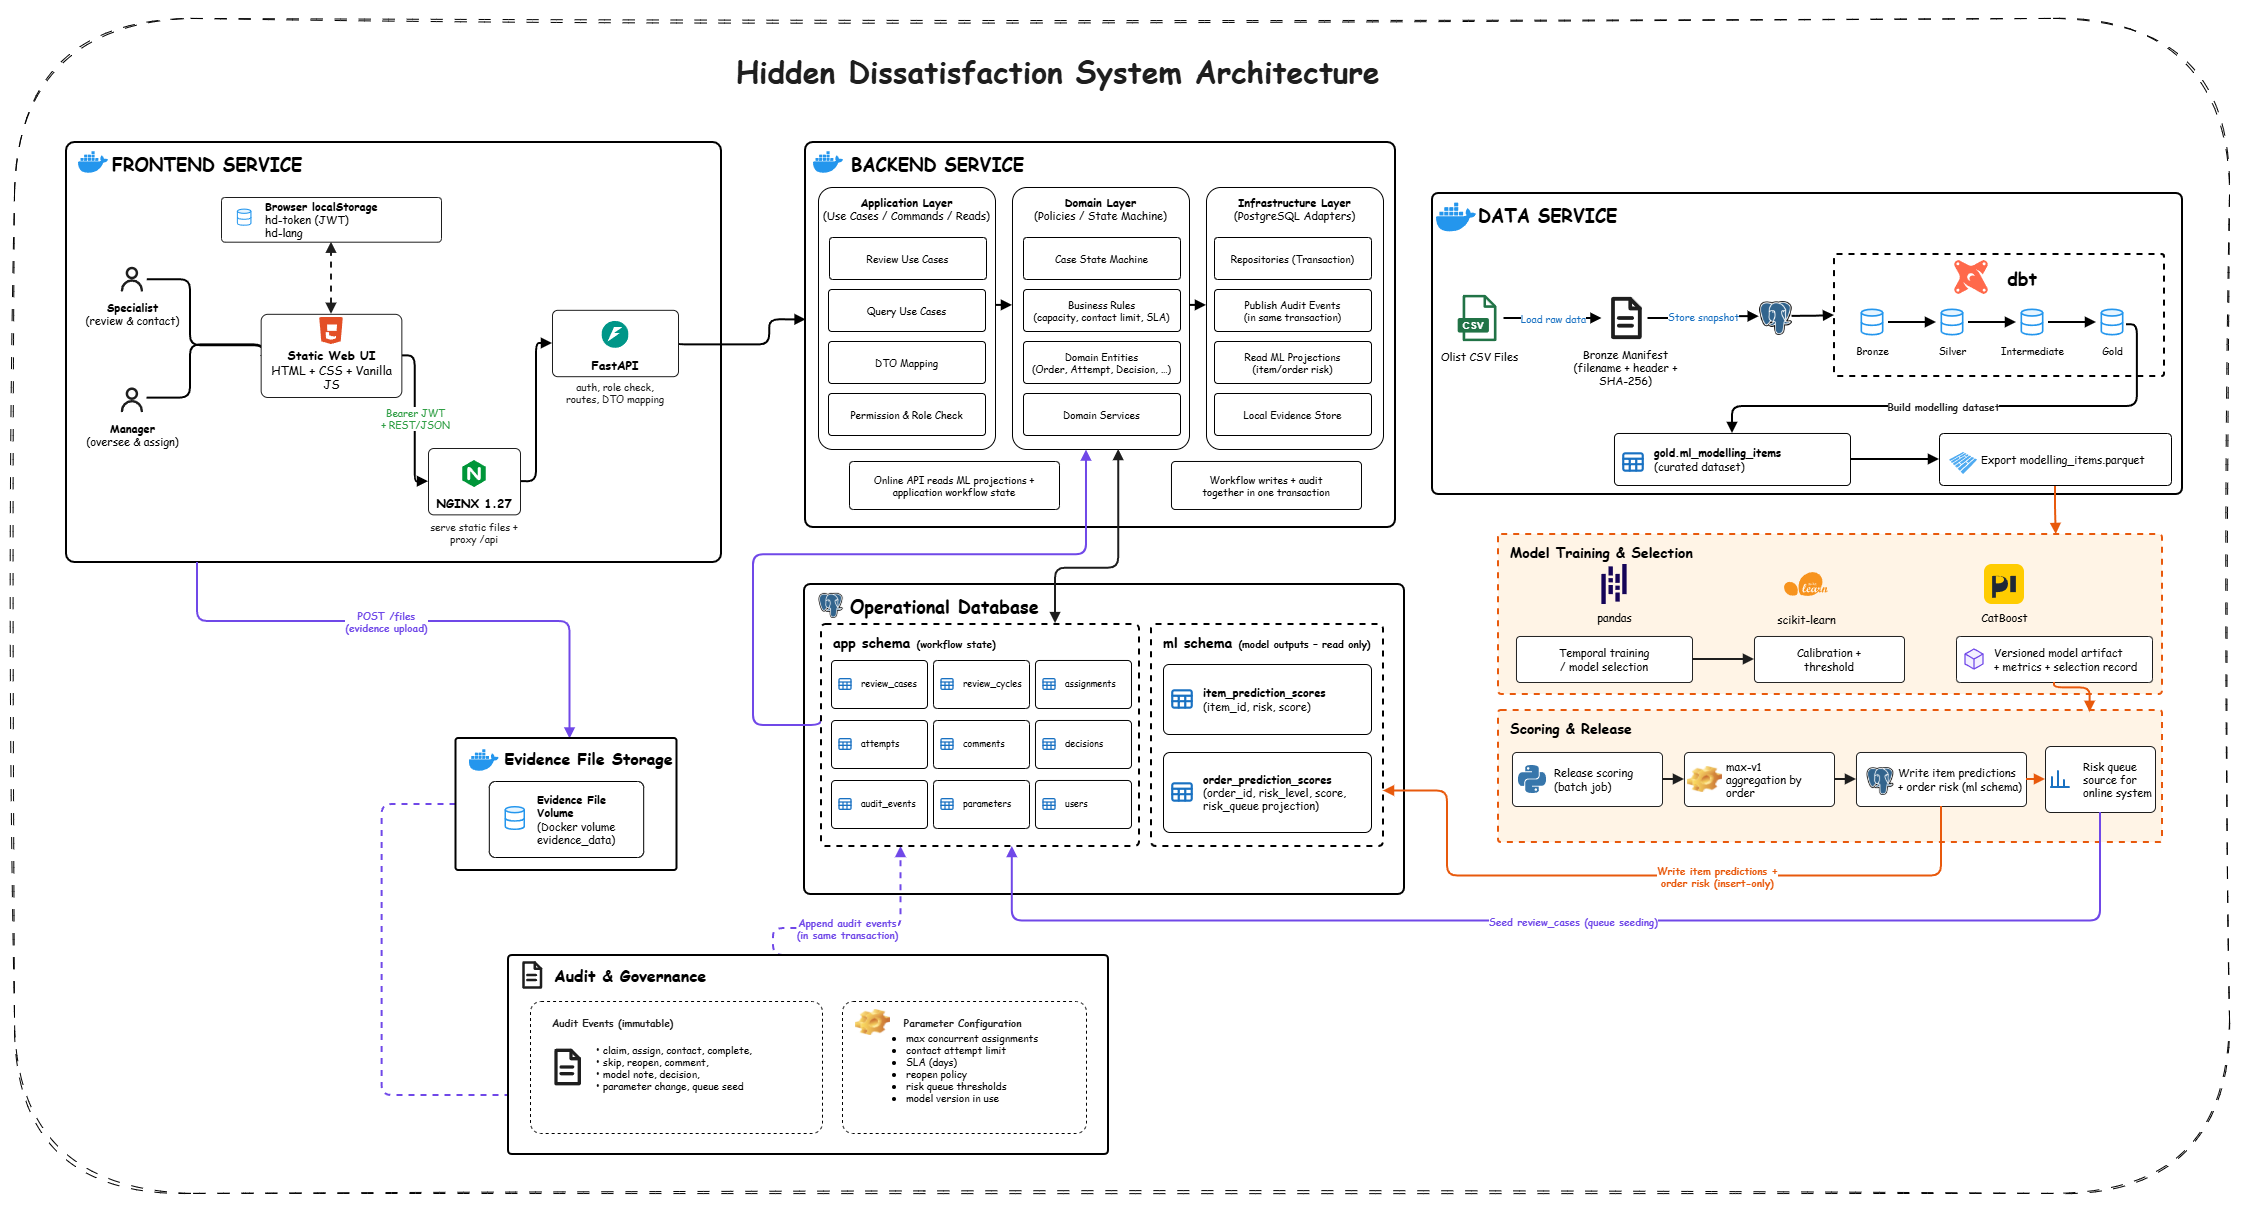
\includegraphics[width=\linewidth]{system-architecture}
  \caption{Kiến trúc tổng thể hệ thống}\label{fig:arch}
\end{figure}

\subsection{Đặc tả hệ thống}

Hệ thống được tổ chức theo kiến trúc phân lớp, với quy tắc phụ thuộc chỉ đi từ ngoài vào trong. Lớp \emph{miền nghiệp vụ} ở trung tâm chứa các quy tắc có ý nghĩa nghiên cứu: điều kiện vào quần thể, định nghĩa nhãn và các bất biến về thời gian. Lớp này không phụ thuộc thư viện dữ liệu hay mô hình nào, nên các quy tắc có thể được kiểm thử độc lập và không bị thay đổi ngầm khi đổi công cụ. Lớp \emph{ứng dụng} điều phối các ca sử dụng như nạp dữ liệu, huấn luyện và chấm điểm thông qua các giao diện trừu tượng. Lớp \emph{hạ tầng} hiện thực các giao diện đó bằng PostgreSQL và thư viện học máy cụ thể. Lớp \emph{giao diện} ngoài cùng cung cấp dòng lệnh cho tác vụ theo lô và API cho ứng dụng web. Nhờ cách tổ chức này, việc thay mô hình học máy chỉ chạm đến lớp hạ tầng.

Mô hình không được gọi theo thời gian thực mà chấm điểm theo lô. Một tác vụ chấm điểm toàn bộ item, tổng hợp điểm đơn theo max-v1, gán mức \textsc{Cao}, \textsc{Trung bình} hoặc \textsc{Thấp} theo ngưỡng đã chọn rồi ghi vào bảng dự đoán. Mỗi bản ghi lưu mã đơn, điểm rủi ro, mức ưu tiên và phiên bản mô hình, nên mọi điểm số đều truy vết được về đúng lần huấn luyện sinh ra nó. Lựa chọn này phù hợp với bản chất bài toán: thông tin đầu vào chỉ đầy đủ khi đơn đã giao, và nhân viên xử lý theo ca chứ không phản hồi từng giây, nên chấm điểm theo lô không làm mất giá trị dự báo mà giúp mọi người dùng nhìn thấy cùng một kết quả nhất quán.

Ứng dụng vận hành (backend FastAPI, giao diện web tĩnh qua NGINX, đóng gói bằng Docker Compose) chỉ đọc điểm rủi ro từ bảng dự đoán, không có thao tác nào ghi đè lên dự báo, và mọi thao tác ghi đều sinh sự kiện kiểm toán chỉ thêm. Nhờ đó dữ liệu vận hành sau này vẫn dùng được để đánh giá mô hình. Nhìn chung, kiến trúc hệ thống được thiết kế nhằm kết nối kết quả học máy với quy trình chăm sóc khách hàng mà vẫn giữ được sự độc lập giữa hai thành phần. Chi tiết về kiến trúc triển khai, vai trò người dùng, vòng đời xử lý trường hợp và các API được trình bày ở mục ~\ref{sec:system-api}.

% =====================================================================
\section{Dữ liệu và công cụ}\label{sec:data}

\subsection{Nguồn dữ liệu}

Nghiên cứu sử dụng bộ dữ liệu công khai \emph{Brazilian E-Commerce Public Dataset by Olist}~\cite{olist2018}, gồm khoảng 99\,000 đơn hàng phát sinh trên các sàn thương mại điện tử tại Brazil từ năm 2016 đến 2018. Bộ dữ liệu ghi nhận nhiều khía cạnh của quá trình mua sắm, từ thông tin khách hàng, sản phẩm và người bán đến thanh toán, vận chuyển và đánh giá sau mua.

Dữ liệu gồm chín bảng liên kết qua mã đơn, mã khách hàng, mã sản phẩm và mã người bán (Bảng~\ref{tab:olist}). Bảng đơn hàng là trung tâm, ghi các mốc của vòng đời đơn: mua, duyệt, bàn giao cho đơn vị vận chuyển, giao cho khách và ngày giao dự kiến. Những mốc thời gian này đặc biệt quan trọng đối với đề tài, bởi chúng được sử dụng để xác định đơn hàng có giao đúng hạn hay không và thiết lập thời điểm dự báo. Vì vậy, chất lượng của dữ liệu thời gian ảnh hưởng trực tiếp đến tính hợp lệ của quần thể nghiên cứu và khả năng kiểm soát rò rỉ thông tin.

\begin{table}[htbp]\centering\small
\caption{Các bảng trong bộ dữ liệu Olist}\label{tab:olist}
\begin{tabular}{llr}
\toprule
Bảng & Độ chi tiết (một dòng là) & Số dòng \\
\midrule
Đơn hàng                 & một đơn hàng                          &    99\,441 \\
Sản phẩm trong đơn       & một sản phẩm trong đơn                &   112\,650 \\
Thanh toán               & một lần thanh toán của đơn            &   103\,886 \\
Đánh giá                 & một đánh giá                          &    99\,224 \\
Khách hàng               & một khách hàng theo đơn               &    99\,441 \\
Người bán                & một người bán                         &     3\,095 \\
Sản phẩm                 & một sản phẩm                          &    32\,951 \\
Tọa độ địa lý            & một tọa độ theo mã bưu chính          & 1\,000\,163 \\
Dịch tên danh mục        & một danh mục (tiếng Bồ Đào Nha -- Anh) & 71 \\
\bottomrule
\end{tabular}
\end{table}

Mặc dù các bảng có thể liên kết với nhau, chúng không có cùng độ chi tiết. Đây là một vấn đề cần xử lý trước khi xây dựng tập dữ liệu mô hình hóa.

Cụ thể, bảng đánh giá gồm 99.224 dòng nhưng không phải mỗi đơn hàng đều có đúng một đánh giá. Một số đơn có nhiều đánh giá, trong khi những đơn khác không có đánh giá nào. Tương tự, bảng thanh toán có thể chứa nhiều dòng cho cùng một đơn hàng khi khách sử dụng nhiều phương thức thanh toán hoặc thanh toán theo nhiều kỳ.

Nếu nối trực tiếp các bảng này với bảng sản phẩm trong đơn, mỗi sản phẩm có thể bị nhân bản theo số lần thanh toán hoặc số đánh giá. Điều này làm thay đổi số lượng quan sát, ảnh hưởng đến tỷ lệ nhãn và khiến những đơn hàng có nhiều bản ghi liên quan đóng góp trọng số lớn hơn trong quá trình huấn luyện.

\subsection{Xây dựng tập dữ liệu mô hình hóa}

Từ chín bảng dữ liệu gốc, nhóm tiến hành xây dựng tập dữ liệu phục vụ mô hình học máy ở cấp sản phẩm trong đơn hàng. Để bảo đảm mỗi sản phẩm chỉ xuất hiện đúng một lần, các bảng thanh toán và đánh giá được tổng hợp về một dòng cho mỗi đơn trước khi thực hiện phép nối.

Đối với những đơn hàng có nhiều đánh giá, nhóm lựa chọn một đánh giá đại diện theo quy tắc ưu tiên đã xác định. Trước hết, những đánh giá đã được người bán phản hồi được ưu tiên lựa chọn. Nếu vẫn còn nhiều bản ghi, nhóm tiếp tục xét thời điểm phản hồi hoặc thời điểm tạo đánh giá mới nhất, sau đó sử dụng mã đánh giá làm tiêu chí phân định cuối cùng.

Mục đích của quy tắc này là bảo đảm tính tất định (deterministic) của quá trình xử lý. Nghĩa là khi sử dụng cùng một bộ dữ liệu đầu vào, hệ thống luôn lựa chọn cùng một đánh giá đại diện và tạo ra cùng một nhãn cho đơn hàng. Nhờ đó, kết quả thực nghiệm có thể được tái lập và kiểm tra khi cần thiết.

Sau khi xử lý độ chi tiết của các bảng, nhóm tiến hành xác định quần thể nghiên cứu. Một đơn hàng chỉ được đưa vào tập dữ liệu khi đáp ứng đồng thời ba điều kiện: (i) đã được giao thành công; (ii) ngày giao thực tế không muộn hơn ngày giao dự kiến; (iii) có đánh giá được tạo \emph{sau} thời điểm giao. Điều kiện (ii) định nghĩa phạm vi ``bất mãn ẩn'' của đề tài. Điều kiện (iii) ít hiển nhiên hơn nhưng không kém quan trọng: một đánh giá tạo trước hoặc đúng lúc giao là nhãn đã tồn tại tại thời điểm dự đoán, và giữ lại những đơn này sẽ đánh giá mô hình trên một tình huống không thể xảy ra trong vận hành. Bảng~\ref{tab:funnel} cho thấy số đơn và item còn lại sau mỗi bước lọc.

\begin{table}[htbp]\centering\small
\caption{Quá trình lọc quần thể nghiên cứu}\label{tab:funnel}
\begin{tabular}{lrr}
\toprule
Bước lọc & Đơn & Item \\
\midrule
Toàn bộ đơn hàng                          & 99\,441 & 112\,650 \\
Đã giao thành công                        & 96\,478 & 110\,197 \\
Giao đúng hoặc sớm hạn                    & 88\,644 & 101\,475 \\
Có đánh giá hợp lệ tạo sau thời điểm giao & 85\,420 &  97\,878 \\
\bottomrule
\end{tabular}
\end{table}

Kết quả cho thấy phần lớn đơn hàng đã giao trong dữ liệu Olist được hoàn thành đúng hoặc sớm hơn thời gian dự kiến. Bước lọc giao đúng hạn chỉ loại khoảng 8\% số đơn đã giao, nghĩa là quần thể ``giao đúng hạn'' chiếm phần lớn hoạt động của sàn chứ không phải một trường hợp biên. Trong quần thể này, tỉ lệ đơn nhận đánh giá thấp là 9,21\% (7\,865/85\,420): cứ khoảng mười một đơn giao đúng hạn lại có một đơn bị đánh giá 1--2 sao. Con số này đủ lớn để có ý nghĩa kinh doanh nhưng đủ nhỏ để tạo ra bài toán mất cân bằng lớp rõ rệt, định hướng trực tiếp các lựa chọn về xử lý mất cân bằng và chỉ số đánh giá ở các mục sau.

Bảng~\ref{tab:funnel} được dựng lại từ các tệp CSV gốc để kiểm toán. Snapshot dữ liệu đóng băng dùng cho huấn luyện có 85\,425 đơn và 97\,884 item, lệch 5 đơn và 6 item so với bản dựng lại. Nhật ký dbt xác nhận snapshot được tạo thành công và qua các kiểm tra về độ chi tiết và tính duy nhất, nhưng không lưu số đếm theo từng bước lọc nên chưa giải thích được chênh lệch. Với độ lệch dưới 0,01\%, ảnh hưởng đến các chỉ số là không đáng kể; các thí nghiệm sử dụng số liệu của snapshot đóng băng.

\subsection{Đặc trưng và kiểm soát rò rỉ dữ liệu}

Sau khi xác định quần thể nghiên cứu, bước tiếp theo là lựa chọn và xây dựng những đặc trưng có thể giúp mô hình nhận diện nguy cơ đánh giá thấp. Tuy nhiên, đây cũng là giai đoạn dễ phát sinh rò rỉ dữ liệu, đặc biệt khi thông tin về đơn hàng và đánh giá được lưu trữ trong những bảng có liên hệ trực tiếp với nhau.

Chẳng hạn, nếu nhóm tính điểm đánh giá trung bình của một người bán trên toàn bộ dữ liệu Olist, giá trị này có thể bao gồm cả đánh giá của đơn hàng đang được dự báo. Khi đó, mô hình đã gián tiếp sử dụng thông tin về kết quả cần dự đoán. Điều này có thể giúp chỉ số thực nghiệm tăng cao nhưng không phản ánh khả năng sử dụng trong thực tế, bởi tại thời điểm giao hàng, đánh giá của khách vẫn chưa xuất hiện.

Vì vậy, nhóm áp dụng nguyên tắc xuyên suốt: mọi đặc trưng phải biết được tại thời điểm $t_o$ (Hình~\ref{fig:leakage-timeline}).

Theo nguyên tắc này, các nhóm thông tin được phép gồm thông tin đơn và thanh toán; thuộc tính sản phẩm, danh mục và người bán; vị trí của khách và người bán; giá, phí vận chuyển và cấu trúc đơn; thời gian giao và khoảng dư so với ngày dự kiến; và các đặc trưng lịch sử tính hoàn toàn từ sự kiện xảy ra trước $t_o$. Các đầu vào bị cấm gồm điểm, nội dung, tiêu đề và thời điểm của đánh giá; mọi hành động xảy ra sau đánh giá; các thống kê tính trên toàn bộ dữ liệu; và các mã định danh, vốn không mang thông tin tổng quát nhưng cho phép mô hình học thuộc từng đối tượng. Danh sách đặc trưng được khai báo tường minh và pipeline tự động từ chối mọi cột bị cấm hoặc chưa khai báo, nên một sai sót khi thêm cột mới sẽ làm pipeline dừng thay vì âm thầm làm sai kết quả.

\begin{figure}[htbp]\centering
\begin{tikzpicture}[x=1cm,y=1cm,font=\small,
  ev/.style={circle,fill,inner sep=1.5pt},
  lab/.style={align=center,font=\footnotesize}]
  \fill[green!12] (0,0) rectangle (9,1.2);
  \fill[red!12]   (9,0) rectangle (13.5,1.2);
  \node[lab,green!45!black] at (4.5,1.45) {Được dùng làm đặc trưng};
  \node[lab,red!60!black]   at (11.25,1.45) {Bị cấm (rò rỉ)};
  \draw[-{Latex}] (0,0) -- (13.7,0) node[right]{$t$};
  \node[ev] at (3,0) {};   \node[lab,below] at (3,-0.1) {Mua hàng};
  \node[ev] at (5.5,0) {}; \node[lab,below] at (5.5,-0.1) {Seller\\gửi hàng};
  \draw[very thick] (9,-0.3) -- (9,1.2);
  \node[lab,below] at (9,-0.3) {\textbf{Giao hàng}\\$t_o$ (thời điểm dự đoán)};
  \node[ev] at (11.5,0) {}; \node[lab,below] at (11.5,-0.1) {Tạo đánh giá\\(nhãn $y$)};
  \draw[|-|,thick,blue!60!black] (0.2,0.6) -- (9,0.6) node[midway,above,lab]{Lịch sử của seller/danh mục từ các đơn trước $t_o$};
\end{tikzpicture}
\caption{Ranh giới thời gian của đặc trưng}
\label{fig:leakage-timeline}
\end{figure}

Các đặc trưng lịch sử của người bán và danh mục (số đánh giá trước đó, điểm đánh giá trung bình, thời gian xử lý và giao hàng trung bình) đòi hỏi ranh giới chặt hơn. Một đơn cũ chỉ được tính vào lịch sử khi cả thời điểm giao lẫn thời điểm đánh giá của nó đều diễn ra \emph{trước} $t_o$ của đơn đang xét. Điều kiện kép này cần thiết vì một đơn có thể đã giao trước $t_o$ nhưng được đánh giá sau $t_o$; nếu chỉ xét thời điểm giao, điểm đánh giá của đơn đó sẽ lọt vào đặc trưng dù tại thời điểm dự đoán chưa ai biết. Khi có ít hơn năm quan sát trước đó, trung bình lịch sử rất nhiễu, nên giá trị được để trống và một cờ ``hỗ trợ thấp'' được bật. Cờ này giúp mô hình phân biệt ``người bán mới, chưa có lịch sử'' với ``người bán có lịch sử tốt'', hai trường hợp có rủi ro rất khác nhau nhưng sẽ trông giống nhau nếu điền giá trị thiếu bằng trung bình chung.

Tập đặc trưng cuối cùng gồm 61 đặc trưng chia thành bảy nhóm (Bảng~\ref{tab:features}; danh sách đầy đủ ở Phụ lục~\ref{app:features}). Các nhóm được xây dựng theo giả thuyết về nguồn gốc của bất mãn khi giao hàng không phải là vấn đề. Nhóm \emph{tốc độ và độ biến động của người bán} xuất phát từ quan sát rằng hiệu quả giao hàng ảnh hưởng đến điểm đánh giá~\cite{ravula2023,deshpande2023}: một người bán thường xuyên giao chậm hoặc thất thường có thể vẫn kịp hạn ở đơn đang xét nhưng phản ánh chất lượng vận hành chung thấp. Nhóm \emph{cấu trúc đơn} (số lượng, tỉ lệ và mức độ tập trung theo người bán và danh mục) được gợi ý từ bằng chứng rằng giao hàng tách thành nhiều kiện làm giảm sự hài lòng~\cite{brylla2022}. Do Olist không ghi thời điểm giao riêng cho từng item, số người bán và số sản phẩm trong đơn chỉ là đại diện gián tiếp cho việc tách kiện. Các nhóm \emph{hình thái sản phẩm} và \emph{độ đầy đủ nội dung} nhắm đến khoảng cách giữa kỳ vọng và thực tế: sản phẩm cồng kềnh dễ hư hỏng khi vận chuyển, còn trang sản phẩm thiếu ảnh hoặc mô tả dễ khiến khách nhận được thứ khác với hình dung.

\begin{table}[htbp]\centering\small
\caption{Các nhóm đặc trưng trong tập cuối cùng}\label{tab:features}
\begin{tabular}{p{4.2cm}p{9cm}}
\toprule
Nhóm & Nội dung chính \\
\midrule
Cơ sở (24) & Giá, phí vận chuyển, thanh toán, thời gian giao, khoảng dư so với ngày dự kiến, kích thước sản phẩm, lịch sử đánh giá của seller và danh mục kèm cờ hỗ trợ thấp, danh mục, bang của khách \\
Tốc độ và độ biến động của seller (7) & Thời gian trung bình từ duyệt đơn đến bàn giao vận chuyển và đến khi giao, độ lệch chuẩn, hệ số biến thiên, tỉ lệ phí vận chuyển \\
Số lượng trong đơn (7) & Số seller, danh mục, sản phẩm; cờ nhiều item, nhiều seller, nhiều danh mục \\
Tỉ lệ trong đơn (4) & Tổng phí vận chuyển, tỉ trọng phí vận chuyển, tỉ trọng giá trị lớn nhất và nhỏ nhất của item \\
Mức độ tập trung (2) & Chỉ số Herfindahl--Hirschman theo danh mục và theo seller \\
Hình thái sản phẩm (13) & Thể tích, mật độ, tỉ lệ kích thước, phí vận chuyển trên giá và trên khối lượng, các cờ thiếu hoặc bằng không \\
Độ đầy đủ nội dung (4) & Độ dài tên và mô tả, số trường mô tả bị thiếu \\
\bottomrule
\end{tabular}
\end{table}

\subsection{Công cụ}

Để triển khai quy trình xử lý dữ liệu và học máy, nhóm sử dụng Python làm ngôn ngữ lập trình chính, kết hợp với các thư viện chuyên dụng cho từng giai đoạn.

Trong quá trình xử lý dữ liệu, pandas, NumPy và PyArrow được sử dụng để đọc, biến đổi và quản lý các tập dữ liệu. Đối với bước xây dựng mô hình, nhóm sử dụng scikit-learn và CatBoost để huấn luyện, đánh giá và hiệu chỉnh xác suất. Các mô hình sau khi huấn luyện được lưu trữ bằng joblib để phục vụ việc tái sử dụng và triển khai. Bên cạnh các thư viện Python, hệ thống sử dụng PostgreSQL làm kho lưu trữ dữ liệu và dbt để tổ chức những phép biến đổi trong kho dữ liệu. Phiên bản cụ thể của từng công cụ được trình bày tại Phụ lục ~\ref{app:env}. 

Một yêu cầu quan trọng trong quá trình triển khai là khả năng tái lập kết quả (reproducibility). Để bảo đảm các thí nghiệm có thể được thực hiện lại trong cùng điều kiện, nhóm tập trung quản lý những thông số quan trọng trong các tệp cấu hình có kiểm soát phiên bản, thay vì khai báo rải rác trong nhiều notebook.

Các thông tin được quản lý bao gồm ranh giới thời gian, danh sách biến thể mô hình, siêu tham số và những lựa chọn xử lý dữ liệu. Mỗi lần chạy sử dụng seed cố định và giới hạn số luồng tính toán nhằm giảm sự khác biệt giữa các lần thực nghiệm. Sau khi hoàn tất, hệ thống tạo báo cáo ghi lại cấu hình đã sử dụng, số lượng quan sát trong từng phân vùng, các chỉ số đánh giá và mã commit của phiên bản mã nguồn. Nhờ đó, những kết quả được trình bày ở Chương 4 có thể được đối chiếu với đúng cấu hình và phiên bản chương trình đã tạo ra chúng.

Về tổ chức dữ liệu, kho dữ liệu được tổ chức theo kiến trúc medallion, trong đó mỗi tầng có một mức cam kết chất lượng khác nhau. Tầng \emph{bronze} lưu dữ liệu nguyên dạng kèm manifest chống nạp trùng, đóng vai trò bản gốc để mọi tầng sau có thể dựng lại. Tầng \emph{silver} chuẩn hóa kiểu dữ liệu và gộp tọa độ theo mã bưu chính. Tầng \emph{intermediate} chứa logic nghiệp vụ: quần thể nghiên cứu, đánh giá đại diện, đặc trưng lịch sử và các nhóm đặc trưng trong Bảng~\ref{tab:features}. Tầng \emph{gold} gồm các bảng sự kiện và chiều phục vụ dashboard cùng bảng mô hình hóa mức item phục vụ huấn luyện. Sau mỗi lần build, dbt tự động kiểm tra tính duy nhất của khóa và độ chi tiết của bảng, còn các đặc trưng lịch sử có kiểm thử riêng bảo đảm không sử dụng sự kiện từ tương lai. 

Việc đặt những quy tắc kiểm soát rò rỉ ngay trong kho dữ liệu, thay vì chỉ thực hiện trong mã huấn luyện, là một lựa chọn có chủ đích. Cách tổ chức này giúp các đặc trưng được tính toán nhất quán tại một nơi, đồng thời bảo đảm những mô hình khác nhau sử dụng chung một định nghĩa dữ liệu. Nhờ vậy, khi thay đổi thuật toán, nhóm vẫn có thể so sánh kết quả trên cùng một cơ sở dữ liệu và quy tắc xử lý.

% =====================================================================
\section{Mô hình và thuật toán}\label{sec:models}

Sau khi hoàn tất quá trình xây dựng dữ liệu và đặc trưng, nhóm tiến hành lựa chọn phương pháp học máy phù hợp với bài toán dự báo bất mãn ẩn. Do dữ liệu Olist chủ yếu được tổ chức dưới dạng bảng, bao gồm cả biến số và biến phân loại, nhóm ưu tiên những thuật toán có khả năng khai thác các mối quan hệ trong dữ liệu có cấu trúc.

Tuy nhiên, mục tiêu của quá trình thực nghiệm không chỉ là tìm ra mô hình có chỉ số dự báo cao nhất. Nhóm còn cần xác định liệu việc sử dụng một thuật toán phức tạp hơn có thực sự mang lại lợi ích so với những phương pháp đơn giản, cũng như đánh giá mức độ ổn định của kết quả qua các giai đoạn thời gian.

Vì vậy, quá trình xây dựng mô hình được tổ chức theo hướng so sánh các ứng viên, kiểm soát tiền xử lý, xử lý mất cân bằng lớp, lựa chọn mô hình theo thời gian và hiệu chỉnh xác suất trước khi đưa kết quả vào danh sách ưu tiên.

\subsection{Mô hình cơ sở và ứng viên}

Để đánh giá giá trị bổ sung của học máy, nhóm xây dựng tập mô hình ứng viên theo mức độ phức tạp tăng dần. Cách tiếp cận này giúp xác định liệu những thuật toán có khả năng học các mối quan hệ phức tạp có thực sự cải thiện kết quả so với các phương pháp đơn giản hơn hay không.

Nhóm so sánh các mô hình theo độ phức tạp tăng dần, để mỗi mức phức tạp thêm vào đều phải chứng minh được giá trị so với mức trước. Mức sàn là \emph{mô hình theo tỉ lệ nền}, dự đoán mọi item bằng tỉ lệ dương của tập huấn luyện; một ứng viên không vượt qua mức này không học được gì từ đặc trưng. Tiếp theo là \emph{hồi quy logistic} với hai mức điều chuẩn $C \in \{0{,}1;\,1\}$, đại diện cho quan hệ tuyến tính và dễ diễn giải. Ba họ mô hình cây có khả năng nắm bắt tương tác phi tuyến được đưa vào sau đó: \emph{rừng ngẫu nhiên} với hai cấu hình (độ sâu 8, tối thiểu 5 mẫu mỗi lá và độ sâu 12, tối thiểu 10 mẫu mỗi lá), \emph{HistGradientBoosting} với hai cấu hình (L2 $=1$, 31 lá và L2 $=5$, 15 lá), và \emph{CatBoost} với độ sâu 6, 8 và 10, vốn có cơ chế riêng để xử lý biến phân loại nhiều giá trị như danh mục sản phẩm. Các nghiên cứu trước trên Olist cho thấy mô hình cây thường cạnh tranh tốt với học sâu trên dữ liệu bảng~\cite{zaghloul2024}, nên nhóm không đưa mạng nơ-ron vào so sánh. Cần lưu ý rằng đây là không gian ứng viên đã khai báo; kho kết quả hiện lưu đủ số liệu theo fold cho rừng ngẫu nhiên và các cấu hình CatBoost, còn các họ khác chưa có bảng chỉ số đồng nhất (Chương~4).

Song song với mô hình, nhóm thử bốn chế độ huấn luyện nhằm xử lý sự lệch pha giữa item và đơn đã nêu ở mục~\ref{sec:pipeline}. Chế độ \emph{item-unweighted} cho mọi item trọng số như nhau, khiến các đơn nhiều sản phẩm chi phối quá trình học. Chế độ \emph{order-weight} đặt trọng số mỗi item bằng nghịch đảo số item trong đơn để mỗi đơn đóng góp như nhau. Chế độ \emph{order-reference} và \emph{order-aggregate} gộp item thành một dòng mỗi đơn trước khi huấn luyện, khớp trực tiếp với mức của nhãn và của chỉ số chính, nhưng đánh đổi bằng việc mất thông tin chi tiết ở mức sản phẩm. 

Việc so sánh bốn chế độ nhằm xác định liệu học ở cấp sản phẩm có thực sự mang lại lợi ích so với việc xây dựng mô hình trực tiếp ở cấp đơn hàng. Đây cũng là cơ sở để đánh giá ảnh hưởng của nhãn yếu và cấu trúc nhiều sản phẩm trong một đơn đối với kết quả dự báo.

\subsection{Tiền xử lý}

Các mô hình học máy được lựa chọn có những yêu cầu khác nhau đối với dữ liệu đầu vào. Vì vậy, nhóm không áp dụng một quy trình tiền xử lý duy nhất cho tất cả thuật toán, mà xây dựng những nhánh xử lý phù hợp với đặc điểm của từng họ mô hình.

Đối với hồi quy logistic và Random Forest, các biến số được xử lý giá trị thiếu bằng trung vị của tập huấn luyện. Riêng hồi quy logistic được bổ sung bước chuẩn hóa, bởi thuật toán này nhạy với sự khác biệt về thang đo giữa các đặc trưng. Chẳng hạn, giá trị đơn hàng và số lượng sản phẩm có thể nằm trên những khoảng giá trị rất khác nhau, khiến quá trình tối ưu bị ảnh hưởng nếu không được chuẩn hóa.

Với các biến phân loại, nhóm điền giá trị thiếu bằng giá trị xuất hiện phổ biến nhất, sau đó sử dụng phương pháp mã hóa one-hot để chuyển chúng thành các biến mà mô hình có thể xử lý. Những giá trị phân loại chưa từng xuất hiện trong tập huấn luyện được bỏ qua khi gặp ở dữ liệu mới, thay vì khiến pipeline phát sinh lỗi.

Đối với HistGradientBoosting, nhóm sử dụng phương pháp mã hóa thứ tự cho các biến phân loại. Cách xử lý này giúp duy trì cấu trúc ma trận dữ liệu phù hợp với cơ chế chia nhánh theo biểu đồ tần suất của thuật toán.

Trong khi đó, CatBoost có khả năng tiếp nhận trực tiếp các biến phân loại, nên không cần thực hiện mã hóa one-hot như những mô hình còn lại.

Mặc dù các bước xử lý khác nhau, tất cả nhánh tiền xử lý đều tuân theo cùng một nguyên tắc: mọi phép biến đổi cần học tham số từ dữ liệu chỉ được fit trên tập huấn luyện của từng fold.

Chẳng hạn như trung vị dùng để điền giá trị thiếu phải được tính từ tập huấn luyện, không phải từ toàn bộ dữ liệu. Tương tự, danh sách các giá trị phân loại phục vụ mã hóa cũng chỉ được xác định từ những quan sát mà mô hình được phép sử dụng tại thời điểm huấn luyện.

Nếu những thống kê này được tính trên toàn bộ dữ liệu trước khi chia tập, thông tin từ giai đoạn kiểm định có thể ảnh hưởng đến quá trình xử lý đầu vào. Mặc dù không trực tiếp sử dụng nhãn, đây vẫn là một dạng rò rỉ dữ liệu có thể khiến kết quả đánh giá thiếu khách quan.

Để hạn chế rủi ro trên, nhóm đặt các bước tiền xử lý trong cùng một pipeline với mô hình. Nhờ đó, khi thực hiện kiểm định rolling-origin, mỗi fold sẽ tự xây dựng các tham số tiền xử lý từ dữ liệu huấn luyện tương ứng và áp dụng chúng lên dữ liệu kiểm định mà không sử dụng thông tin tương lai.

\subsection{Xử lý mất cân bằng lớp}

Một đặc điểm quan trọng của tập dữ liệu nghiên cứu là số quan sát thuộc nhóm đánh giá thấp chiếm tỷ lệ nhỏ hơn đáng kể so với nhóm còn lại. Tùy theo giai đoạn thời gian, tỷ lệ nhãn dương ở cấp sản phẩm dao động khoảng 9--14\%. Có hai hướng tiếp cận phổ biến: thay đổi dữ liệu bằng cách lấy mẫu lại (như SMOTE), hoặc thay đổi hàm mất mát bằng trọng số lớp. 

Trong đề tài, nhóm lựa chọn trọng số lớp kết hợp với việc xác định ngưỡng ưu tiên riêng, thay vì sử dụng SMOTE trong pipeline chính. Chẳng hạn, đối với Random Forest, nhóm sử dụng cơ chế trọng số cân bằng được tính lại trên từng mẫu bootstrap. Lựa chọn này dựa trên hai bằng chứng. Thứ nhất, với các bộ phân loại mạnh như mô hình boosting, cân bằng dữ liệu bằng SMOTE hầu như không cải thiện so với việc chỉ tối ưu ngưỡng quyết định~\cite{elor2022smote}. Thứ hai, mọi phương pháp hiệu chỉnh mất cân bằng đều làm xác suất dự đoán bị đẩy lên một cách có hệ thống~\cite{vandengoorbergh2022}. Hệ quả thứ hai đặc biệt quan trọng với bài toán này, vì hàng đợi ưu tiên và mức rủi ro đều dựa vào xác suất. Trọng số lớp vì vậy được xem như một công cụ giúp mô hình học lớp thiểu số, còn độ lệch xác suất mà nó gây ra được sửa ở bước hiệu chỉnh. 

Trong phạm vi hiện tại, SMOTE chỉ được xem là một hướng thử nghiệm bổ sung và chưa được đưa vào quy trình chính. Cách lựa chọn này giúp giữ nguyên phân bố dữ liệu quan sát trong quá trình xây dựng tập huấn luyện, đồng thời tập trung vào khả năng xếp hạng và độ tin cậy của xác suất.

\subsection{Chia dữ liệu theo thời gian và lựa chọn mô hình}

Sau khi xác định các mô hình ứng viên và phương pháp tiền xử lý, nhóm cần xây dựng một quy trình đánh giá có khả năng phản ánh điều kiện sử dụng thực tế. Đây là bước đặc biệt quan trọng, bởi cách chia dữ liệu có thể ảnh hưởng đáng kể đến kết quả so sánh giữa các thuật toán.

Các nghiên cứu trước trên Olist thường chia ngẫu nhiên 80:20~\cite{orman2026}. Cách chia này cho phép mô hình học từ các đơn diễn ra \emph{sau} đơn đang kiểm định, chẳng hạn biết một người bán bắt đầu bị đánh giá kém từ tháng sau, nên thường cho kết quả lạc quan hơn triển khai thực tế. Nhóm vì vậy sắp dữ liệu theo thời điểm dự đoán $t_o$ và chia thành sáu phân vùng liên tiếp (Bảng~\ref{tab:split}). Mỗi phân vùng là khoảng nửa mở $[\text{đầu}, \text{cuối})$, mọi item của một đơn nằm cùng phân vùng, và mỗi phân vùng chỉ phục vụ đúng một mục đích. Nguyên tắc ``một phân vùng, một quyết định'' bảo đảm không quyết định nào được đánh giá trên dữ liệu đã dùng để đưa ra một quyết định trước đó, nhờ vậy sai lệch lạc quan không tích lũy qua các bước.

\begin{table}[htbp]\centering\small
\caption{Phân vùng dữ liệu theo thời gian dự đoán}\label{tab:split}
\begin{tabular}{lllrrr}
\toprule
Phân vùng & Từ & Đến (không gồm) & Đơn & Item & Tỉ lệ dương (item) \\
\midrule
Huấn luyện            & 2016-10-11 & 2017-10-01 & 23\,545 & 26\,708 & 10,13\% \\
Lựa chọn mô hình      & 2017-10-01 & 2017-12-01 &  8\,586 &  9\,957 & 11,92\% \\
Fit hiệu chỉnh        & 2017-12-01 & 2018-02-01 & 11\,759 & 13\,444 & 12,74\% \\
So sánh hiệu chỉnh    & 2018-02-01 & 2018-04-01 & 10\,623 & 12\,265 & 13,80\% \\
Chọn ngưỡng           & 2018-04-01 & 2018-06-01 & 12\,351 & 14\,319 & 11,61\% \\
Test niêm phong       & 2018-06-01 & 2018-09-01 & 18\,561 & 21\,191 & ẩn \\
\bottomrule
\end{tabular}
\end{table}

Bảng~\ref{tab:split} cũng cho thấy tỉ lệ dương không đứng yên mà dao động từ 10,13\% đến 13,80\% giữa các phân vùng. Các tỉ lệ này tính ở mức item nên cao hơn tỉ lệ 9,21\% ở mức đơn của Bảng~\ref{tab:funnel}, vì đơn nhiều sản phẩm có tỉ lệ đánh giá thấp cao hơn và đóng góp nhiều dòng hơn; ở mức đơn, năm phân vùng phát triển có tỉ lệ dương 8,86--10,53\% (mục~\ref{subsec:eda-labels}). Sự dịch chuyển này là lý do trực tiếp khiến hiệu chỉnh xác suất và chọn ngưỡng phải được thực hiện trên dữ liệu gần thời điểm triển khai hơn dữ liệu huấn luyện: một mô hình được hiệu chỉnh theo tỉ lệ 10\% của năm 2017 sẽ đánh giá thấp rủi ro khi tỉ lệ thực tế đã tăng lên. Phân vùng test cuối cùng được thiết kế để niêm phong: tỉ lệ dương của nó không được báo cáo và không được dùng cho bất kỳ bước hiệu chỉnh hay chọn ngưỡng nào. Tuy nhiên, giai đoạn thời gian này đã được biết đến trong quá trình phát triển, nên nó không còn là holdout xác nhận hoàn toàn độc lập (xem mục~\ref{subsec:res-scope}).

Bên trong giai đoạn huấn luyện, các biến thể được so sánh bằng kiểm định rolling-origin với cửa sổ mở rộng gồm ba fold (Hình~\ref{fig:temporal-folds}). Ở mỗi fold, mô hình học trên toàn bộ dữ liệu trước mốc cắt và được đánh giá trên đoạn ngay sau đó, mô phỏng đúng cách mô hình được huấn luyện lại định kỳ trong thực tế. Ba fold thay vì một cho phép quan sát độ ổn định của từng biến thể qua thời gian, tránh chọn nhầm một biến thể chỉ tốt nhờ may mắn ở một giai đoạn. Biến thể được chọn theo thứ tự ưu tiên: PR-AUC mức đơn (theo max-v1) trung bình qua các fold cao nhất; nếu ngang nhau thì chọn biến thể có Brier score thấp hơn; nếu vẫn ngang nhau thì chọn mô hình đơn giản hơn. Hiệu chỉnh xác suất và chọn ngưỡng không tham gia vào bước này để tách biệt câu hỏi ``mô hình nào xếp hạng tốt nhất'' khỏi câu hỏi ``xác suất có đáng tin không''.

\begin{figure}[htbp]\centering
\begin{tikzpicture}[x=0.62cm,y=1cm,font=\footnotesize]
  % trục: tháng 0 = 2016-10; 23 = 2018-09
  \def\seg#1#2#3#4{\fill[#3] (#1,0) rectangle (#2,0.6); \node[font=\scriptsize] at ({(#1+#2)/2},0.3) {#4};}
  \seg{0}{12}{blue!30}{Huấn luyện}
  \seg{12}{14}{orange!55}{A}
  \seg{14}{16}{teal!40}{B}
  \seg{16}{18}{teal!25}{C}
  \seg{18}{20}{violet!30}{D}
  \seg{20}{23}{red!50}{Test}
  % 3 fold rolling-origin trong train; mốc thật, đơn vị tháng từ 2016-10-01:
  % 2017-06-01=8.0, 2017-07-18=9.57, 2017-08-24=10.77, 2017-10-01=12.0
  \foreach \k/\s/\e in {1/8.0/9.57,2/9.57/10.77,3/10.77/12.0} {
    \fill[blue!30] (0,-0.4*\k) rectangle (\s,-0.4*\k+0.28);
    \fill[orange!55] (\s,-0.4*\k) rectangle (\e,-0.4*\k+0.28);
    \node[left] at (0,-0.4*\k+0.14) {Fold \k};
  }
  \draw[densely dotted] (8,-1.3) -- (8,-1.55) node[below,font=\scriptsize]{2017-06};
  \draw[-{Latex}] (0,-1.55) -- (23.6,-1.55);
  \foreach \m/\l in {0/2016-10,12/2017-10,14/2017-12,16/2018-02,18/2018-04,20/2018-06,23/2018-09}
    \draw (\m,-1.5) -- (\m,-1.6) node[below,rotate=40,anchor=north east,font=\scriptsize]{\l};
  \node[align=left,anchor=north west,font=\scriptsize] at (0,-2.7)
    {A: lựa chọn mô hình \quad B: fit hiệu chỉnh \quad C: so sánh hiệu chỉnh \quad D: chọn ngưỡng \quad Test: test niêm phong};
\end{tikzpicture}
\caption{Thiết kế chia dữ liệu theo thời gian}
\label{fig:temporal-folds}
\end{figure}

\subsection{Hiệu chỉnh xác suất và ngưỡng ưu tiên}

Sau khi lựa chọn mô hình, nhóm tiếp tục xem xét độ tin cậy của xác suất dự báo. Đây là bước cần thiết bởi một mô hình có thể sắp xếp đúng thứ tự rủi ro nhưng vẫn ước lượng sai mức xác suất thực tế.

Một mô hình có thể xếp hạng tốt nhưng xác suất sai: nếu mô hình nói ``rủi ro 40\%'' cho một nhóm đơn mà thực tế chỉ 15\% bị đánh giá thấp, quản lý sẽ ước lượng sai khối lượng công việc và mức độ nghiêm trọng. Trọng số lớp và sự dịch chuyển tỉ lệ dương theo thời gian đều gây ra loại sai lệch này, nên nhóm hiệu chỉnh xác suất sau khi đã chọn mô hình. Mô hình gốc được huấn luyện lại trên phân vùng huấn luyện và lựa chọn. Hai phương pháp hiệu chỉnh được fit trên phân vùng \emph{fit hiệu chỉnh}: sigmoid (Platt scaling), giả định độ lệch có dạng hàm logistic và ổn định khi dữ liệu ít, và isotonic, không giả định dạng hàm nhưng dễ quá khớp. Hai phương pháp sau đó được so sánh bằng Brier score trên phân vùng \emph{so sánh hiệu chỉnh} độc lập; nếu không phương pháp nào cải thiện so với mô hình gốc, mô hình gốc được giữ nguyên. Việc tách hai phân vùng giúp kết quả so sánh không bị lạc quan do đánh giá trên chính dữ liệu đã dùng để fit, một sai lầm đặc biệt dễ xảy ra với isotonic. Với mô hình rừng ngẫu nhiên được giữ lại, Brier score trên phân vùng so sánh là 0,220 khi chưa hiệu chỉnh, 0,106 với isotonic và 0,105 với sigmoid, nên sigmoid được chọn. Hiệu chỉnh là phép biến đổi đơn điệu nên không làm thay đổi thứ tự xếp hạng, do đó PR-AUC và Recall@5\% không bị ảnh hưởng, chỉ độ tin cậy của xác suất được cải thiện.

Ngưỡng ưu tiên được chọn trên phân vùng \emph{chọn ngưỡng}: các đơn thuộc 5\% điểm rủi ro cao nhất được gán mức \textsc{Cao}, các đơn còn lại trong 20\% cao nhất được gán mức \textsc{Trung bình}. Nhóm chọn ngưỡng theo tỉ lệ phần trăm thay vì một ngưỡng xác suất cố định như 0,5 vì ràng buộc thực sự của bộ phận chăm sóc khách hàng là số đơn có thể xử lý mỗi ngày, không phải mức xác suất. Ngưỡng phần trăm biến năng lực xử lý thành tham số trực tiếp của mô hình, và vẫn giữ nguyên ý nghĩa khi tỉ lệ dương dịch chuyển, điều mà một ngưỡng xác suất cố định không làm được. Cách tiếp cận này phù hợp với quan điểm rằng giá trị của mô hình nằm ở việc phân bổ nguồn lực can thiệp có hạn~\cite{gomezvargas2025}.

Nhìn chung, bước hiệu chỉnh xác suất và xác định ngưỡng giúp chuyển kết quả học máy từ những điểm dự báo riêng lẻ thành thông tin có thể sử dụng trong quy trình chăm sóc khách hàng. Tuy nhiên, các mức ưu tiên chỉ thể hiện thứ tự rủi ro tương đối, không đồng nghĩa với việc hệ thống đã chứng minh được hiệu quả của một hành động can thiệp cụ thể.

% =====================================================================
\section{Phương pháp đánh giá}\label{sec:eval}

Để đánh giá mô hình một cách phù hợp với mục tiêu nghiên cứu, nhóm không chỉ xem xét khả năng dự đoán đúng trên toàn bộ dữ liệu mà tập trung vào những chỉ số phản ánh việc nhận diện các đơn hàng có nguy cơ nhận đánh giá thấp.

Nguyên nhân là tỷ lệ nhãn dương trong quần thể nghiên cứu chỉ chiếm khoảng một phần mười. Trong điều kiện này, một mô hình luôn dự đoán mọi đơn hàng thuộc nhóm không bị đánh giá thấp vẫn có thể đạt accuracy gần 90\%. Nhóm dùng ba chỉ số, mỗi chỉ số trả lời một câu hỏi khác nhau về mô hình, tính trên đoạn kiểm định của từng fold rồi lấy trung bình qua ba fold.

\textbf{PR-AUC} (diện tích dưới đường cong precision--recall) trả lời câu hỏi \emph{mô hình xếp hạng tốt đến đâu} và là chỉ số chính. Khác với ROC-AUC, PR-AUC tập trung vào lớp dương và không bị thổi phồng bởi số lượng lớn các đơn âm dễ phân loại, nên phù hợp với bài toán mất cân bằng. Chỉ số được đo ở cả mức item và mức đơn (sau khi tổng hợp bằng max-v1); mức đơn là mức quyết định vì đó là đơn vị nhân viên xử lý. PR-AUC của một mô hình xếp hạng ngẫu nhiên xấp xỉ tỉ lệ dương, nên tỉ lệ dương của từng fold là mốc so sánh tự nhiên.

\textbf{Brier score} trả lời câu hỏi \emph{xác suất có đáng tin không}:
\begin{equation}\label{eq:brier}
  \mathrm{BS} = \frac{1}{N}\sum_{j=1}^{N}\left(\hat{p}_j - y_j\right)^2
\end{equation}
trong đó $\hat p_j$ là xác suất dự đoán ở mức đơn và $y_j \in \{0,1\}$ là nhãn thực tế; giá trị càng thấp càng tốt. Brier score phạt cả xếp hạng kém lẫn xác suất lệch, nên hai mô hình có cùng PR-AUC vẫn có thể có Brier score khác nhau. Đây cũng là tiêu chí so sánh các phương pháp hiệu chỉnh ở mục~\ref{sec:models}.

\textbf{Recall@5\%} trả lời câu hỏi vận hành: \emph{nếu chỉ xử lý được 5\% số đơn, nhóm này bắt được bao nhiêu phần đơn bị đánh giá thấp?} Mức 5\% tương ứng với nhóm ưu tiên \textsc{Cao}. Chọn ngẫu nhiên 5\% số đơn chỉ cho recall kỳ vọng 5\%, nên tỉ số giữa Recall@5\% của mô hình và 5\% cho biết mô hình giúp bộ phận chăm sóc khách hàng hiệu quả gấp bao nhiêu lần so với không có mô hình. Mức tham chiếu ngẫu nhiên là mốc tối thiểu; các nghiên cứu về ưu tiên hóa cho thấy những luật xếp hạng đơn giản như sắp theo giá trị đơn đôi khi đã khó vượt qua~\cite{li2026valuesorting}, nên đây là hướng so sánh cần bổ sung.

Ba chỉ số này đo khả năng \emph{dự báo} chứ không đo hiệu quả \emph{can thiệp}. Một đơn rủi ro cao không nhất thiết là đơn mà việc liên hệ sẽ thay đổi được kết quả; nghiên cứu về giữ chân khách hàng đã chỉ ra rằng nhắm vào khách có rủi ro cao nhất không phải lúc nào cũng mang lại hiệu quả cao nhất~\cite{ascarza2018}. Đánh giá hiệu quả can thiệp đòi hỏi thử nghiệm có đối chứng và nằm ngoài phạm vi đề tài. Ngoài ra, các kết quả trình bày ở Chương~4 là kết quả trên các fold phát triển. Phân vùng test chưa được dùng để chấm điểm; vì giai đoạn này đã được biết trong quá trình phát triển, một đánh giá xác nhận hợp lệ cần một holdout thay thế mới. Các con số ở Chương~4 vì vậy mang tính thăm dò, chưa phải ước lượng cuối cùng về hiệu năng khi triển khai.

Thông qua phương pháp thực hiện trên, nhóm xây dựng được một quy trình kết nối dữ liệu, mô hình học máy và hệ thống hỗ trợ chăm sóc khách hàng. Những nguyên tắc về thời điểm dự báo, kiểm soát rò rỉ dữ liệu, chia tập theo thời gian và đánh giá theo ngân sách tạo cơ sở để xem xét kết quả mô hình một cách thận trọng. Trên nền tảng đó, Chương 4 tiếp tục trình bày kết quả phân tích dữ liệu, thực nghiệm học máy và quá trình triển khai hệ thống, qua đó đánh giá mức độ đáp ứng các mục tiêu nghiên cứu đã đặt ra.
 
% Chương 4 -- Kết quả và phân tích: EDA, kết quả, hệ thống (Quân, Grunt), bảng, phân tích, ứng dụng (Trúc)
% Chương 4 — Kết quả và phân tích. Số liệu kết quả để ở đây; phương pháp ở Chương 3.
% Nguồn số liệu mô hình (4.2–4.4): SERVER_CONTEXT/chapter3_evidence.md, chapter4_evidence.md, model_variant_fold_metrics.md,
% reports/P5-accuracy-coursework-summary.md, P5-accuracy-failure-analysis.md, P5-S2/S4/S6/S10-*.md.
% Mọi kết quả mô hình là development/exploratory; không có kết quả test niêm phong. Brier so sánh hiệu chỉnh
% tính ở mức item, không trọng số (src/hidden_dissatisfaction/modeling/training.py, _select_calibration).
\chapter{Kết quả và phân tích}\label{ch:results}

% =====================================================================
% Mục EDA. Nguồn số liệu: notebooks/olist_open_eda.ipynb (EDA mở), notebooks/01_eda_why_lateness_dominates.ipynb
% (5 lý do giao trễ chi phối), và script tính trên quần thể nghiên cứu dựng lại từ data/raw/olist theo đúng luật
% int_p4_cohort.sql + int_p4_review_canonical.sql (kết quả khớp tab:funnel: 85 420 đơn / 97 878 item).
% Hình sao chép từ notebooks/figures/ (nhãn tiếng Anh giữ nguyên).
\section{Kết quả phân tích khám phá dữ liệu}\label{sec:eda}

Trước khi tiến hành huấn luyện mô hình, nhóm thực hiện phân tích khám phá dữ liệu nhằm hiểu rõ đặc điểm của bộ dữ liệu Olist và xác định những yếu tố có thể liên quan đến đánh giá thấp của khách hàng. Đây là bước quan trọng để kiểm tra tính phù hợp của dữ liệu với bài toán nghiên cứu, đồng thời cung cấp cơ sở thực nghiệm cho việc lựa chọn đặc trưng và phương pháp học máy ở Chương 3.

Trước khi huấn luyện mô hình, nhóm khảo sát dữ liệu để trả lời hai câu hỏi. Câu thứ nhất là dữ liệu có đủ tin cậy để dựng quần thể và đặc trưng như mô tả ở Chương~\ref{ch:method} hay không; câu thứ hai là trong nhóm đơn giao đúng hạn còn lại những tín hiệu nào gắn với đánh giá thấp. Số liệu trong mục này thuộc ba mẫu khác nhau, và mỗi con số đều được ghi rõ mẫu của nó như sau.
\begin{itemize}
  \item \emph{Toàn bộ dữ liệu} Olist: 99\,441 đơn.
  \item \emph{Mẫu đã giao có đánh giá}: 95\,824 đơn đã giao, có ngày giao và có đánh giá, dùng khi so sánh đơn trễ với đơn đúng hạn. Ở mẫu này, một đơn được xem là trễ khi \emph{ngày} giao muộn hơn ngày dự kiến.
  \item \emph{Quần thể nghiên cứu} theo Bảng~\ref{tab:funnel}: 85\,420 đơn với 97\,878 item, dựng lại từ tệp CSV gốc bằng đúng luật lọc và luật chọn đánh giá của kho dữ liệu. Quần thể này so sánh ngày giao với ngày dự kiến theo mốc thời gian đầy đủ, nên số đơn ``đúng hạn'' của nó chênh vài nghìn đơn so với cách đếm theo ngày. Snapshot dùng để huấn luyện lệch so với bản dựng lại 5 đơn và 6 item.
\end{itemize}
Mọi kết quả trong mục là mô tả và tương quan, không mang ý nghĩa nhân quả.

\subsection{Độ phủ thời gian và chất lượng dữ liệu}\label{subsec:eda-coverage}

Dữ liệu Olist trải từ tháng 9/2016 đến tháng 10/2018 nhưng chỉ 20 tháng có mật độ đủ để phân tích (Hình~\ref{fig:eda-coverage}, các tháng tô xám là giai đoạn quá thưa). Từ tháng 1/2017 đến tháng 8/2018 có 99\,092 trong tổng số 99\,441 đơn. Năm 2016 gần như trống (tháng 11/2016 không có đơn nào), còn 20 đơn của tháng 9--10/2018 chưa từng được giao. Lượng đơn tăng nhanh trong năm 2017 rồi đi ngang ở mức 6\,200--7\,300 đơn mỗi tháng suốt năm 2018; tám tháng đầu năm 2018 có 53\,991 đơn, gấp khoảng 2,35 lần cùng kỳ năm 2017 (22\,968 đơn). Ngày Black Friday 24/11/2017 ghi nhận 1\,176 đơn, trong khi trung vị một ngày năm 2018 chỉ là 227 đơn. Vì năm 2016 quá thưa, phân vùng huấn luyện ở Bảng~\ref{tab:split} tuy bắt đầu từ tháng 10/2016 nhưng phần lớn dữ liệu của nó thuộc năm 2017.

\begin{figure}[htbp]\centering
  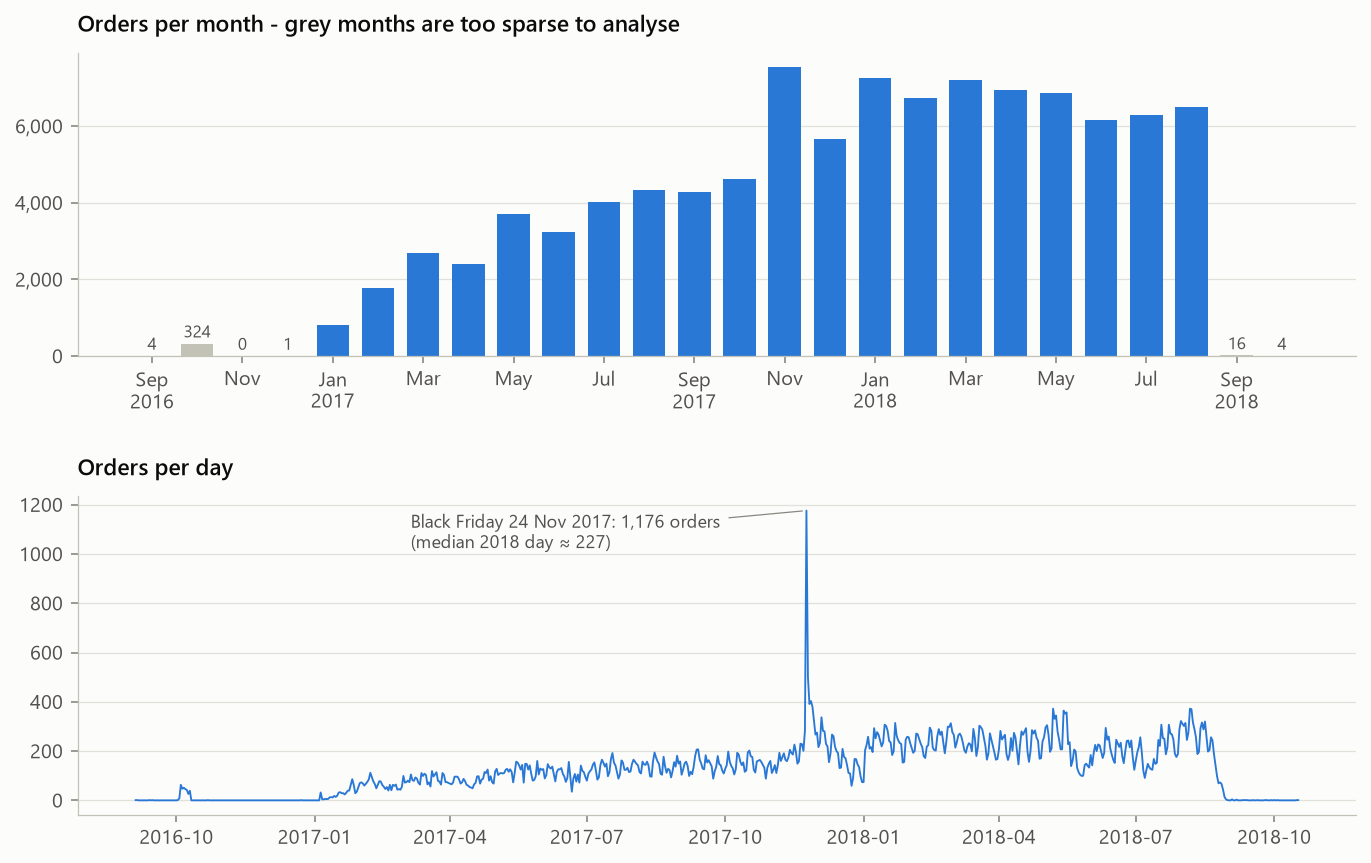
\includegraphics[width=\linewidth]{eda/01_coverage}
  \caption{Số đơn Olist theo tháng và theo ngày}
  \label{fig:eda-coverage}
\end{figure}

Hành vi vận hành cũng không đứng yên theo thời gian (Hình~\ref{fig:eda-operations}, tính theo tháng mua trên các đơn đã giao). Tỉ lệ giao trễ chỉ 3--5\% trong các tháng bình thường nhưng lên 12,4\% với đơn mua tháng 11/2017, 14,1\% với tháng 2/2018 và 19,0\% với tháng 3/2018 (vùng tô xám trong hình); điểm đánh giá trung bình giảm tương ứng xuống 3,91, 3,83 và 3,75, so với khoảng 4,2 ở các tháng khác. Thời gian giao dự kiến (trung vị) giảm từ 39 ngày vào tháng 1/2017 xuống khoảng 23 ngày từ giữa năm 2017 và còn 13,4 ngày vào tháng 8/2018. Cuộc đình công của tài xế xe tải cuối tháng 5/2018 kéo số đơn giao mỗi tuần từ khoảng 2\,000 xuống 634, và số người bán hoạt động mỗi tháng tăng từ 227 lên 1\,278. Những thay đổi chế độ vận hành này là bằng chứng trực tiếp cho lựa chọn chia dữ liệu theo thời gian thay vì chia ngẫu nhiên ở Chương~\ref{ch:method}, bởi một phép chia ngẫu nhiên sẽ trộn các giai đoạn có quy tắc hứa giao và tỉ lệ trễ rất khác nhau.

\begin{figure}[htbp]\centering
  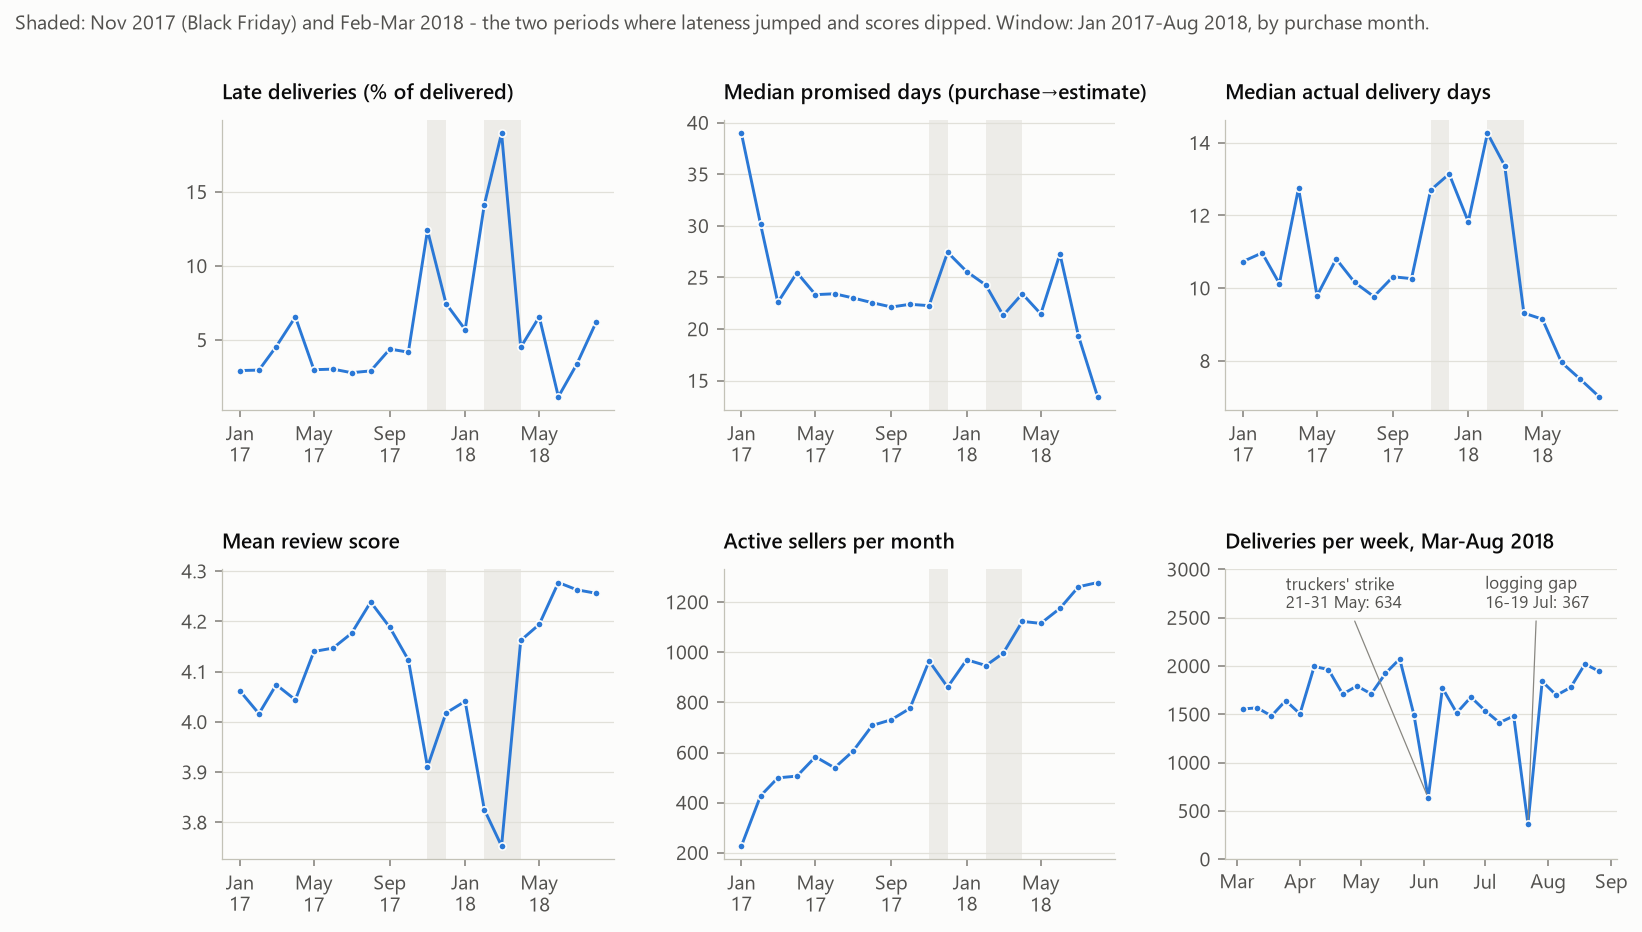
\includegraphics[width=\linewidth]{eda/03_operations_over_time}
  \caption{Diễn biến vận hành theo tháng mua}
  \label{fig:eda-operations}
\end{figure}

Kiểm tra chất lượng dữ liệu cho thấy bộ Olist nhìn chung sạch, nhưng có một số bẫy ảnh hưởng trực tiếp đến cách dựng quần thể. Nếu nối thẳng bảng đơn với bảng sản phẩm, thanh toán và đánh giá mà không gộp trước, kết quả có 117\,329 dòng cho 97\,916 đơn và doanh thu sản phẩm bị đếm thành 14,14 triệu real thay vì 13,59 triệu, đúng hiện tượng nhân bản dòng đã nêu ở Chương~\ref{ch:method}. Có 547 đơn mang 2--3 đánh giá, trong đó 202 đơn có các điểm số không thống nhất, nên cần một luật chọn đánh giá tất định như mô tả ở Chương~\ref{ch:method}; ngoài ra 789 mã đánh giá được dùng chung cho nhiều đơn, nên không thể khử trùng chỉ theo mã đánh giá.

Các mốc thời gian cũng có điểm bất thường. Có 1\,359 đơn có mốc bàn giao vận chuyển sớm hơn mốc duyệt thanh toán và 23 đơn có mốc giao cho khách sớm hơn mốc bàn giao; các khoảng thời gian âm này cần được đánh dấu thay vì tin tưởng. Hai khoảng 16--19/7/2018 và ngày 20/6/2017 gần như không có đơn được ghi nhận giao dù việc bàn giao vận chuyển vẫn diễn ra bình thường, nhiều khả năng là khoảng trống ghi log. Trong 96\,470 đơn đã giao có ngày giao, ngoài bình luận tùy chọn thì chỉ danh mục sản phẩm (1,41\%), đánh giá (0,67\%) và khoảng cách giữa người bán và khách hàng (0,49\%) có tỉ lệ thiếu đáng kể. Ở các bảng phụ, 610 sản phẩm không có danh mục, 26,2\% số dòng tọa độ là bản trùng hoàn toàn và 42 điểm tọa độ nằm ngoài lãnh thổ Brazil.

\subsection{Phân bố điểm đánh giá và mức mất cân bằng lớp}\label{subsec:eda-labels}

Điểm đánh giá có dạng chữ J quen thuộc (Hình~\ref{fig:eda-reviews}). Trên toàn bộ 99\,224 dòng đánh giá, 57,8\% là 5 sao, 19,3\% là 4 sao, 8,2\% là 3 sao, 3,2\% là 2 sao và 11,5\% là 1 sao. Khách không hài lòng viết bình luận nhiều hơn hẳn, với 77\% đánh giá 1 sao có bình luận so với 31\% ở mức 4 sao. Bình luận dồn ứ ở đúng 200 ký tự (659 bình luận), dấu hiệu văn bản đã bị cắt ngắn.

\begin{figure}[htbp]\centering
  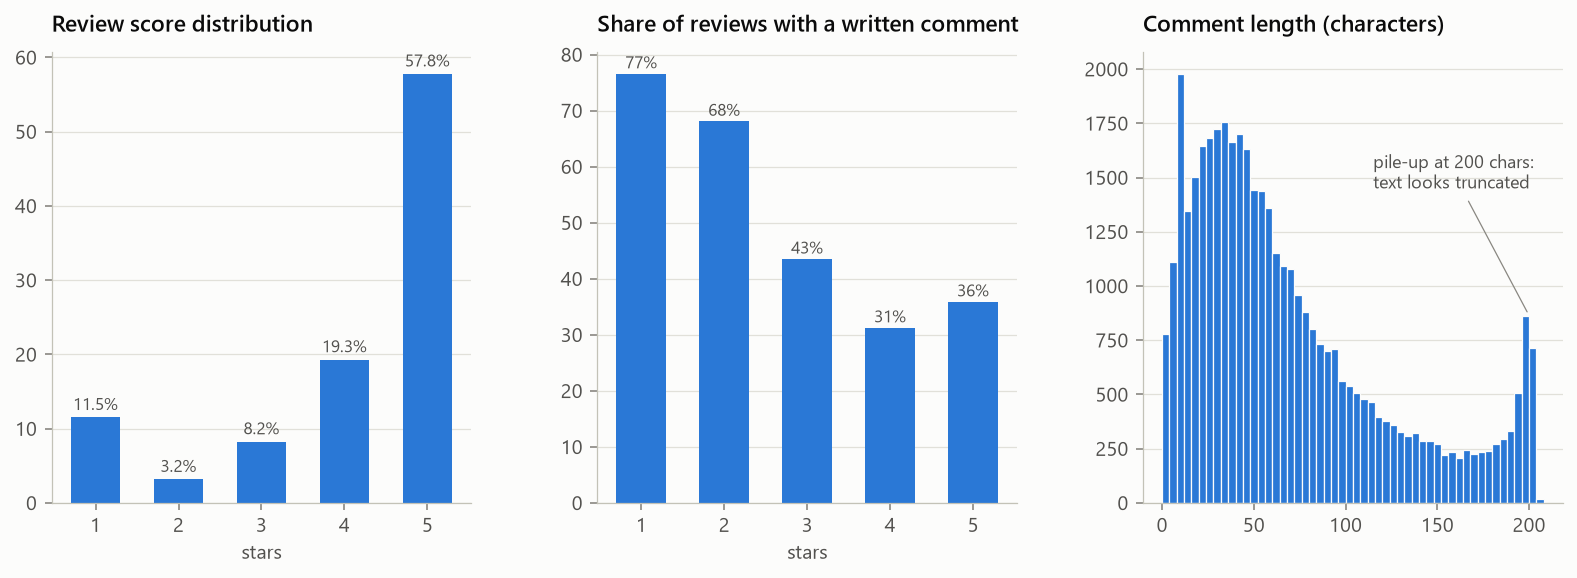
\includegraphics[width=\linewidth]{eda/13_reviews_overview}
  \caption{Phân bố điểm và bình luận đánh giá}
  \label{fig:eda-reviews}
\end{figure}

Trong quần thể nghiên cứu, phân bố dịch về phía hài lòng, với 62,45\% đơn nhận 5 sao, 20,35\% nhận 4 sao, 8,00\% nhận 3 sao, 2,63\% nhận 2 sao và 6,58\% nhận 1 sao. Tỉ lệ dương ở mức đơn vì vậy là 9,21\% (7\,865/85\,420), thấp hơn đáng kể so với 14,69\% khi tính trên mọi đơn có đánh giá. Ở mức item, tỉ lệ dương lên tới 11,41\% vì đơn nhiều sản phẩm có tỉ lệ bị đánh giá thấp cao hơn (mục~\ref{subsec:eda-ontime}) và đóng góp nhiều dòng hơn.

Khác biệt giữa hai mức này cần được ghi nhớ khi đọc Bảng~\ref{tab:split}. Tỉ lệ dương 10,13--13,80\% trong bảng đó được tính ở mức item, còn nếu dựng lại theo cùng mốc thời gian ở mức đơn thì tỉ lệ dương của năm phân vùng phát triển là 8,86--10,53\%. Theo tháng giao, tỉ lệ dương mức đơn của quần thể nghiên cứu dao động trong khoảng 7,8--10,9\%. Với khoảng một đơn dương trên mười một đơn, accuracy không phải thước đo phù hợp, như đã lập luận ở mục~\ref{sec:th-metrics}; tỉ lệ dương mức đơn này cũng là mốc ngẫu nhiên khi đọc PR-AUC ở mục~\ref{sec:results-analysis}.

\subsection{Vì sao giao trễ chi phối các mô hình dự báo hiện có}\label{subsec:eda-lateness}

Một trong những mục tiêu quan trọng của phân tích khám phá là làm rõ vì sao các nghiên cứu dự báo sự hài lòng trên dữ liệu Olist thường xác định giao trễ là yếu tố có ảnh hưởng nổi bật.

Để kiểm tra vấn đề này, nhóm phân tích mẫu gồm 95.824 đơn hàng đã giao và có đánh giá, trong đó tình trạng giao trễ được xác định dựa trên ngày giao thực tế so với ngày dự kiến.

Kết quả cho thấy trên các đơn đã giao có đánh giá, giao trễ là tín hiệu mạnh nhất của đánh giá thấp. Theo định nghĩa trễ theo ngày, 6,7\% đơn bị giao trễ, và nhóm này có 62,4\% đơn bị đánh giá 1--2 sao, gấp 6,7 lần tỉ lệ 9,3\% của đơn đúng hạn. Hình~\ref{fig:eda-factors} đặt tám yếu tố trên cùng một thang đo, với đường xám là tỉ lệ chung 14,7\% trên mọi đơn có đánh giá; các ô về thời gian giao và khoảng cách chỉ tính trên đơn đã giao. Tỉ lệ đánh giá thấp chỉ 9\% với đơn giao sớm từ 7 ngày trở lên và 11\% với đơn giao sớm 0--6 ngày, nhưng lên 32\% khi trễ 1--3 ngày, 68\% khi trễ 4--7 ngày và 79\% khi trễ hơn 7 ngày. Quan hệ này có dạng bậc thang. Giao sớm hơn hứa hẹn hầu như không cải thiện thêm, nhưng chỉ cần vượt qua ngày hứa là tỉ lệ tăng vọt. Theo bảng chi tiết của notebook, tỉ lệ đánh giá thấp là 12,4\% với đơn giao đúng ngày dự kiến, 19,6\% khi trễ một ngày và 50,4\% khi trễ ba ngày. Dạng bất đối xứng này khớp với kết quả của \textcite{ravula2023} và với bằng chứng về tác động của chất lượng giao hàng lên điểm đánh giá~\parencite{deshpande2023}.

\begin{figure}[htbp]\centering
  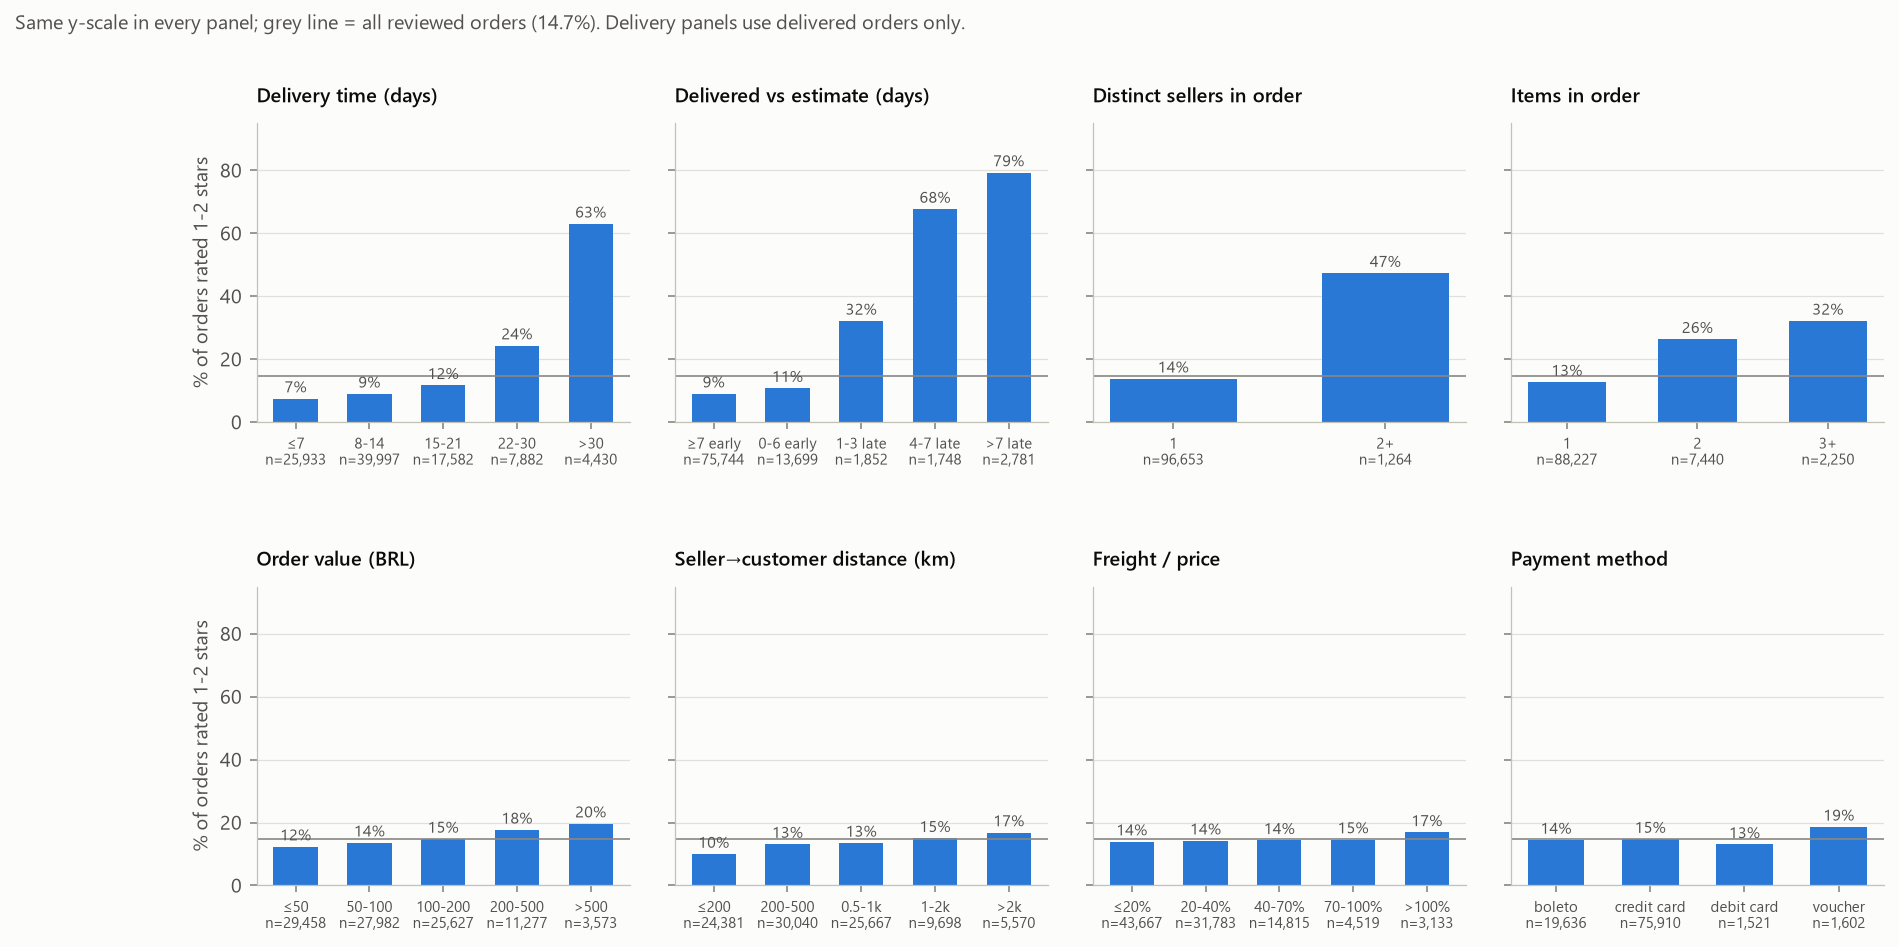
\includegraphics[width=\linewidth]{eda/14_score_factors}
  \caption{Tỉ lệ đánh giá 1--2 sao theo tám yếu tố}
  \label{fig:eda-factors}
\end{figure}

Phân tích trong notebook chỉ ra năm lý do khiến các mô hình hài lòng trên Olist hầu như đều ``phát hiện'' giao trễ là yếu tố quyết định (Bảng~\ref{tab:eda-reasons}). Lý do thứ hai đáng chú ý nhất vì nó nằm ở cơ chế sinh nhãn. Olist gửi khảo sát khi khách nhận hàng \emph{hoặc} khi đến ngày giao dự kiến~\parencite{olist2018}, nên với đơn trễ, khách thường được hỏi về một món hàng chưa nhận được. Trong mẫu đơn trễ, 70,1\% đánh giá được trả lời trước khi hàng đến và 80,8\% số đánh giá này là 1--2 sao; ngược lại, ở đơn đúng hạn chỉ 0,3\% khảo sát được gửi trước ngày giao. Với phần lớn đơn trễ, ``đánh giá'' thực chất là lời phàn nàn hàng chưa tới, và dự báo nó từ mốc thời gian gần như là dự báo lịch gửi khảo sát. Quần thể nghiên cứu loại bỏ vấn đề này từ gốc, vì chỉ giữ đơn giao đúng hạn và có đánh giá tạo sau thời điểm giao.

\begin{table}[htbp]\centering\small
\caption{Năm lý do giao trễ chi phối các mô hình dự báo hài lòng trên Olist (mẫu: 95\,824 đơn đã giao có đánh giá; trễ tính theo ngày)}\label{tab:eda-reasons}
\begin{tabular}{p{4.3cm}p{9.2cm}}
\toprule
Lý do & Bằng chứng \\
\midrule
Giao trễ là tín hiệu mạnh và có dạng bậc thang & 62,4\% đơn trễ bị đánh giá thấp so với 9,3\% đơn đúng hạn; trễ ba ngày đã có 50,4\% đơn bị đánh giá thấp (Hình~\ref{fig:eda-factors}) \\
Nhãn của đơn trễ phần lớn do lịch gửi khảo sát tạo ra & 70,1\% đánh giá của đơn trễ được viết trước khi hàng đến, 80,8\% trong số đó là 1--2 sao \\
Giao trễ quyết định các biến động theo thời gian & Tỉ lệ đánh giá thấp toàn bộ dao động 9,4--21,2\% theo tháng và tăng cùng tỉ lệ trễ (14,0\% tháng 2/2018, 18,7\% tháng 3/2018); tỉ lệ ở đơn đúng hạn chỉ dao động 7,4--10,7\% \\
Đặc trưng thời gian đứng đầu khi gộp mọi đơn & ROC-AUC đơn biến của bốn đặc trưng thời gian đứng đầu là 0,65--0,69 trên mọi đơn, nhưng các đặc trưng này chỉ đạt 0,51--0,57 trên đơn đúng hạn; ở nhóm này số item trong đơn (0,59), tỉ lệ đánh giá thấp trước đó của người bán (0,59) và phí vận chuyển (0,58) dẫn đầu \\
Accuracy che giấu vấn đề & Một mô hình boosting chẩn đoán (chia ngẫu nhiên 70/30, ngưỡng 0,5, như các nghiên cứu trước) đạt accuracy 89,8\%, chỉ hơn mức luôn dự đoán ``không tiêu cực'' (87,2\%) 2,6 điểm; 58,7\% danh sách 10\% rủi ro cao nhất là đơn trễ dù đơn trễ chỉ chiếm 6,7\%, và danh sách này bắt được 96,5\% đơn trễ bị đánh giá thấp nhưng chỉ 16,7\% đơn đúng hạn bị đánh giá thấp \\
\bottomrule
\end{tabular}
\end{table}

Hệ quả là các mô hình huấn luyện trên mọi đơn học chủ yếu cách nhận diện đơn trễ, trong khi phần lớn đánh giá thấp lại nằm ở nhóm còn lại. Trong 12\,272 đơn bị đánh giá 1--2 sao thuộc mẫu đã giao có đánh giá, 8\,289 đơn (67,5\%) đến từ đơn giao đúng hạn theo định nghĩa theo ngày; dùng định nghĩa theo mốc thời gian của quần thể nghiên cứu, con số là 8\,130 đơn (66,25\%). Đơn đúng hạn cũng là trạng thái phổ biến chứ không phải ngoại lệ (Hình~\ref{fig:eda-promise}). Trung vị thời gian giao thực tế là 10,2 ngày so với 23,2 ngày hứa giao, và 93,2\% đơn đến đúng hoặc sớm hạn với trung vị sớm 12 ngày. Theo tháng, tỉ lệ đánh giá thấp của đơn đúng hạn chỉ dao động trong khoảng 7,4--10,7\% (Bảng~\ref{tab:eda-reasons}), nên nhóm khách này không bao giờ hiện lên thành một đỉnh trên biểu đồ vận hành. Đó chính là lý do sự bất mãn của họ được gọi là ``ẩn''.

\begin{figure}[htbp]\centering
  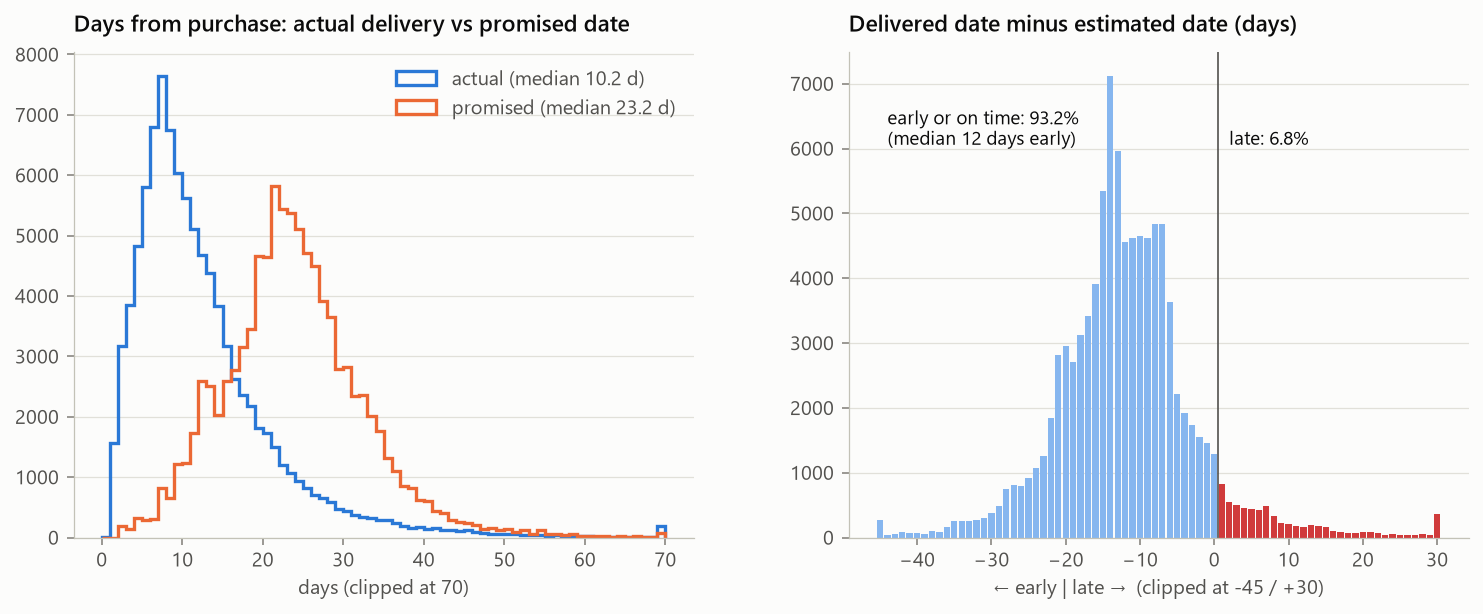
\includegraphics[width=\linewidth]{eda/09_promise_vs_reality}
  \caption{Thời gian giao thực tế so với thời gian hứa giao}
  \label{fig:eda-promise}
\end{figure}

\subsection{Tín hiệu trong nhóm đơn giao đúng hạn}\label{subsec:eda-ontime}

Sau khi xác định mức độ ảnh hưởng của giao trễ, nhóm tiếp tục phân tích riêng quần thể nghiên cứu gồm 85.420 đơn hàng được giao đúng hạn và có đánh giá hợp lệ. Mục tiêu của bước này là tìm kiếm những đặc điểm vẫn có mối liên hệ với đánh giá thấp khi tín hiệu giao trễ đã được loại bỏ.

Khi đã loại giao trễ, các tín hiệu còn lại yếu hơn nhưng không biến mất. Bảng~\ref{tab:eda-segments} tóm tắt tỉ lệ đánh giá thấp mức đơn trong quần thể nghiên cứu theo các yếu tố đều biết được tại thời điểm giao. Cấu trúc đơn tạo khác biệt lớn nhất. Đơn có hai người bán bị đánh giá thấp 45,7\%, gấp hơn năm lần đơn một người bán (8,7\%), và tỉ lệ tăng đều từ 7,5\% ở đơn một item lên 31,9\% ở đơn từ bốn item. Nhóm đơn nhiều người bán rất nhỏ (1\,214 đơn), nhưng tỉ lệ 45,7--63,2\% của nó đã ngang với mức 62,4\% của đơn \emph{trễ} ở mục~\ref{subsec:eda-lateness}. Ở toàn bộ dữ liệu, đơn nhiều người bán còn có tỉ lệ trễ ghi nhận chỉ 1,0\% so với 6,9\% của đơn một người bán và điểm trung bình 2,86 so với 4,12, cho thấy mốc giao duy nhất của đơn nhiều khả năng chỉ phản ánh kiện hàng đến trước. Quan sát này khớp với bằng chứng rằng giao hàng tách kiện làm giảm sự hài lòng~\parencite{brylla2022}.

\begin{table}[htbp]\centering\small
\caption{Tỉ lệ đơn bị đánh giá 1--2 sao trong quần thể nghiên cứu theo một số yếu tố biết được tại thời điểm giao (85\,420 đơn dựng lại; tỉ lệ chung 9,21\%; mỗi yếu tố chỉ trình bày một số nhóm tiêu biểu)}\label{tab:eda-segments}
\begin{tabular}{llrr}
\toprule
Yếu tố & Nhóm & Số đơn & Tỉ lệ đánh giá thấp \\
\midrule
Số người bán trong đơn & 1 & 84\,206 & 8,7\% \\
 & 2 & 1\,157 & 45,7\% \\
 & 3 trở lên & 57 & 63,2\% \\
\addlinespace
Số item trong đơn & 1 & 76\,678 & 7,5\% \\
 & 2 & 6\,695 & 23,2\% \\
 & 3 & 1\,191 & 27,0\% \\
 & 4 trở lên & 856 & 31,9\% \\
\addlinespace
Số ngày từ mua đến giao & $\le$3 & 4\,622 & 6,6\% \\
 & 7--14 & 38\,328 & 8,7\% \\
 & 21--30 & 5\,164 & 14,6\% \\
 & $>$30 & 786 & 22,4\% \\
\addlinespace
Số ngày giao sớm so với dự kiến & 0--3 & 4\,505 & 11,3\% \\
 & 14--21 & 23\,515 & 8,3\% \\
 & $>$30 & 2\,256 & 11,0\% \\
\addlinespace
Bàn giao vận chuyển sau hạn & Không & 79\,118 & 8,9\% \\
 & Có & 6\,302 & 13,6\% \\
\addlinespace
Giá trị sản phẩm (real) & $\le$50 & 25\,911 & 7,8\% \\
 & $>$500 & 3\,020 & 12,9\% \\
\addlinespace
Phí vận chuyển / giá & $\le$20\% & 38\,050 & 8,8\% \\
 & $>$100\% & 2\,663 & 10,6\% \\
\addlinespace
Thanh toán đầu tiên & Thẻ tín dụng & 65\,863 & 9,2\% \\
 & Boleto & 16\,904 & 9,2\% \\
 & Voucher & 1\,342 & 10,5\% \\
\bottomrule
\end{tabular}
\end{table}

Đúng hạn không đồng nghĩa với nhanh. Đơn giao trong vòng ba ngày bị đánh giá thấp 6,6\%, còn đơn mất hơn 30 ngày dù vẫn kịp hạn có tỉ lệ 22,4\%. Khách đánh giá cả độ dài thời gian chờ chứ không chỉ việc lời hứa có được giữ hay không. Khoảng dư so với ngày dự kiến lại có dạng chữ U. Đơn kịp hạn sát nút (0--3 ngày) có tỉ lệ 11,3\%, đơn sớm 14--21 ngày có tỉ lệ thấp nhất 8,3\%, và đơn sớm hơn 30 ngày tăng trở lại 11,0\%, nhiều khả năng vì những đơn này đi kèm thời hạn hứa giao rất dài. Người bán bàn giao vận chuyển sau hạn gửi hàng nhưng hàng vẫn đến kịp có tỉ lệ 13,6\%, so với 8,9\% ở trường hợp còn lại. Lịch sử của người bán cũng mang tín hiệu. Trên mẫu đơn đúng hạn theo ngày của notebook (89\,443 đơn), người bán có hơn 30\% đánh giá thấp trong quá khứ tạo ra 18,4\% đánh giá thấp, so với 6,5\% ở người bán có tỉ lệ quá khứ từ 5\% trở xuống; tỉ lệ quá khứ này chỉ tính trên các đánh giá đã có trước thời điểm mua.

Danh mục sản phẩm tạo khác biệt vừa phải. Tính ở mức item trong quần thể nghiên cứu với các danh mục có từ 800 item, nội thất văn phòng có tỉ lệ dương cao nhất (22,4\% trên 1\,460 item), tiếp theo là đồ trang trí nội thất (14,9\%), chăn ga gối (14,8\%) và phụ kiện máy tính (14,0\%); thấp nhất là phụ kiện hành lý (6,5\%) và văn phòng phẩm (7,6\%). Các item thiếu danh mục có tỉ lệ 15,1\% (1\,344 item), vì vậy giữ ``thiếu danh mục'' thành một nhóm riêng có lợi hơn là điền giá trị. Các yếu tố tiền tệ dịch chuyển ít hơn. Tỉ lệ tăng từ 7,8\% ở đơn dưới 50 real lên 12,9\% ở đơn trên 500 real, còn tỉ trọng phí vận chuyển (8,8--10,6\%) và phương thức thanh toán (8,5--10,5\%) gần như phẳng. Theo bang của khách (các bang có từ 1\,000 đơn), tỉ lệ dao động từ 8,6\% ở São Paulo đến 10,9\% ở Rio de Janeiro và 11,1\% ở Bahia.

Ma trận tương quan Spearman trên 96\,470 đơn đã giao cho thấy vì sao các tín hiệu này khó nắm bắt bằng quan hệ tuyến tính. Không biến số mức đơn nào có hệ số tương quan Spearman với điểm đánh giá vượt quá 0,25 về độ lớn; mạnh nhất là số ngày giao ($-0{,}23$), thời gian vận chuyển ($-0{,}19$), chênh lệch so với ngày dự kiến ($-0{,}18$) và số item ($-0{,}11$). Các quan hệ ở Bảng~\ref{tab:eda-segments} có dạng ngưỡng hoặc chữ U, điều mà tương quan đơn điệu đánh giá thấp. Nhiều cặp biến giải thích lại đi cùng nhau, như số ngày giao và thời gian vận chuyển ($0{,}89$), giá trị đơn và tỉ trọng phí vận chuyển ($-0{,}78$), khoảng cách và số ngày hứa giao ($0{,}62$). Mô hình tuyến tính vì thế dễ gặp đa cộng tuyến, còn mô hình cây có thể tách các ngưỡng mà không cần chỉ định trước dạng quan hệ.

Nhìn chung, kết quả phân tích nhóm đơn giao đúng hạn cho thấy vẫn tồn tại những tín hiệu có thể phục vụ dự báo, đặc biệt là cấu trúc đơn hàng, thời gian giao thực tế và lịch sử vận hành của người bán. Tuy nhiên, các mối liên hệ này cần được kiểm chứng bằng thực nghiệm học máy trước khi kết luận về giá trị dự báo.

\subsection{Nội dung đánh giá của khách không hài lòng}\label{subsec:eda-text}

Bên cạnh những đặc điểm có sẵn tại thời điểm giao hàng, nhóm tiếp tục phân tích nội dung bình luận nhằm hiểu rõ hơn những vấn đề mà khách hàng phản ánh khi để lại đánh giá thấp. Cần nhấn mạnh rằng văn bản đánh giá chỉ xuất hiện sau khi khách hàng phản hồi, nên không được sử dụng làm đặc trưng đầu vào cho mô hình. Trong nghiên cứu này, nội dung bình luận chỉ phục vụ mục đích diễn giải nhãn và tìm hiểu những dạng trải nghiệm tiêu cực có thể tồn tại trong dữ liệu.

Văn bản đánh giá chỉ xuất hiện \emph{sau} khi khách đánh giá, nên nó không được dùng làm đặc trưng (Hình~\ref{fig:leakage-timeline}); nhóm chỉ dùng nó để hiểu nhãn. Theo luật từ khóa trên bình luận tiếng Bồ Đào Nha đã bỏ dấu (Hình~\ref{fig:eda-themes}), bình luận 1 sao chủ yếu nói hàng chưa tới (31\%), sau đó là hoàn tiền, trả hàng hoặc hủy đơn (10\%), thiếu một phần đơn (9\%), giao chậm (7\%), lỗi hoặc hư hỏng (6\%) và giao sai sản phẩm (6\%). Bình luận 4--5 sao thì xoay quanh giao nhanh và lời khen. Bình luận của đơn nhiều người bán khác hẳn, với 31,3\% nói thiếu một phần đơn và 29,8\% nói chưa nhận được hàng, so với 3,0\% và 8,3\% ở đơn một người bán.

Kết quả này bổ sung một góc nhìn quan trọng cho những khác biệt đã quan sát ở mục 4.1.4. Những đơn có nhiều người bán không chỉ có tỷ lệ đánh giá thấp cao hơn mà còn thường xuất hiện các phản hồi liên quan đến việc nhận hàng không đầy đủ.

\begin{figure}[htbp]\centering
  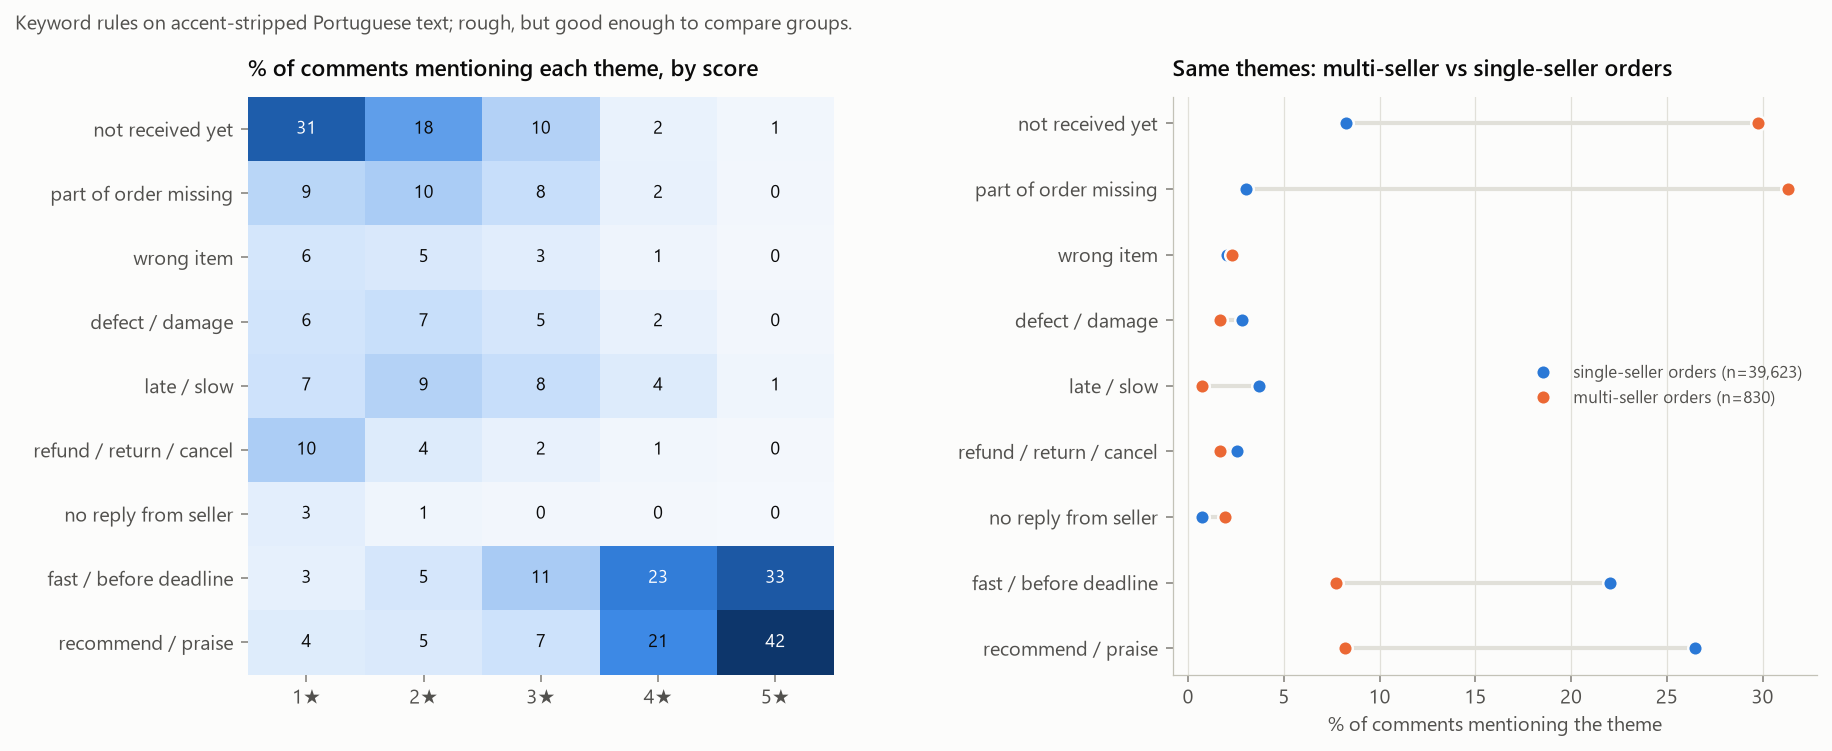
\includegraphics[width=\linewidth]{eda/15_text_themes}
  \caption{Chủ đề trong bình luận đánh giá}
  \label{fig:eda-themes}
\end{figure}

Để làm rõ hơn bản chất của bất mãn ẩn, nhóm so sánh nội dung bình luận tiêu cực giữa đơn giao trễ và đơn giao đúng hạn. Trong 2\,747 bình luận 1--2 sao của đơn trễ, 52,4\% nói chưa nhận được hàng và chỉ 2,0\% nói hàng sai, khác mô tả, lỗi hoặc vỡ. Trong 6\,487 bình luận 1--2 sao của đơn đúng hạn, hai tỉ lệ này lần lượt là 13,9\% và 17,9\%, và 20,3\% nói chỉ nhận được một phần đơn; riêng đơn đúng hạn có từ hai người bán, tỉ lệ nói thiếu một phần lên 51,9\%. Có 78,3\% đánh giá thấp của đơn đúng hạn kèm bình luận. Nói cách khác, khách phàn nàn về đơn trễ vì hàng \emph{chưa đến}, còn khách phàn nàn về đơn đúng hạn vì \emph{thứ đã đến} bị thiếu, sai, hỏng hoặc kém chất lượng. Không vấn đề nào trong số này lộ ra qua chênh lệch giữa ngày giao và ngày dự kiến.

Từ những kết quả trên, có thể nhận thấy sự khác biệt giữa hai nhóm đơn hàng. Với đơn giao trễ, phản hồi tiêu cực chủ yếu liên quan đến việc sản phẩm chưa đến tay khách hàng. Trong khi đó, ở nhóm giao đúng hạn, những vấn đề được phản ánh đa dạng hơn, bao gồm thiếu sản phẩm, giao sai hàng, sản phẩm hư hỏng hoặc chất lượng không đáp ứng kỳ vọng.

Những vấn đề này không thể được nhận diện chỉ bằng cách so sánh thời điểm giao thực tế với ngày giao dự kiến. Vì vậy, phân tích bình luận tiếp tục củng cố giả thuyết rằng việc dự báo bất mãn ẩn cần khai thác những thông tin khác về sản phẩm, cấu trúc đơn hàng và quá trình vận hành.

Tuy nhiên, do phương pháp phân loại bình luận dựa trên từ khóa, kết quả chỉ mang tính mô tả các chủ đề được nhận diện, không phải một hệ thống xác định nguyên nhân đầy đủ cho từng đánh giá.

\subsection{Hàm ý cho thiết kế đặc trưng}\label{subsec:eda-implications}

Những kết quả từ phân tích khám phá dữ liệu không chỉ giúp mô tả hiện tượng bất mãn ẩn mà còn cung cấp cơ sở thực nghiệm cho việc xây dựng các nhóm đặc trưng đã trình bày ở Bảng ~\ref{tab:features}. Trước hết, cấu trúc đơn hàng là nhóm thể hiện sự khác biệt rõ rệt nhất về tỷ lệ đánh giá thấp. Vì vậy, nhóm xây dựng các đặc trưng phản ánh số lượng sản phẩm, số người bán, số danh mục, các cờ đánh dấu đơn nhiều sản phẩm hoặc nhiều người bán, cùng những chỉ số tập trung Herfindahl–Hirschman.
 
Do dữ liệu Olist chỉ ghi nhận một thời điểm giao cho mỗi đơn, những đặc trưng này được sử dụng như các chỉ báo gián tiếp về độ phức tạp của đơn hàng và khả năng phát sinh vấn đề trong quá trình giao nhận. Tuy nhiên, chúng không được xem là bằng chứng xác định một đơn đã bị giao thiếu hoặc chia thành nhiều kiện.

Tiếp theo, nhóm giữ lại những đặc trưng về thời gian giao thực tế, thời gian vận chuyển và khoảng dư so với ngày dự kiến. Kết quả phân tích cho thấy ngay cả khi đơn được giao đúng hạn, thời gian chờ quá dài vẫn có thể đi kèm tỷ lệ đánh giá thấp cao hơn.

Đồng thời, mối quan hệ dạng chữ U của khoảng thời gian giao sớm cho thấy tác động của các biến thời gian không nhất thiết tuyến tính. Đây là một lý do để nhóm ưu tiên thử nghiệm các thuật toán dựa trên cây, vốn có khả năng học những quan hệ dạng ngưỡng và tương tác giữa các biến.

Đối với người bán, nhóm xây dựng các đặc trưng về lịch sử đánh giá, tốc độ xử lý đơn và độ biến động trong hoạt động vận chuyển. Những đặc trưng này hướng đến các tín hiệu đã được quan sát, chẳng hạn người bán có lịch sử đánh giá thấp hoặc thường xuyên bàn giao đơn cho đơn vị vận chuyển sau thời hạn. Tất cả đặc trưng lịch sử đều phải tuân thủ ranh giới thời gian đã trình bày ở Hình~\ref{fig:leakage-timeline}. Danh mục được giữ ở dạng biến phân loại kèm nhóm ``thiếu''. Các nhóm hình thái sản phẩm và độ đầy đủ nội dung nhắm đến các lời phàn nàn về hư hỏng và hàng khác mô tả. Phí vận chuyển, giá trị đơn và thanh toán chỉ cho tín hiệu yếu ở bước khám phá; chúng vẫn nằm trong nhóm cơ sở, nhưng không nên kỳ vọng đóng góp lớn từ riêng các biến này. Ngược lại, văn bản, tiêu đề, thời điểm tạo và thời điểm trả lời đánh giá bị loại khỏi tập đặc trưng, vì đó là thông tin chỉ có sau khi nhãn đã hình thành. Vì vậy, ở mục ~\ref{sec:analysis-eda}, nhóm sẽ đối chiếu các kết quả phân tích khám phá với kết quả lựa chọn đặc trưng của mô hình, nhằm đánh giá mức độ nhất quán giữa những tín hiệu quan sát được và khả năng dự báo thực tế.

% =====================================================================
\section{Kết quả đạt được}\label{sec:results}
Sau khi hoàn tất quá trình phân tích khám phá dữ liệu, nhóm tiến hành thực nghiệm học máy và xây dựng ứng dụng hỗ trợ hoạt động chăm sóc khách hàng. Kết quả của đề tài được thể hiện trên hai phương diện: khả năng tạo ra điểm rủi ro từ dữ liệu đơn hàng và khả năng đưa điểm số đó vào một quy trình vận hành có thể theo dõi, kiểm tra và quản lý.

Tuy nhiên, cần phân biệt giữa kết quả thực nghiệm trong giai đoạn phát triển và kết quả đã được xác nhận trên dữ liệu hoàn toàn độc lập. Những chỉ số học máy hiện có mới phản ánh khả năng dự báo trong phạm vi các fold phát triển, trong khi ứng dụng vận hành sử dụng dữ liệu minh họa để kiểm tra quy trình xử lý.
\subsection{Các thành phần đã hoàn thành}\label{subsec:res-summary}

Quá trình thực nghiệm đã xây dựng được một pipeline xử lý dữ liệu từ các tệp nguồn đến điểm rủi ro ở cấp đơn hàng. Pipeline bao gồm các bước nạp dữ liệu, chuẩn hóa, xây dựng đặc trưng, huấn luyện, đánh giá, hiệu chỉnh xác suất và tổng hợp kết quả dự báo. Bảng~\ref{tab:res-summary} tóm tắt các thành phần chính. 

Sau các giai đoạn thử nghiệm, nhóm giữ lại mô hình Random Forest gồm 200 cây, với độ sâu tối đa bằng 8 và tối thiểu 5 mẫu tại mỗi nút lá. Mô hình sử dụng trọng số lớp cân bằng được tính lại trên từng mẫu bootstrap và chế độ huấn luyện order-weight, trong đó trọng số của mỗi sản phẩm bằng nghịch đảo số sản phẩm thuộc cùng đơn hàng. Cách thiết lập này giúp mỗi đơn hàng đóng góp tổng trọng số tương đương nhau trong quá trình học, đồng thời vẫn khai thác được những thông tin chi tiết ở cấp sản phẩm.

Tập đặc trưng cuối cùng gồm 61 đặc trưng thuộc bảy nhóm ở Bảng~\ref{tab:features}, là kết quả của mười giai đoạn thử nghiệm có kiểm soát. Trong chín giai đoạn đầu, nhóm lần lượt bổ sung những nhóm đặc trưng ứng viên và chỉ giữ lại khi chúng tạo ra mức cải thiện đạt tiêu chí đối với PR-AUC ở cấp đơn hàng, tính trung bình qua ba fold rolling-origin. Ở giai đoạn cuối, nhóm kiểm tra lại các nhóm đã được giữ bằng cách lần lượt loại bỏ từng nhóm, nhằm xác định liệu chúng có tiếp tục đóng góp vào hiệu năng của mô hình khi kết hợp với các đặc trưng khác hay không.

\begin{table}[htbp]\centering\small
\caption{Tóm tắt kết quả thực nghiệm (kết quả phát triển, mang tính thăm dò)}\label{tab:res-summary}
\begin{tabular}{L{3.6cm}L{9.9cm}}
\toprule
Thành phần & Kết quả \\
\midrule
Dữ liệu mô hình hóa & Snapshot đóng băng 85\,425 đơn, 97\,884 item \\
Tập đặc trưng & 61 đặc trưng, 7 nhóm: nhóm cơ sở và các nhóm từ 3 giai đoạn thử nghiệm được giữ \\
Mô hình giữ lại & Rừng ngẫu nhiên, độ sâu 8, lá tối thiểu 5, chế độ order-weight \\
Hiệu chỉnh & Sigmoid; Brier mức item trên phân vùng so sánh giảm từ 0,2203 xuống 0,1049 \\
Ngưỡng ưu tiên & Top 5\% đơn là \textsc{Cao}, top 20\% là \textsc{Trung bình} trở lên \\
PR-AUC mức đơn & 0,1465 (trung bình ba fold; mô hình ban đầu 0,1363) \\
Recall@5\% & 0,1212 (trung bình ba fold; mốc chọn ngẫu nhiên 0,05) \\
Brier mức đơn chưa hiệu chỉnh & 0,1907 (trung bình ba fold; mô hình ban đầu 0,2018) \\
\bottomrule
\end{tabular}
\end{table}

So với mô hình ban đầu cùng họ và cùng chế độ huấn luyện nhưng chỉ dùng nhóm đặc trưng cơ sở, PR-AUC mức đơn trung bình tăng 0,0102 (khoảng 7,5\%) và Brier score giảm 0,0112. Mục tiêu dừng PR-AUC 0,25 của kế hoạch cải thiện không đạt; kế hoạch kết thúc khi các thử nghiệm tiếp theo, kể cả ba cấu hình CatBoost chạy trên GPU và chế độ gộp item thành đơn trước khi huấn luyện, không vượt được mô hình đã giữ trên chỉ số chính.

Điều này cho thấy việc bổ sung thuật toán hoặc đặc trưng phức tạp hơn chưa tạo ra mức cải thiện đủ rõ rệt trong phạm vi thử nghiệm hiện tại. Vì vậy, nhóm giữ lại mô hình Random Forest theo quy tắc lựa chọn đã xác định, đồng thời xem mức hiệu năng còn hạn chế là một kết quả cần tiếp tục phân tích ở các mục sau.

\subsection{Hệ thống hỗ trợ vận hành}\label{sec:system-api}

Bên cạnh mô hình học máy, nhóm xây dựng một ứng dụng hỗ trợ đưa điểm rủi ro vào quy trình chăm sóc khách hàng. Mục tiêu của ứng dụng là giúp nhân viên tiếp cận danh sách đơn hàng theo mức độ ưu tiên, ghi nhận quá trình xử lý và cung cấp thông tin để quản lý theo dõi hoạt động (kiến trúc ở Hình~
ef{fig:arch}).

Hệ thống được tổ chức thành hai luồng hoạt động độc lập. Luồng ngoại tuyến nạp dữ liệu, tạo đặc trưng, huấn luyện và chấm điểm theo lô. Luồng trực tuyến chỉ đọc snapshot điểm đã được ghi để tạo hàng đợi, phân công và ghi nhận xử lý. Việc tách hai luồng loại trừ một rủi ro cơ bản: một thao tác trên giao diện không được làm thay đổi dữ liệu, ngưỡng hay phiên bản mô hình.

PostgreSQL lưu kho dữ liệu Bronze/Silver/Gold, schema \texttt{ml} lưu release, snapshot và ngưỡng, còn schema \texttt{app} lưu case và lịch sử xử lý. Snapshot là điểm nối giữa hai phần. Nó ghi score, phiên bản model, phiên bản ngưỡng, thời điểm chấm điểm và nguồn dữ liệu. Case có thể thay đổi người phụ trách hoặc trạng thái; score và mức rủi ro của snapshot không được sửa qua API. Vì vậy, một quyết định sau này luôn có thể được đối chiếu với thông tin đã có khi hàng đợi được tạo.

API dùng Bearer JWT, còn kiểm soát quyền được thực hiện ở backend. \texttt{SPECIALIST} xem hàng đợi, nhận các case thấp/trung bình hợp lệ và ghi liên lạc. \texttt{MANAGER} phân công case HIGH, mở lại case, đặt quyết định, xem audit và thay đổi tham số. Sự phân vai này không chứng minh hiệu quả CSKH; nó chỉ xác định ai được phép thực hiện bước nào trong quy trình.

Case đi qua \texttt{PENDING}, \texttt{IN\_PROGRESS}, \texttt{COMPLETED} hoặc \texttt{SKIPPED}. Specialist không thể nhận case đã có người xử lý, case HIGH hoặc case vượt năng lực. Khi case được đóng hoặc mở lại, backend tạo và kiểm tra giao dịch thay vì để giao diện tự suy diễn trạng thái. Contact, comment, decision và parameter version được ghi thêm thay vì ghi đè; audit event ghi lại thay đổi workflow. Các quy tắc này phục vụ khả năng kiểm tra, không phải là một lớp trang trí cho giao diện.

Các endpoint dưới tiền tố \texttt{/api/v1} phản ánh các ranh giới trên: \texttt{/auth} cho phiên làm việc; \texttt{/orders} cho hàng đợi và nhận case; \texttt{/contacts}, \texttt{/comments}, \texttt{/decisions} cho bằng chứng xử lý; \texttt{/dashboard}, \texttt{/audit-events} và \texttt{/parameters} cho giám sát. Theo mặc định, hàng đợi được sắp xếp theo điểm rủi ro giảm dần, sau đó xét đến thời hạn SLA và thời gian chờ. Vì vậy, điểm số của mô hình được sử dụng để xác định thứ tự cần kiểm tra, chứ không tự động kết luận khách hàng không hài lòng hoặc tự thực hiện liên hệ.

Nhìn chung, hệ thống đã xây dựng được các thành phần cần thiết để chuyển điểm dự báo thành danh sách công việc có thể quản lý. Tuy nhiên, giá trị của quy trình này trong thực tế vẫn cần được kiểm chứng bằng dữ liệu vận hành và kết quả chăm sóc khách hàng.

\subsection{Phạm vi của bằng chứng}\label{subsec:res-scope}

Mặc dù đề tài đã hoàn thành pipeline thực nghiệm và ứng dụng hỗ trợ vận hành, phạm vi bằng chứng hiện có vẫn cần được xác định rõ để tránh diễn giải kết quả vượt quá những gì dữ liệu cho phép.

Trước hết, toàn bộ chỉ số học máy được trình bày trong chương này đều là kết quả từ ba fold rolling-origin thuộc giai đoạn phát triển. Các chỉ số này phản ánh khả năng dự báo của mô hình trong những lần kiểm định đã thực hiện, nhưng chưa phải ước lượng cuối cùng về hiệu năng trên dữ liệu hoàn toàn độc lập.

Theo thiết kế ban đầu, phân vùng test cuối cùng được dành riêng cho bước đánh giá xác nhận. Tuy nhiên, giai đoạn thời gian của phân vùng này đã bị lộ trong quá trình phát triển. Vì vậy, quy trình hiện tại không cho phép sử dụng nó như một tập kiểm tra niêm phong hợp lệ.

Để có kết luận xác nhận, nhóm cần xây dựng một tập holdout thay thế chưa từng được quan sát hoặc sử dụng trong quá trình lựa chọn mô hình. 

Kết quả backtest trên phân vùng test được trình bày ở mục~\ref{subsec:tab-backtest}, gồm chỉ số mức item và mức đơn, khoảng tin cậy bootstrap của PR-AUC mức đơn và mô phỏng ngân sách 5\%, 10\%, 20\%. Các kết quả sau đây vẫn \emph{chưa} được tính: đường cong precision--recall và đường cong hiệu chỉnh, mốc so sánh theo giá trị đơn, và giá trị SHAP. Báo cáo thực nghiệm cũng không ghi ROC-AUC theo fold, Brier mức item theo fold và tỉ lệ dương của từng đoạn kiểm định; nhóm không suy ra các đại lượng này.

Các con số dưới đây vì vậy trả lời câu hỏi ``trong giai đoạn phát triển, mô hình xếp hạng và ước lượng xác suất tốt đến đâu, và mức đó có ổn định qua thời gian không'', chứ chưa phải ước lượng cuối cùng về hiệu năng khi triển khai.

% =====================================================================
\section{Bảng biểu và số liệu}\label{sec:tables}

\subsection{Hiệu năng của mô hình giữ lại theo fold}\label{subsec:tab-folds}

Bảng~\ref{tab:res-folds} trình bày bốn chỉ số của mô hình giữ lại trên từng fold. Cột cuối là hệ số nâng tại ngân sách 5\%, tức Recall@5\% chia cho 0,05, mức recall kỳ vọng khi chọn ngẫu nhiên (công thức~\eqref{eq:th-recallk}). Ba fold có đoạn kiểm định lần lượt bắt đầu ngày 1/6/2017, 18/7/2017 và 24/8/2017 (Hình~\ref{fig:temporal-folds}).

\begin{table}[htbp]\centering\small
\caption{Kết quả của mô hình giữ lại theo fold rolling-origin (rừng ngẫu nhiên, order-weight, chưa hiệu chỉnh)}\label{tab:res-folds}
\begin{tabular}{crrrrr}
\toprule
Fold & PR-AUC item & PR-AUC đơn & Brier đơn & Recall@5\% & Hệ số nâng \\
\midrule
1 & 0,1538 & 0,1425 & 0,1883 & 0,1141 & 2,28 \\
2 & 0,1883 & 0,1507 & 0,1899 & 0,1309 & 2,62 \\
3 & 0,1860 & 0,1463 & 0,1938 & 0,1187 & 2,37 \\
\midrule
Trung bình & 0,1760 & 0,1465 & 0,1907 & 0,1212 & 2,42 \\
\bottomrule
\end{tabular}
\end{table}

Hình~\ref{fig:res-folds} so sánh mô hình giữ lại với mô hình ban đầu trên cùng ba fold. Mô hình giữ lại tốt hơn ở cả ba fold, theo cả PR-AUC mức đơn lẫn Recall@5\%. Mức cải thiện PR-AUC lần lượt là 0,0120, 0,0060 và 0,0125; Recall@5\% tăng 0,0121, 0,0123 và 0,0158.

\begin{figure}[htbp]\centering
\begin{tikzpicture}[x=1cm,y=25cm,font=\footnotesize]
  % y: 0,16 = 4 cm
  \foreach \ox/\ttl in {0/{PR-AUC mức đơn},6.6/{Recall@5\%}} {
    \begin{scope}[xshift=\ox cm]
      \draw (0,0) -- (5.4,0);
      \draw (0,0) -- (0,0.165);
      \foreach \t/\l in {0/0,0.05/{0,05},0.10/{0,10},0.15/{0,15}} {
        \draw (-0.08,\t) -- (0,\t) node[left,font=\scriptsize]{\l};
        \draw[gray!25] (0,\t) -- (5.4,\t);
      }
      \node[font=\small] at (2.7,0.185) {\ttl};
      \foreach \k in {1,2,3} \node[below,font=\scriptsize] at (1.6*\k-0.5,0) {Fold \k};
    \end{scope}
  }
  % PR-AUC mức đơn: ban đầu / giữ lại
  \foreach \k/\a/\b/\la/\lb in {1/0.1305/0.1425/{0,131}/{0,143},2/0.1447/0.1507/{0,145}/{0,151},3/0.1338/0.1463/{0,134}/{0,146}} {
    \fill[gray!45] (1.6*\k-1.0,0) rectangle (1.6*\k-0.52,\a);
    \fill[blue!55] (1.6*\k-0.48,0) rectangle (1.6*\k,\b);
    \node[above,font=\tiny] at (1.6*\k-0.76,\a) {\la};
    \node[above,font=\tiny] at (1.6*\k-0.24,\b) {\lb};
  }
  % Recall@5%: ban đầu / giữ lại
  \begin{scope}[xshift=6.6cm]
    \foreach \k/\a/\b/\la/\lb in {1/0.1019/0.1141/{0,102}/{0,114},2/0.1185/0.1309/{0,119}/{0,131},3/0.1029/0.1187/{0,103}/{0,119}} {
      \fill[gray!45] (1.6*\k-1.0,0) rectangle (1.6*\k-0.52,\a);
      \fill[blue!55] (1.6*\k-0.48,0) rectangle (1.6*\k,\b);
      \node[above,font=\tiny] at (1.6*\k-0.76,\a) {\la};
      \node[above,font=\tiny] at (1.6*\k-0.24,\b) {\lb};
    }
    \draw[red!70!black,dashed] (0,0.05) -- (5.4,0.05);
  \end{scope}
  % chú giải
  \fill[gray!45] (0.4,-0.03) rectangle (0.7,-0.022); \node[right,font=\scriptsize] at (0.7,-0.026) {Mô hình ban đầu (chỉ nhóm cơ sở)};
  \fill[blue!55] (5.8,-0.03) rectangle (6.1,-0.022); \node[right,font=\scriptsize] at (6.1,-0.026) {Mô hình giữ lại};
  \draw[red!70!black,dashed] (8.7,-0.026) -- (9.3,-0.026); \node[right,font=\scriptsize] at (9.3,-0.026) {Chọn ngẫu nhiên 5\%};
\end{tikzpicture}
\caption{PR-AUC mức đơn và Recall@5\% theo fold}
\label{fig:res-folds}
\end{figure}

\subsection{Đóng góp của các nhóm đặc trưng}\label{subsec:tab-features}

Bảng~\ref{tab:res-phases} liệt kê chín giai đoạn thêm nhóm đặc trưng. Ba nhóm được giữ được thêm nối tiếp nhau, nên PR-AUC tăng từ 0,1363 lên 0,1407 sau giai đoạn 2, lên 0,1445 sau giai đoạn 4 và lên 0,1465 sau giai đoạn 6. Sáu nhóm còn lại bị loại vì mức cải thiện tốt nhất không vượt ngưỡng hoặc làm giảm chỉ số. Cả ba nhóm được giữ đều cải thiện PR-AUC ở từng fold riêng lẻ, không chỉ ở giá trị trung bình.

\begin{table}[htbp]\centering\small
\caption{Kết quả các giai đoạn thử nghiệm nhóm đặc trưng (thay đổi PR-AUC mức đơn trung bình ba fold so với tập đang giữ)}\label{tab:res-phases}
\begin{tabular}{clrl}
\toprule
Giai đoạn & Nhóm đặc trưng ứng viên & Thay đổi PR-AUC & Quyết định \\
\midrule
1 & Lịch sử nhãn của người bán và danh mục (làm trơn) & $+0{,}0015$ (tốt nhất) & Loại \\
2 & Tốc độ và độ biến động vận hành của người bán & $+0{,}0044$ & Giữ \\
3 & Địa lý và tuyến vận chuyển & $-0{,}0024$ (tốt nhất) & Loại \\
4 & Cấu trúc đơn: số lượng, tỉ lệ, mức độ tập trung & $+0{,}0038$ & Giữ \\
5 & Hành vi thanh toán & $+0{,}0006$ (tốt nhất) & Loại \\
6 & Hình thái sản phẩm và độ đầy đủ nội dung & $+0{,}0020$ & Giữ \\
7 & Lịch và khối lượng đơn trước đó & $-0{,}0004$ (tốt nhất) & Loại \\
8 & Cờ chất lượng dữ liệu & $-0{,}0024$ & Loại \\
9 & Tương tác có kiểm soát & $-0{,}0005$ & Loại \\
\bottomrule
\end{tabular}
\end{table}

Giai đoạn 10 kiểm tra lại ba nhóm được giữ bằng cách bỏ từng nhóm một (leave-one-group-out). Bảng~\ref{tab:res-loo} cho thấy bỏ nhóm nào cũng làm PR-AUC giảm ít nhất bằng dung sai 0,002 đặt trước, nên tập đặc trưng rút gọn trùng với tập đầy đủ. Nhóm hình thái và nội dung sản phẩm nằm đúng ở ranh giới này. Cột cuối là PR-AUC mức đơn trên phân vùng lựa chọn mô hình (Bảng~\ref{tab:split}), một tập kiểm định đơn lẻ được báo cáo như bằng chứng phụ.

\begin{table}[htbp]\centering\small
\caption{Bỏ từng nhóm đặc trưng khỏi tập giữ lại (trung bình ba fold, trừ cột cuối)}\label{tab:res-loo}
\begin{tabular}{p{5.6cm}rrrr}
\toprule
Tập đặc trưng & PR-AUC đơn & Thay đổi & Brier đơn & PR-AUC lựa chọn \\
\midrule
Đầy đủ (7 nhóm) & 0,1465 & -- & 0,1907 & 0,2108 \\
Bỏ tốc độ và độ biến động người bán & 0,1424 & $-0{,}0042$ & 0,1956 & 0,2113 \\
Bỏ cấu trúc đơn & 0,1415 & $-0{,}0050$ & 0,1902 & 0,1999 \\
Bỏ hình thái và nội dung sản phẩm & 0,1445 & $-0{,}0020$ & 0,1946 & 0,2185 \\
\bottomrule
\end{tabular}
\end{table}

\subsection{So sánh với các cấu hình CatBoost}\label{subsec:tab-catboost}

Bên cạnh Random Forest, nhóm tiếp tục thử nghiệm ba cấu hình CatBoost trên cùng tập đặc trưng và ba fold rolling-origin. CatBoost được lựa chọn vì có khả năng xử lý trực tiếp các biến phân loại và học những tương tác phi tuyến trong dữ liệu dạng bảng. Việc so sánh nhằm kiểm tra liệu một thuật toán boosting phức tạp hơn có mang lại cải thiện đủ lớn để thay thế mô hình Random Forest đã được giữ lại hay không.

Ba cấu hình CatBoost xử lý biến phân loại trực tiếp được chạy trên cùng tập đặc trưng và cùng ba fold (Bảng~\ref{tab:res-catboost}). Kho lưu trữ chỉ giữ số liệu theo fold của rừng ngẫu nhiên và ba cấu hình này; số liệu của mô hình tỉ lệ nền, hồi quy logistic và HistGradientBoosting không còn, nên bảng không phải là bảng xếp hạng đầy đủ năm họ mô hình đã khai báo ở mục~\ref{sec:models}.

\begin{table}[htbp]\centering\small
\caption{Rừng ngẫu nhiên giữ lại so với ba cấu hình CatBoost (chế độ order-weight, cùng tập đặc trưng)}\label{tab:res-catboost}
\begin{tabular}{lrrrr}
\toprule
& \multicolumn{3}{c}{Trung bình ba fold} & Phân vùng lựa chọn \\
\cmidrule(lr){2-4}\cmidrule(lr){5-5}
Mô hình & PR-AUC đơn & Brier đơn & Recall@5\% & PR-AUC đơn \\
\midrule
Rừng ngẫu nhiên, độ sâu 8, lá 5 & \textbf{0,1465} & 0,1907 & 0,1212 & 0,2108 \\
CatBoost, độ sâu 6, L2 $=8$ & 0,1458 & 0,1681 & \textbf{0,1319} & \textbf{0,2239} \\
CatBoost, độ sâu 8 & 0,1357 & 0,1468 & 0,1229 & 0,2004 \\
CatBoost, độ sâu 10, L2 $=8$ & 0,1374 & \textbf{0,1310} & 0,1180 & 0,1986 \\
\bottomrule
\end{tabular}
\end{table}

Theo thứ tự ưu tiên đã định, rừng ngẫu nhiên được giữ vì có PR-AUC trung bình ba fold cao nhất, dù cấu hình CatBoost độ sâu 6 cao hơn trên phân vùng lựa chọn mô hình và ở Recall@5\%. Không có cấu hình nào đạt mức cải thiện ổn định 0,005 cần thiết để ghép thành mô hình kết hợp.

Vì vậy, kết luận lựa chọn mô hình chỉ được đưa ra trong phạm vi những ứng viên có bằng chứng thực nghiệm có thể đối chiếu trực tiếp.

\subsection{Hiệu chỉnh xác suất và ngưỡng ưu tiên}\label{subsec:tab-calibration}
Sau khi lựa chọn mô hình Random Forest, nhóm tiếp tục thực hiện hiệu chỉnh xác suất nhằm giảm sự khác biệt giữa điểm dự báo và tỷ lệ nhãn dương thực tế.

Mô hình giữ lại được huấn luyện lại trên phân vùng huấn luyện và lựa chọn, hai bộ hiệu chỉnh được fit trên phân vùng fit hiệu chỉnh, rồi cả ba phương án được so sánh bằng Brier score trên phân vùng so sánh hiệu chỉnh (Bảng~\ref{tab:res-calibration}). Brier ở bước này được tính trên xác suất mức item, không có trọng số, nên không so sánh trực tiếp được với Brier mức đơn ở Bảng~\ref{tab:res-folds}. Dòng cuối là dự đoán hằng số bằng tỉ lệ dương mức item của phân vùng so sánh (13,80\%), có Brier bằng $\pi(1-\pi)$, được tính thêm làm mốc tham chiếu.

\begin{table}[htbp]\centering\small
\caption{Brier score mức item trên phân vùng so sánh hiệu chỉnh (2/2018--3/2018)}\label{tab:res-calibration}
\begin{tabular}{lr}
\toprule
Phương án & Brier \\
\midrule
Không hiệu chỉnh & 0,2203 \\
Isotonic & 0,1057 \\
Sigmoid (được chọn) & \textbf{0,1049} \\
\midrule
\emph{Tham chiếu:} dự đoán hằng số $\pi = 0{,}138$ & 0,1189 \\
\bottomrule
\end{tabular}
\end{table}

Với ứng viên CatBoost độ sâu 6, bước hiệu chỉnh cũng chọn sigmoid, với Brier 0,1071 trên cùng phân vùng. Ngưỡng ưu tiên theo chính sách phát triển là 5\% đơn có điểm cao nhất cho mức \textsc{Cao} và 20\% cho mức \textsc{Trung bình} trở lên. Trong một lần chạy rừng ngẫu nhiên trước đó, hai ngưỡng này tương ứng với điểm 0,2858 và 0,1119; đây là ngưỡng chọn trên phân vùng chọn ngưỡng, chưa phải kết quả vận hành trên tập test.

Nhìn chung, quá trình hiệu chỉnh cho thấy mô hình có thể cải thiện đáng kể độ tin cậy của xác suất ở cấp sản phẩm. Tuy nhiên, khả năng hiệu chỉnh ở cấp đơn hàng sau khi tổng hợp điểm bằng max--v1 vẫn cần được đánh giá riêng, bởi phép lấy giá trị lớn nhất có thể làm thay đổi phân bố điểm rủi ro.

\subsection{Kết quả backtest trên phân vùng test}\label{subsec:tab-backtest}

Sau khi cố định mô hình, phương pháp hiệu chỉnh, luật max--v1 và các ngưỡng ưu tiên, nhóm chạy backtest trên phân vùng test (6/2018--8/2018, 18\,561 đơn; Bảng~\ref{tab:split}). Bảng~\ref{tab:res-backtest} trình bày các chỉ số ở hai mức. Do giai đoạn này đã được biết đến trong quá trình phát triển (mục~\ref{subsec:res-scope}), toàn bộ kết quả dưới đây chỉ mang tính thăm dò, chưa phải ước lượng xác nhận độc lập.

% TODO: xác nhận ngưỡng phân loại dùng cho Precision/Recall/F1 và điền vào đoạn dưới nếu cần.
\begin{table}[htbp]\centering\small
\caption{Chỉ số backtest trên phân vùng test theo mức item và mức đơn (luật max--v1)}\label{tab:res-backtest}
\begin{tabular}{lrrrrrr}
\toprule
Mức & PR-AUC & ROC-AUC & Brier & Precision & Recall & F1 \\
\midrule
Item & 0,2306 & 0,6945 & 0,0885 & 0,2109 & 0,5272 & 0,3013 \\
Đơn (max--v1) & 0,1835 & 0,6562 & 0,0753 & 0,1857 & 0,3441 & 0,2412 \\
\bottomrule
\end{tabular}
\end{table}

Khoảng tin cậy bootstrap của PR-AUC mức đơn, tính từ 1\,000 lần lấy mẫu lại theo cụm đơn hàng, là $[0{,}1679;\ 0{,}2021]$, rộng khoảng $\pm 0{,}017$ quanh giá trị điểm. PR-AUC chỉ có nghĩa khi đặt cạnh tỉ lệ dương của phân vùng test, vốn được niêm phong và chưa báo cáo (mục~\ref{sec:th-metrics}). Mức item có PR-AUC cao hơn mức đơn (0,2306 so với 0,1835), phù hợp với nhận xét ở mục~\ref{sec:analysis-ranking} rằng tỉ lệ dương mức item cao hơn và các item cùng đơn bị đếm lặp. Con số 0,1835 cũng cao hơn PR-AUC trung bình ba fold (0,1465), nhưng hai con số này tính trên hai giai đoạn có tỉ lệ dương khác nhau nên không so sánh trực tiếp được.

Bảng~\ref{tab:res-budget} mô phỏng việc xem xét theo ngân sách: chọn tỉ lệ đơn có điểm cao nhất rồi đo mức bắt được. Hệ số nâng là Recall chia cho tỉ lệ ngân sách, tức mức recall kỳ vọng khi chọn ngẫu nhiên (công thức~\eqref{eq:th-recallk}).

\begin{table}[htbp]\centering\small
\caption{Mô phỏng ngân sách xem xét trên phân vùng test}\label{tab:res-budget}
\begin{tabular}{rrrrrr}
\toprule
Ngân sách & Đơn được chọn & Precision rủi ro & Recall rủi ro & Hệ số nâng & Giá trị đơn bị đánh giá thấp bắt được \\
\midrule
5\%  &    929 & 0,2896 & 0,1698 & 3,40 & 0,2298 \\
10\% &  1\,857 & 0,2219 & 0,2601 & 2,60 & 0,3465 \\
20\% &  3\,713 & 0,1689 & 0,3958 & 1,98 & 0,4450 \\
\bottomrule
\end{tabular}
\end{table}

Khi ngân sách tăng, Recall tăng nhưng Precision giảm: mở rộng từ 5\% lên 20\% đơn giúp bắt thêm từ 17,0\% lên 39,6\% số đơn bị đánh giá thấp, nhưng tỉ lệ đơn được chọn thực sự bị đánh giá thấp giảm từ 29,0\% xuống 16,9\%. Hệ số nâng giảm dần từ 3,40 xuống 1,98, tức hiệu quả biên của mỗi đơn được xem xét thêm giảm khi ngân sách rộng hơn. Tỉ lệ giá trị đơn bắt được luôn cao hơn Recall (ví dụ 0,2298 so với 0,1698 ở ngân sách 5\%), tức các đơn bị đánh giá thấp được bắt có giá trị trung bình cao hơn các đơn bị đánh giá thấp còn sót lại. Mốc so sánh theo giá trị đơn, vốn là đối thủ chính trong nghiên cứu của \textcite{li2026valuesorting}, chưa được chạy trên cùng phân vùng, nên chưa thể kết luận mô hình có vượt cách sắp xếp theo giá trị hay không.

% =====================================================================
\section{Phân tích và đánh giá}\label{sec:results-analysis}

Những kết quả ở mục 4.3 cho thấy mô hình Random Forest có khả năng nhận diện một phần các đơn hàng giao đúng hạn nhưng có nguy cơ nhận đánh giá thấp. Tuy nhiên, để xác định ý nghĩa của kết quả, cần xem xét không chỉ giá trị các chỉ số mà còn cả mức cải thiện so với mốc tham chiếu, sự ổn định theo thời gian và những giới hạn của phương pháp đánh giá.

Vì vậy, mục này tập trung phân tích bốn vấn đề: khả năng xếp hạng so với lựa chọn ngẫu nhiên, độ ổn định giữa các fold, độ tin cậy của xác suất sau hiệu chỉnh và mức độ nhất quán giữa kết quả mô hình với những phát hiện từ phân tích khám phá dữ liệu.

\subsection{Khả năng xếp hạng so với mốc ngẫu nhiên}\label{sec:analysis-ranking}

Đối với bài toán mất cân bằng lớp, PR-AUC chỉ có nghĩa khi đặt cạnh tỉ lệ dương, vì một mô hình xếp hạng ngẫu nhiên có PR-AUC xấp xỉ tỉ lệ dương (mục~\ref{sec:th-metrics}). Báo cáo thực nghiệm không ghi tỉ lệ dương mức đơn của từng đoạn kiểm định. Nếu tỉ lệ này nằm trong khoảng 8,86--10,53\% như ở các phân vùng phát triển (mục~\ref{subsec:eda-labels}), PR-AUC mức đơn trung bình 0,1465 gấp khoảng 1,4 đến 1,65 lần mốc ngẫu nhiên. Mô hình vì thế học được tín hiệu thật, nhưng tín hiệu đó yếu, vì phần lớn các đơn có điểm cao vẫn là đơn không bị đánh giá thấp.

Ở mức vận hành, Recall@5\% trung bình 0,1212 cho hệ số nâng 2,42, dao động 2,28--2,62 giữa các fold. Nếu bộ phận chăm sóc khách hàng chỉ liên hệ được 5\% số đơn giao đúng hạn, danh sách theo mô hình chứa khoảng 12\% số đơn sẽ bị đánh giá thấp, so với 5\% khi chọn ngẫu nhiên. Từ công thức~\eqref{eq:th-recallk}, $\mathrm{Precision@}b = \mathrm{Recall@}b \cdot \pi / b$; với $\pi$ trong khoảng 8,86--10,53\% như trên, khoảng 21--26\% số đơn được gắn mức \textsc{Cao} thực sự bị đánh giá thấp, tức chừng một trong bốn hoặc năm đơn, so với khoảng một trong mười đơn nếu chọn ngẫu nhiên. Đây là ước tính suy ra, chưa phải số đo trực tiếp.

PR-AUC mức item (0,1760) cao hơn mức đơn (0,1465), nhưng chênh lệch này chủ yếu đến từ mốc so sánh chứ không phải từ chất lượng xếp hạng. Trong quần thể nghiên cứu, tỉ lệ dương mức item là 11,41\%, cao hơn mức đơn 9,21\%, vì đơn nhiều sản phẩm vừa có tỉ lệ đánh giá thấp cao hơn vừa đóng góp nhiều dòng hơn. Chia cho tỉ lệ dương tương ứng của quần thể, cả hai chỉ số đều ở khoảng 1,5--1,6 lần mốc ngẫu nhiên. Ngoài ra, các item trong cùng một đơn dương có đặc trưng mức đơn giống nhau và cùng nhãn, nên PR-AUC mức item được lợi từ việc đếm lặp. Bên cạnh đó, các sản phẩm thuộc cùng một đơn hàng chia sẻ nhiều đặc trưng và cùng nhãn đánh giá, nên việc đánh giá ở cấp item có thể chịu ảnh hưởng từ hiện tượng đếm lặp những đơn nhiều sản phẩm. 

Vì vậy, PR-AUC ở cấp đơn hàng vẫn được xem là chỉ số quan trọng hơn đối với mục tiêu của đề tài, bởi đơn hàng mới là đơn vị mà nhân viên chăm sóc khách hàng thực sự xử lý., đúng như lựa chọn ở mục~\ref{sec:eval}.

\subsection{Độ ổn định qua thời gian và lựa chọn mô hình}\label{sec:analysis-stability}

Bên cạnh khả năng vượt mốc ngẫu nhiên, độ ổn định của kết quả giữa các giai đoạn thời gian cũng là yếu tố cần xem xét.

PR-AUC mức đơn của mô hình giữ lại dao động từ 0,1425 đến 0,1507 giữa ba fold, với độ lệch chuẩn khoảng 0,004. Con số này cho một thang đo để đọc Bảng~\ref{tab:res-phases}. Mỗi nhóm đặc trưng được giữ chỉ cải thiện 0,0020--0,0044, tức xấp xỉ một độ lệch chuẩn giữa các fold. Một mức cải thiện trung bình cỡ đó có thể là nhiễu, và đó là lý do quyết định giữ nhóm còn dựa vào việc nhóm có cải thiện ở từng fold hay không. Mức cải thiện cộng dồn 0,0102 bằng khoảng 2,5 lần độ lệch chuẩn và xuất hiện ở cả ba fold (Hình~\ref{fig:res-folds}), nên đáng tin hơn bất kỳ bước riêng lẻ nào. Fold 1 có PR-AUC mức item thấp nhất (0,1538); đây cũng là fold học trên ít dữ liệu nhất, phù hợp với nhận xét ở mục~\ref{sec:th-temporal}, dù với ba fold thì chưa thể tách tác động của cỡ mẫu khỏi đặc điểm của từng giai đoạn.

Cùng thang đo đó cho thấy rừng ngẫu nhiên và CatBoost độ sâu 6 gần như ngang nhau. Chênh lệch PR-AUC ba fold giữa hai mô hình chỉ là 0,0007, nhỏ hơn nhiều so với độ lệch chuẩn giữa các fold. Ở Recall@5\%, CatBoost độ sâu 6 cao hơn 0,0107 và không kém rừng ngẫu nhiên ở fold nào (0,1408, 0,1309 và 0,1240 so với 0,1141, 0,1309 và 0,1187). Quy tắc chọn theo PR-AUC đã được cố định trước khi chạy và được áp dụng đúng; tuy vậy, kết quả này cho thấy nếu ngân sách 5\% là ràng buộc vận hành chính, Recall@5\% có lý do để trở thành tiêu chí phụ trong lần lựa chọn sau. Trên phân vùng lựa chọn mô hình, thứ hạng hai mô hình đảo ngược (0,2239 so với 0,2108); ý nghĩa của sự đảo ngược này đối với cách đánh giá được bàn ở mục~\ref{sec:disc-findings}.

Kết quả bỏ từng nhóm cũng cho thấy giới hạn của một tập kiểm định đơn lẻ. Bỏ nhóm hình thái và nội dung sản phẩm làm PR-AUC ba fold giảm 0,0020 nhưng làm PR-AUC trên phân vùng lựa chọn \emph{tăng} từ 0,2108 lên 0,2185 (Bảng~\ref{tab:res-loo}). Hai nguồn bằng chứng chỉ ra hai hướng ngược nhau, và nhóm này được giữ có điều kiện theo chỉ số chính. Ngược lại, nhóm cấu trúc đơn hàng có bằng chứng ổn định hơn, bởi việc loại bỏ nhóm này làm giảm kết quả trên cả ba fold trung bình và phân vùng lựa chọn mô hình.

Nhìn chung, mô hình giữ lại có mức cải thiện nhất quán so với mô hình ban đầu, nhưng sự khác biệt giữa những ứng viên cạnh tranh vẫn còn nhỏ. Điều này cho thấy việc lựa chọn mô hình cần được đánh giá thận trọng, đặc biệt khi kết quả chỉ dựa trên một số lượng fold hạn chế.

\subsection{Độ tin cậy của xác suất}\label{sec:analysis-calibration}

Bên cạnh khả năng xếp hạng, độ tin cậy của xác suất là yếu tố quan trọng khi điểm dự báo được đưa vào hệ thống chăm sóc khách hàng.

Trước hiệu chỉnh, xác suất của mô hình kém tin cậy. Brier mức đơn trung bình ba fold là 0,1907, trong khi một dự đoán hằng số bằng tỉ lệ dương mức đơn 8,86--10,53\% cho Brier $\pi(1-\pi)$ khoảng 0,081--0,094. Trên phân vùng so sánh hiệu chỉnh, Brier mức item của mô hình gốc là 0,2203, cao gần gấp đôi mốc hằng số 0,1189. Đây đúng là hệ quả mà mục~\ref{sec:th-trees} đã dự đoán. Trọng số lớp cân bằng làm tỉ lệ dương hiệu dụng trong các lá cao hơn thực tế, nên xác suất bị đẩy lên một cách có hệ thống, phù hợp với kết quả của \textcite{vandengoorbergh2022}. Ba cấu hình CatBoost có Brier ba fold thấp hơn (0,1310--0,1681), cho thấy mức méo phụ thuộc vào mô hình nhưng không biến mất.

Hiệu chỉnh sửa được phần lớn độ lệch này. Sigmoid giảm Brier mức item từ 0,2203 xuống 0,1049, tức giảm 52\%, và đưa mô hình xuống dưới mốc hằng số 0,1189 khoảng 12\%. Isotonic cho kết quả gần như bằng (0,1057). Khi tập fit hiệu chỉnh có 11\,759 đơn, nguy cơ quá khớp của isotonic mà \textcite{niculescumizil2005} cảnh báo không thể hiện rõ; sigmoid được chọn vì Brier thấp hơn và vì nó giữ nguyên hoàn toàn thứ tự xếp hạng (mục~\ref{sec:th-calibration}). Rừng ngẫu nhiên sau hiệu chỉnh cũng nhỉnh hơn CatBoost độ sâu 6 sau hiệu chỉnh (0,1049 so với 0,1071).

Những kết quả này cho thấy bước hiệu chỉnh có thể cải thiện đáng kể chất lượng xác suất ở cấp sản phẩm. Tuy nhiên, vẫn tồn tại một giới hạn quan trọng: Brier score sau hiệu chỉnh ở cấp đơn hàng chưa được báo cáo.

Như đã phân tích ở Chương 2, việc lấy giá trị lớn nhất của nhiều xác suất item theo quy tắc max-v1 có thể khiến điểm tổng hợp ở cấp đơn cao hơn mức rủi ro thực tế, đặc biệt đối với những đơn chứa nhiều sản phẩm.

Vì vậy, dù xác suất ở cấp sản phẩm đã được hiệu chỉnh tốt hơn, chưa thể kết luận điểm tổng hợp ở cấp đơn hàng cũng có độ tin cậy tương tự.

Trong phạm vi hiện tại, điểm rủi ro hiển thị trên ứng dụng nên được hiểu chủ yếu là thông tin phục vụ xếp hạng ưu tiên, thay vì xác suất chính xác rằng một đơn hàng cụ thể sẽ nhận đánh giá thấp.

\subsection{Đối chiếu với kết quả khám phá dữ liệu}\label{sec:analysis-eda}

Một cách khác để đánh giá tính hợp lý của mô hình là đối chiếu những nhóm đặc trưng được giữ lại với các tín hiệu đã quan sát trong quá trình phân tích khám phá dữ liệu ở mục 4.1.

Kết quả chọn đặc trưng khớp với các tín hiệu tìm thấy ở mục~\ref{subsec:eda-ontime}. Nhóm cấu trúc đơn, nơi bước khám phá ghi nhận khác biệt lớn nhất (45,7\% ở đơn hai người bán, 31,9\% ở đơn từ bốn item), là nhóm được giữ có đóng góp lớn nhất khi bỏ ra ($-0{,}0050$). Nhóm vận hành của người bán tương ứng với tín hiệu bàn giao vận chuyển sau hạn (13,6\% so với 8,9\%) và được giữ với mức giảm $-0{,}0042$ khi bỏ. Nhóm sản phẩm tương ứng với khác biệt giữa các danh mục và tỉ lệ cao ở item thiếu danh mục. Ở chiều ngược lại, các yếu tố gần như phẳng ở bước khám phá đều bị loại khi thử nghiệm. Thanh toán (8,5--10,5\% theo phương thức) chỉ cải thiện tốt nhất 0,0006, còn địa lý (8,6--11,1\% theo bang) làm giảm PR-AUC.

Ngoại lệ đáng chú ý là lịch sử nhãn. Bước khám phá cho thấy người bán có tiền sử nhiều đánh giá thấp tạo ra tỉ lệ đánh giá thấp gấp gần ba lần (18,4\% so với 6,5\%), nhưng nhóm lịch sử nhãn làm trơn ở giai đoạn 1 chỉ cải thiện tốt nhất 0,0015 và bị loại. Hai kết quả này không mâu thuẫn, bởi nhóm cơ sở đã có số đánh giá trước đó và điểm trung bình trước đó của người bán và danh mục, nên các phép mã hóa mới chủ yếu lặp lại thông tin đã có. Ý nghĩa của việc đặc trưng vận hành vượt lịch sử đánh giá được thảo luận ở mục~\ref{sec:disc-findings}.

Bước khám phá cũng cho phép đánh giá một phần thiên lệch của luật max-v1. Công thức~\eqref{eq:th-maxbias} dự đoán max-v1 nâng điểm đơn nhiều item ngay cả khi từng item không rủi ro hơn. Trong quần thể nghiên cứu, đơn nhiều item thực sự rủi ro hơn, với tỉ lệ 23,2--31,9\% so với 7,5\% ở đơn một item (Bảng~\ref{tab:eda-segments}). Thiên lệch của max-v1 vì vậy cùng chiều với rủi ro thật, nên nó ít có khả năng đẩy sai đơn lên đầu danh sách. Tuy nhiên, chưa thể biết max-v1 nâng điểm các đơn này vừa đủ hay quá mức, vì dự đoán mức đơn theo số item chưa được lưu lại để kiểm tra.

Nhìn chung, kết quả thực nghiệm tương đối phù hợp với những phát hiện từ phân tích khám phá dữ liệu, đặc biệt đối với cấu trúc đơn hàng và đặc điểm vận hành của người bán. Tuy nhiên, sự nhất quán này chỉ hỗ trợ giải thích giá trị dự báo của các đặc trưng, không chứng minh chúng là nguyên nhân trực tiếp khiến khách hàng không hài lòng.

\subsection{Đánh giá tổng hợp}\label{sec:analysis-summary}

Từ những kết quả đã phân tích, có thể nhận thấy mô hình đáp ứng hai yêu cầu cơ bản trong giai đoạn phát triển, kết quả đáp ứng hai tiêu chí tối thiểu của mục~\ref{sec:eval}. Mô hình xếp hạng tốt hơn ngẫu nhiên ở cả mức đơn lẫn ngân sách 5\%, và mức vượt đó xuất hiện ở cả ba fold chứ không chỉ ở giá trị trung bình. Xác suất sau hiệu chỉnh tốt hơn dự đoán hằng số ở mức item. Ba giới hạn ảnh hưởng trực tiếp đến cách đọc các con số. Thứ nhất, tín hiệu còn yếu, khi PR-AUC chỉ khoảng 1,4--1,65 lần mốc ngẫu nhiên, và khoảng 88\% số đơn bị đánh giá thấp nằm ngoài nhóm 5\% đầu danh sách. Thứ hai, độ chính xác của phép lựa chọn bị giới hạn bởi ba fold; phần lớn chênh lệch giữa các phương án cạnh tranh nhỏ hơn độ dao động giữa các fold. Thứ ba, các kết quả chưa được xác nhận trên tập test niêm phong và chưa có mốc so sánh theo giá trị đơn. Chương~\ref{ch:discussion} đặt các kết quả này cạnh mục tiêu ban đầu và bàn về nguyên nhân của mức tín hiệu thấp; mục tiếp theo trình bày cách điểm rủi ro được dùng trong ứng dụng.

Để chuyển từ kết quả phát triển sang kết luận có độ tin cậy cao hơn, bước tiếp theo cần thực hiện là xây dựng một tập holdout thay thế chưa từng được quan sát. Trước khi đánh giá, nhóm cần cố định mô hình, phương pháp hiệu chỉnh, quy tắc tổng hợp và các ngưỡng ưu tiên, sau đó tính toán những chỉ số cần thiết kèm khoảng tin cậy và lưu lại dữ liệu dự báo để kiểm tra.

Như vậy, kết quả hiện tại cho thấy hướng tiếp cận có tiềm năng hỗ trợ việc ưu tiên chăm sóc khách hàng, nhưng vẫn cần thêm bằng chứng để xác nhận hiệu năng và giá trị khi triển khai thực tế.
 % Chương 4 — mục Ứng dụng điểm rủi ro (Trúc), nạp ngay sau ch4.tex.
% Nguồn: BA/*.md, reports/P13-full-flow-audit-2026-10-31.md, SERVER_CONTEXT/chapter4_evidence.md (nhánh thesis),
% ảnh chụp 05/11/2026 từ stack Docker nhánh dev (commit 1a8a767).
% Phần này trả lời câu hỏi: điểm số của mô hình được đưa vào quy trình chăm sóc khách hàng như thế nào.
% Chia việc Ch.4: Quân (EDA, dữ liệu) · Trung (hệ thống/API) · Huy (bảng metric) · Trúc (giao diện/demo).
% Không lặp kiến trúc/API (phần Trung) và kết quả kiểm thử web (để ở báo cáo kiểm thử, không đưa vào đồ án ML).

\section{Ứng dụng điểm rủi ro vào quy trình chăm sóc khách hàng}\label{sec:demo}

Kết quả học máy chỉ có ý nghĩa đối với hoạt động kinh doanh khi có thể được chuyển thành thông tin hỗ trợ ra quyết định. Trong bài toán của đề tài, điểm rủi ro không được sử dụng để tự động kết luận một khách hàng không hài lòng, mà nhằm giúp bộ phận chăm sóc khách hàng xác định những đơn hàng nên được kiểm tra trước trong điều kiện nguồn lực xử lý có hạn.

Xuất phát từ mục tiêu đó, nhóm xây dựng ứng dụng vận hành để kết nối đầu ra của mô hình với quy trình quản lý đơn hàng. Ứng dụng cho phép tạo danh sách ưu tiên, hiển thị thông tin liên quan đến điểm rủi ro, phân công nhân viên, ghi nhận quá trình liên hệ và theo dõi kết quả xử lý.

Bên cạnh việc hỗ trợ quy trình làm việc, hệ thống còn được thiết kế để lưu trữ dữ liệu vận hành có cấu trúc, tạo tiền đề cho việc đánh giá và cải thiện mô hình trong những giai đoạn tiếp theo.

Tuy nhiên, cần phân biệt rõ giữa ứng dụng minh họa và kết quả thực nghiệm học máy. Bản demo hiện sử dụng 100 đơn hàng Olist thật với thông tin về đơn hàng, người bán và danh mục, kết hợp cùng điểm rủi ro minh họa được tạo theo quy tắc tất định và 5 đơn hàng giả lập. Phiên bản mô hình hiển thị trên giao diện là \texttt{olist-ui-demo-v1}. Lý do và hệ quả của lựa chọn này được phân tích tại mục~\ref{sec:demo-limits}. Do đó, mục này đánh giá cách hệ thống sử dụng điểm số, không đánh giá chất lượng của điểm số.

% ---------------------------------------------------------------------
\subsection{Từ điểm số đến hàng đợi ưu tiên}

Để bảo đảm mô hình học máy và ứng dụng vận hành hoạt động độc lập, nhóm sử dụng bảng dự đoán trong cơ sở dữ liệu làm điểm kết nối giữa hai thành phần.

Giữa luồng học máy và ứng dụng chỉ có một điểm nối là bảng dự đoán trong cơ sở dữ liệu (Hình~\ref{fig:arch}). Mỗi lần chấm điểm theo lô tạo ra một \emph{snapshot dự đoán} bất biến, gồm điểm của từng item, điểm của đơn tổng hợp theo luật max-v1 (Phương trình~\ref{eq:maxv1}), mức rủi ro theo ngưỡng của phiên bản mô hình, các yếu tố liên quan và các mã phiên bản. Tại mỗi thời điểm chỉ một snapshot ở trạng thái hoạt động. Ứng dụng đọc snapshot này để tạo các \emph{case} cần xử lý; mỗi case giữ mã dự đoán và luật tổng hợp tại thời điểm được tạo, nên khi mô hình được chấm lại, các case đang mở vẫn được xử lý theo đúng điểm số đã sinh ra chúng thay vì bị đổi điểm giữa chừng.

Hình~\ref{fig:ui-queue} là hàng đợi rủi ro của nhân viên chăm sóc khách hàng. Ba quyết định thiết kế ở đây xuất phát trực tiếp từ đặc điểm của mô hình:

\begin{itemize}
  \item \textbf{Xếp theo điểm, sau đó theo hạn xử lý.} Đơn được sắp theo điểm rủi ro giảm dần, rồi theo hạn SLA gần nhất và thời gian chờ. Do điểm số chỉ mang ý nghĩa thứ tự (mục~\ref{sec:eval}), giao diện sử dụng điểm số để sắp xếp thay vì chuyển thành nhãn ``sẽ bị đánh giá thấp''.
  \item \textbf{Hiện sản phẩm có điểm cao nhất ngay trên dòng của đơn.} Cột ``Sản phẩm cần kiểm tra'' cho biết item quyết định điểm của đơn theo luật max-v1, kèm số sản phẩm còn lại. Thông tin này giúp nhân viên xác định sản phẩm cần trao đổi với khách hàng trước, đồng thời cho biết nguồn gốc điểm số của đơn.
  \item \textbf{Mức rủi ro quyết định ai xử lý.} Đơn mức cao do quản lý phân công, đơn mức trung bình và thấp nhân viên tự nhận. Vì vậy, ngưỡng rủi ro đóng vai trò quy tắc phân bổ nguồn lực, không chỉ là nhãn hiển thị, phù hợp với lập luận chọn ngưỡng theo năng lực xử lý ở mục~\ref{sec:models}.
\end{itemize}

\begin{figure}[!htbp]\centering
  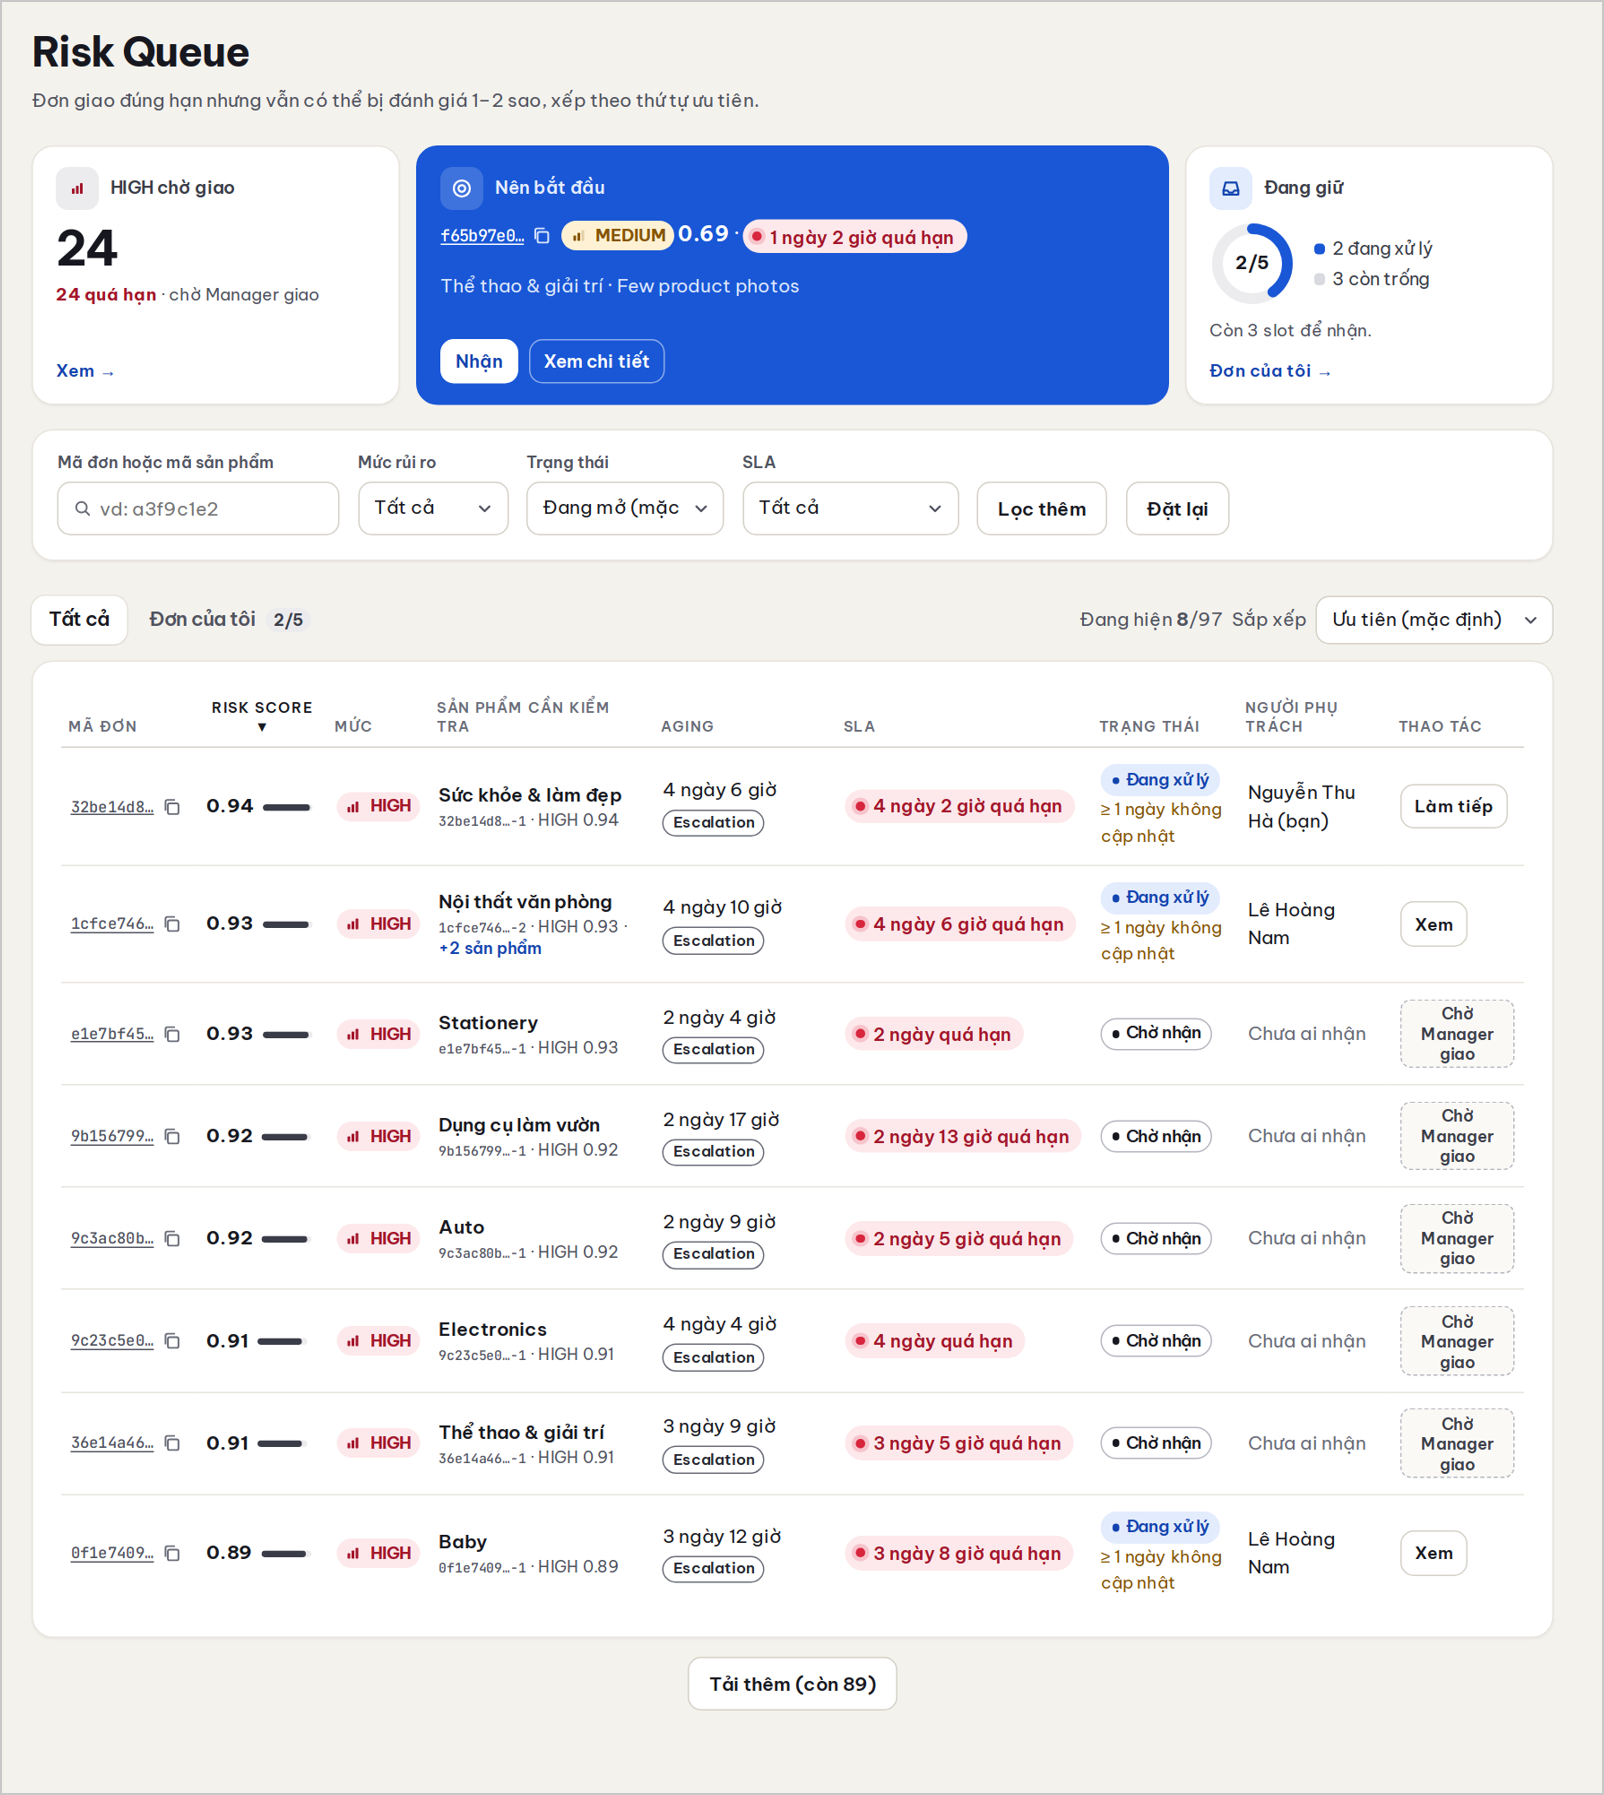
\includegraphics[width=0.85\linewidth]{ui-risk-queue}
  \caption{Hàng đợi rủi ro của nhân viên (dữ liệu demo)}\label{fig:ui-queue}
\end{figure}

\FloatBarrier
% ---------------------------------------------------------------------
\subsection{Diễn giải điểm số ở mức đơn hàng}

Sau khi lựa chọn một đơn từ hàng đợi, người dùng có thể truy cập trang chi tiết để xem thông tin dự báo và các sản phẩm liên quan. Đây là một thành phần quan trọng của hệ thống, bởi điểm rủi ro có thể bị diễn giải sai nếu người dùng chỉ nhìn thấy một con số mà không biết cách nó được tạo ra hoặc giới hạn của nó.

Trang chi tiết đơn (Hình~\ref{fig:ui-detail}) là nơi người dùng xem xét điểm số chi tiết nhất, do đó cũng là nơi có nguy cơ diễn giải sai cao nhất. Khối ``Kết quả model của đơn'' hiển thị bốn thông tin đi cùng điểm số: thanh điểm có vạch ngưỡng của mức trung bình và mức cao, luật tổng hợp, phiên bản mô hình và thời điểm dự báo, phiên bản ngưỡng. Các thông tin này cho phép truy vết mọi con số trên màn hình về đúng lần chấm điểm đã tạo ra nó, cùng nguyên tắc với việc lưu cấu hình và mã commit của từng lần huấn luyện ở mục~\ref{sec:data}.

Bên dưới điểm số là một dòng lưu ý cố định: điểm rủi ro dùng để ưu tiên kiểm tra, không phải kết luận khách không hài lòng. Dòng lưu ý này xuất phát từ hai giới hạn đã nêu ở Chương~\ref{ch:method}. Thứ nhất, nhãn yếu ở mức item: điểm của sản phẩm là rủi ro đơn bị đánh giá thấp khi đơn có chứa sản phẩm đó, không phải bằng chứng sản phẩm gây ra bất mãn. Thứ hai, chỉ số đánh giá đo khả năng xếp hạng, không đo xác suất đúng của từng đơn.

Bảng sản phẩm trong đơn cho thấy điểm của từng item, và khối ``Yếu tố liên quan tới score'' được dành cho giải thích ở mức item. Trong bản demo, một số item có danh sách yếu tố minh họa đi kèm điểm số (Hình~\ref{fig:ui-multi}), số còn lại hiển thị ``chưa có giải thích''. Các yếu tố này là nhãn minh họa của dữ liệu demo, không phải giá trị SHAP; khối này được thiết kế sẵn cho bước giải thích mô hình ở giai đoạn tiếp theo (mục~\ref{sec:demo-limits}). Hai chi tiết thiết kế giúp hạn chế việc diễn giải sai: khi chưa có giải thích, giao diện ghi rõ trạng thái này thay vì để trống, tránh việc người dùng hiểu rằng đơn hàng không có yếu tố rủi ro; khi có giải thích, bên dưới luôn kèm dòng ``các yếu tố này đi kèm điểm cao, không chứng minh nguyên nhân'', nhất quán với quan điểm rằng giá trị SHAP phản ánh cách mô hình sử dụng đặc trưng, không phản ánh tác động nhân quả.

Nhìn chung, trang chi tiết đơn hàng được xây dựng nhằm cung cấp đủ ngữ cảnh để nhân viên sử dụng điểm rủi ro một cách thận trọng, đồng thời hỗ trợ truy vết và mở rộng khả năng giải thích mô hình trong tương lai.

\begin{figure}[!htbp]\centering
  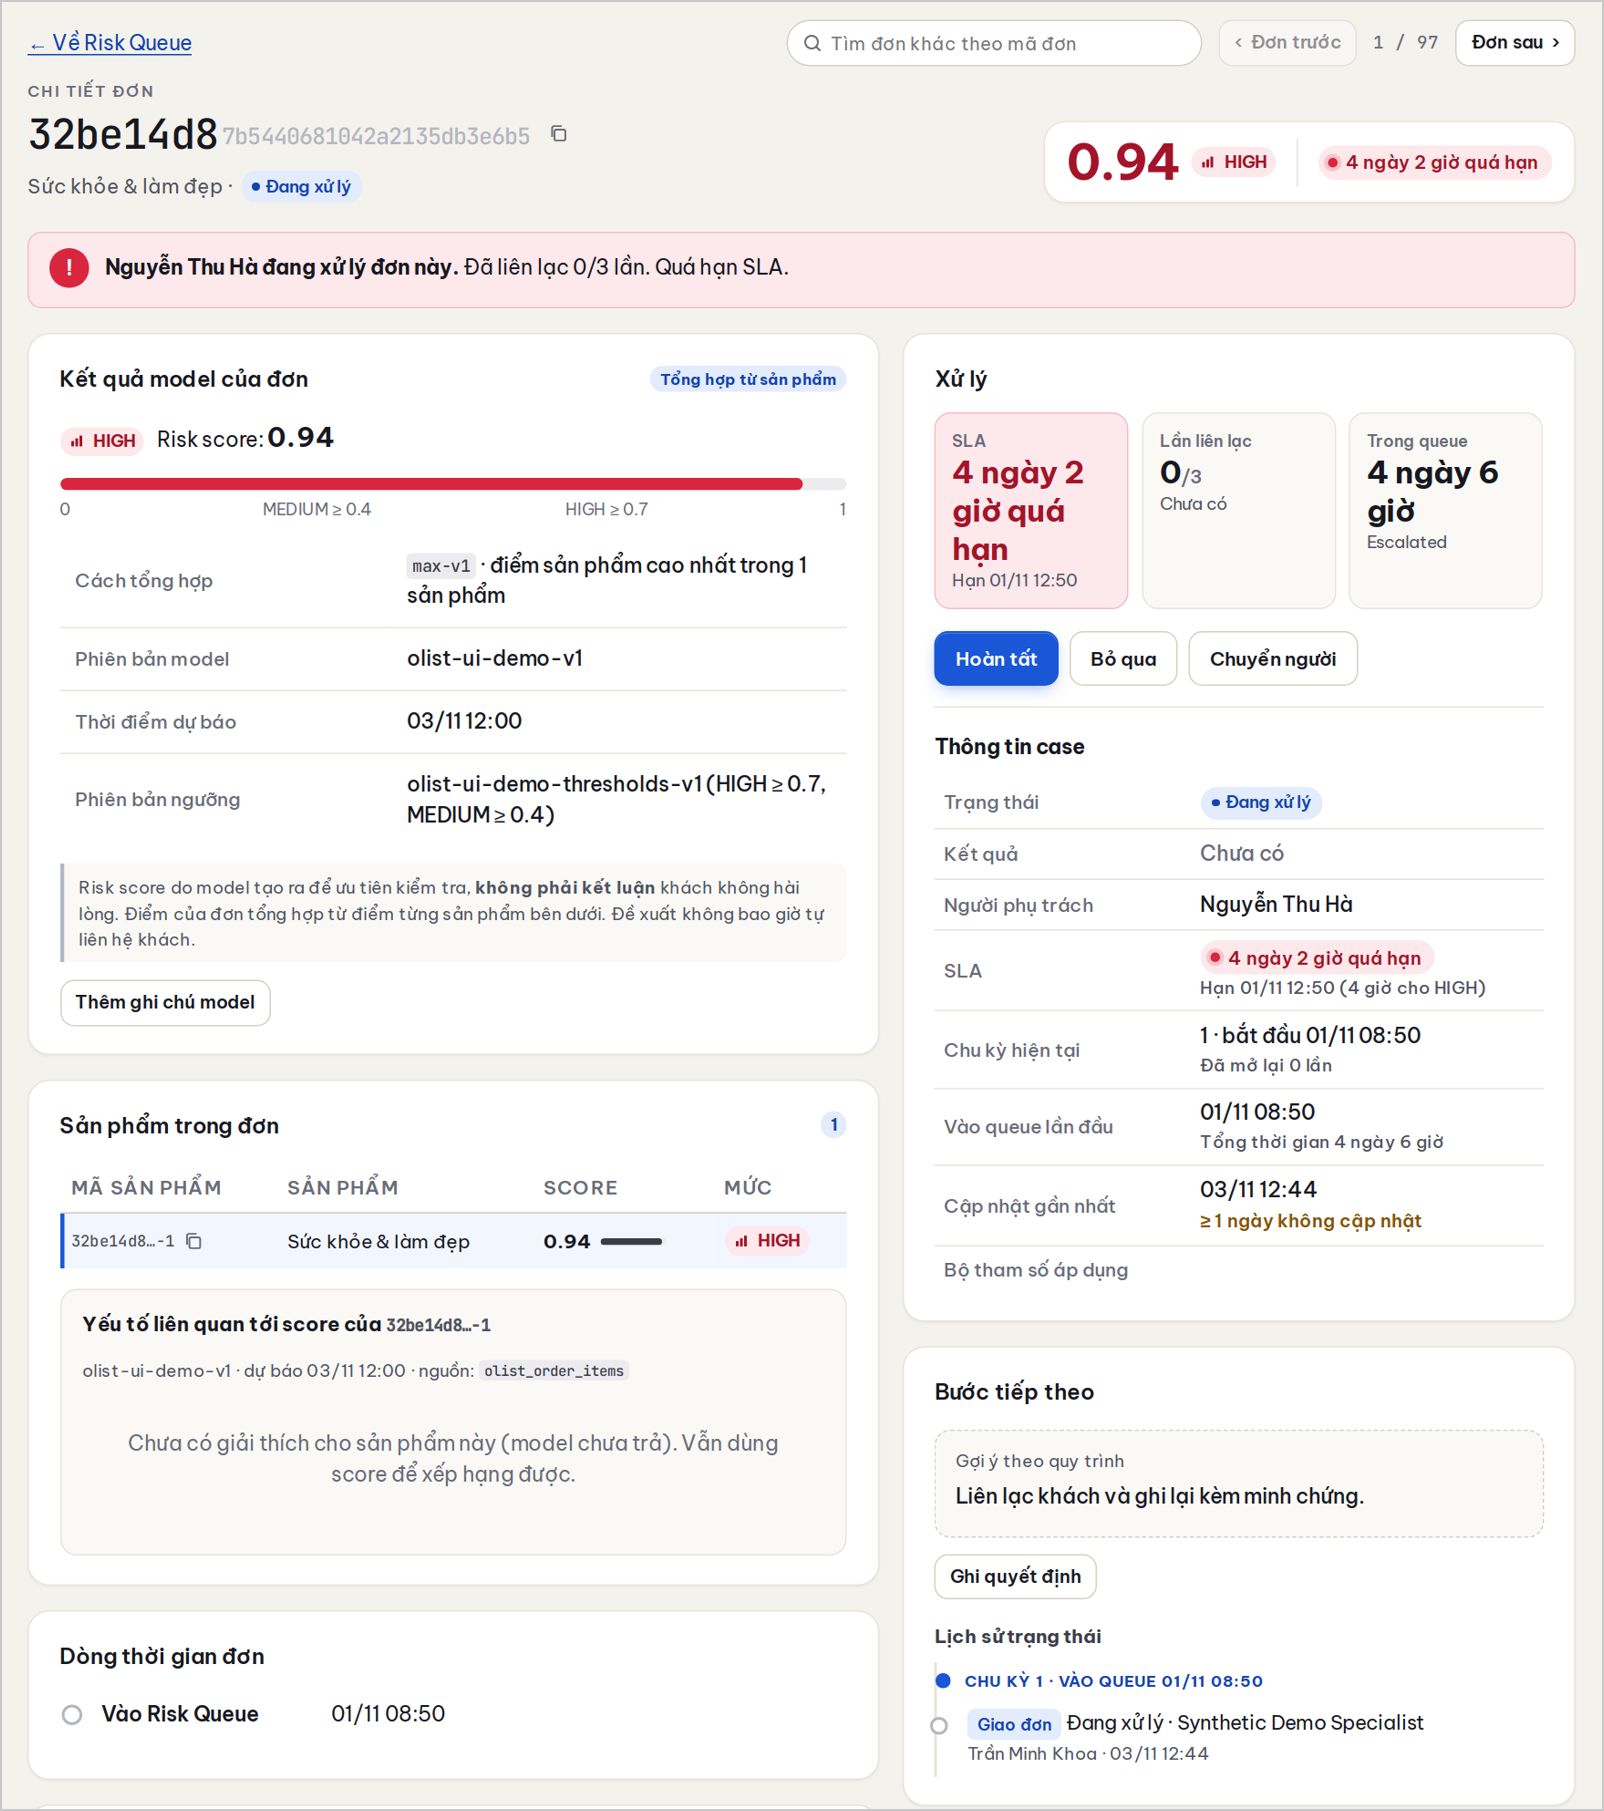
\includegraphics[width=0.85\linewidth]{ui-order-detail}
  \caption{Trang chi tiết đơn (dữ liệu demo)}\label{fig:ui-detail}
\end{figure}

\FloatBarrier
% ---------------------------------------------------------------------
\subsection{Theo dõi phân bố rủi ro}

Bên cạnh hàng đợi dành cho nhân viên, hệ thống còn cung cấp màn tổng quan dành cho quản lý nhằm theo dõi số lượng case và phân bố mức rủi ro.

Màn tổng quan hiển thị số case theo từng mức rủi ro và theo ngày được đưa vào hàng đợi (Hình~\ref{fig:ui-dashboard}). Những thông tin này giúp quản lý theo dõi khối lượng công việc, xác định những nhóm đơn cần phân công và quan sát sự thay đổi của danh sách ưu tiên theo thời gian.

Ngoài vai trò điều phối, các chỉ số tổng quan còn có thể hỗ trợ phát hiện những biến động bất thường trong đầu ra của mô hình.

Chẳng hạn, nếu tỷ lệ đơn được xếp vào mức CAO tăng mạnh giữa hai lần chấm điểm, quản lý có thể nhận biết sự thay đổi này trên giao diện. Trong trường hợp sử dụng mô hình thật, đây có thể là dấu hiệu cần kiểm tra lại phân bố dữ liệu đầu vào, ngưỡng ưu tiên hoặc bước hiệu chỉnh xác suất. Theo Bảng~\ref{tab:split}, tỉ lệ dương dao động từ 10\% đến gần 14\% giữa các giai đoạn, do đó việc theo dõi phân bố theo thời gian là cần thiết khi mô hình được sử dụng lâu dài.

\begin{figure}[!htbp]\centering
  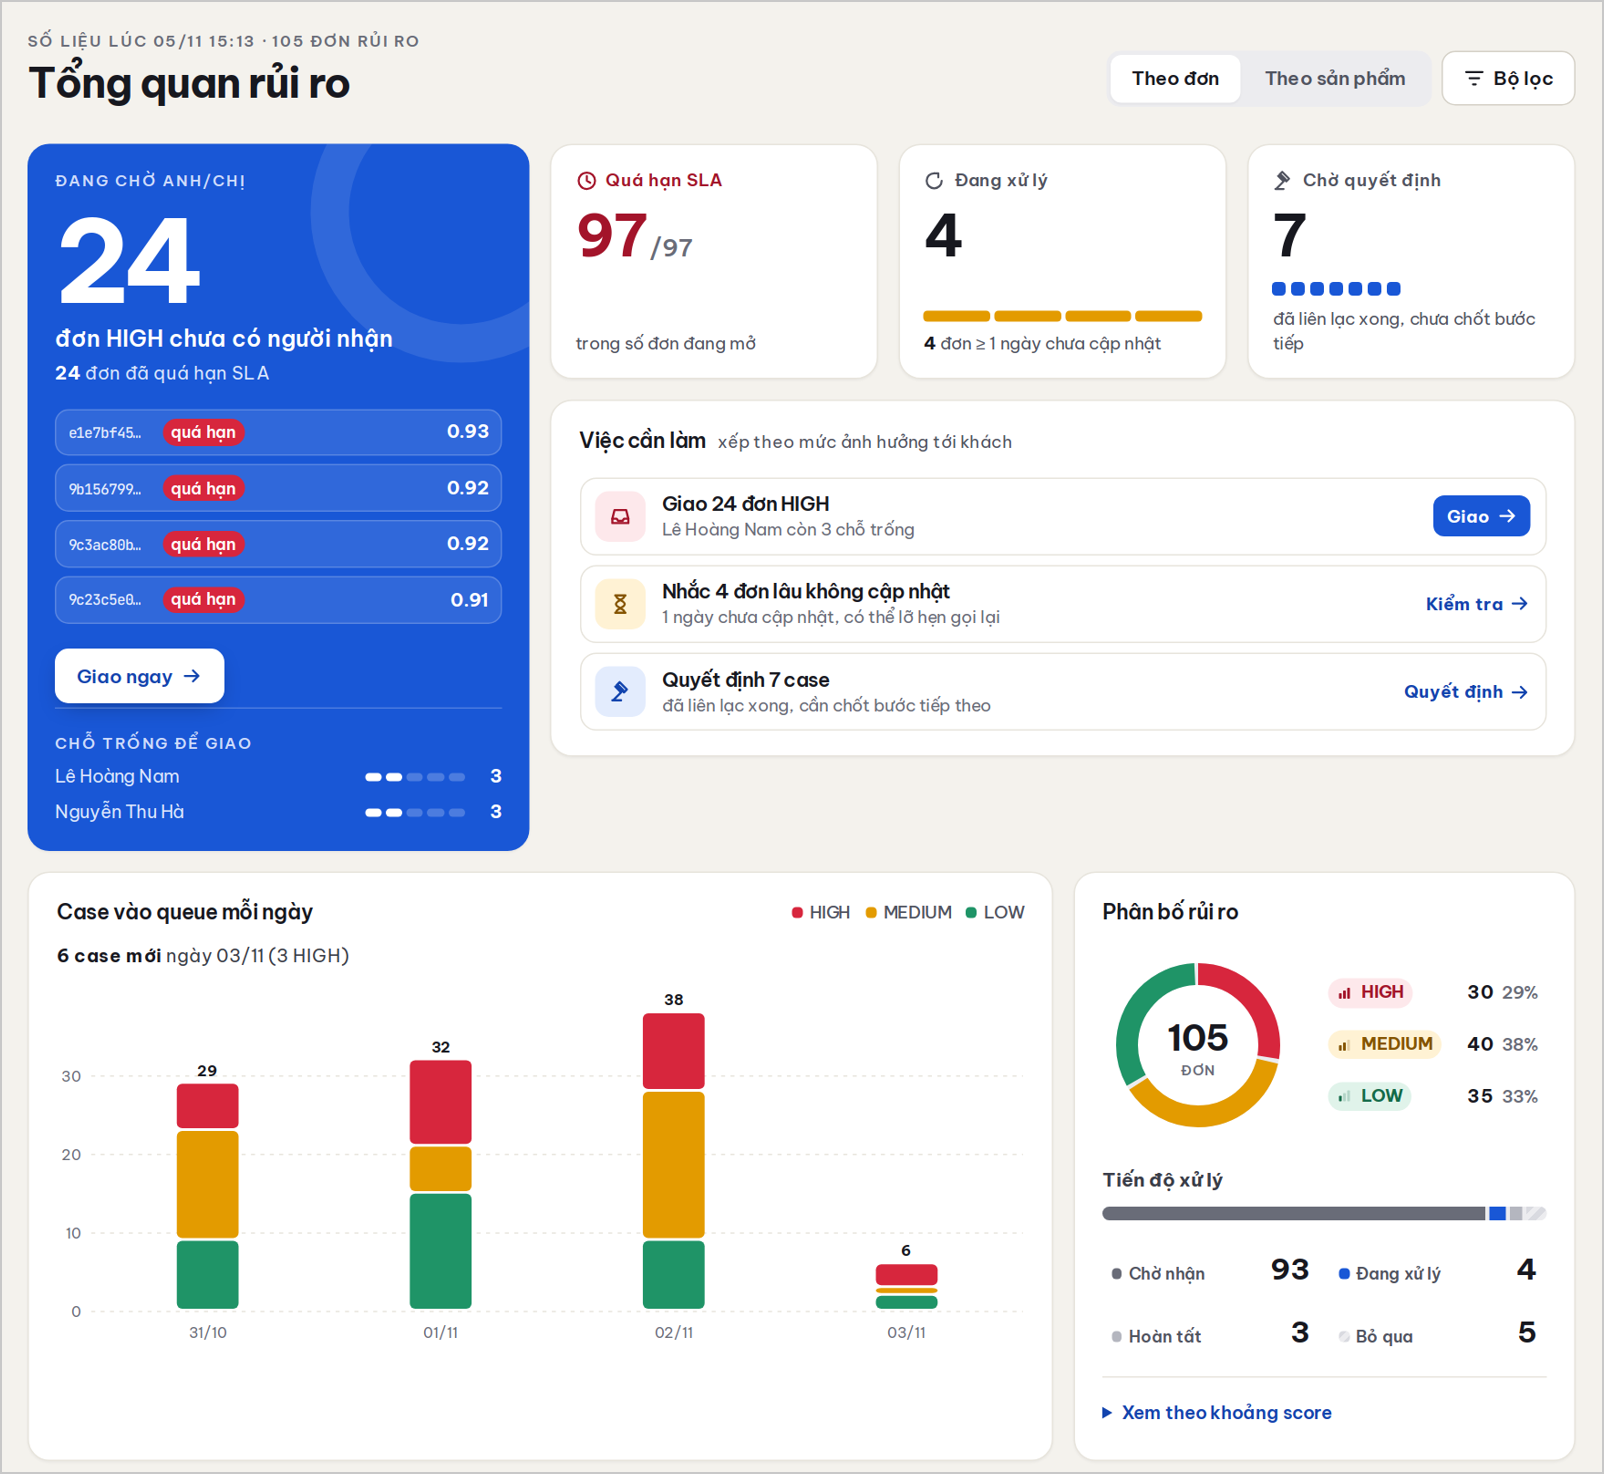
\includegraphics[width=\linewidth]{ui-dashboard}
  \caption{Màn tổng quan rủi ro của quản lý (dữ liệu demo)}\label{fig:ui-dashboard}
\end{figure}

Khối ``Phân bố rủi ro'' trong Hình~\ref{fig:ui-dashboard} cũng minh họa giới hạn quan trọng nhất của bản demo: với ngưỡng cố định 0,7 và 0,4, mức HIGH chiếm 29\% số case (30 trên 105 đơn), trong khi chính sách ở mục~\ref{sec:models} chỉ dành mức này cho 5\% đơn có điểm cao nhất. Nội dung này được phân tích tại mục~\ref{sec:demo-threshold} và Chương~\ref{ch:discussion}.

Bên dưới khối này, phần ``Xem theo khoảng score'' (Hình~\ref{fig:ui-bands}) chia các đơn theo năm khoảng điểm. Với dữ liệu demo, số đơn phân bố tương đối đều giữa các khoảng: lần lượt 15, 20, 26, 26 và 18 đơn từ khoảng thấp nhất đến cao nhất, với điểm trung bình khoảng 0,52. Nếu đây là xác suất đã hiệu chỉnh, kết quả này hàm ý khoảng một nửa số đơn giao đúng hạn sẽ bị đánh giá thấp, trong khi tỉ lệ thực tế chỉ khoảng 10\%. Với một mô hình được hiệu chỉnh tốt, trung bình xác suất dự đoán phải xấp xỉ tỉ lệ dương, và phần lớn đơn hàng sẽ tập trung ở các khoảng điểm thấp. Do đó, bảng khoảng điểm có thể được sử dụng như một phép kiểm tra nhanh ở phía vận hành: nếu điểm trung bình lệch xa tỉ lệ đơn bị đánh giá thấp quan sát được, hoặc hình dạng phân bố thay đổi mạnh giữa hai lần chấm điểm, cần rà soát lại bước hiệu chỉnh hoặc dữ liệu đầu vào.

\begin{figure}[!htbp]\centering
  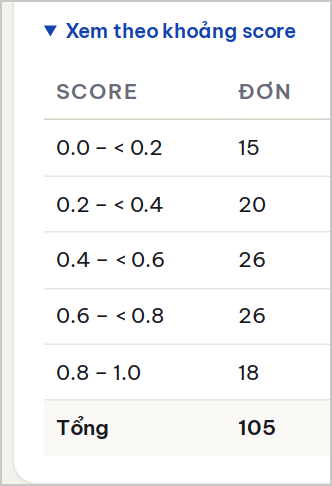
\includegraphics[width=0.3\linewidth]{ui-score-bands}
  \caption{Số đơn theo khoảng điểm (dữ liệu demo)}\label{fig:ui-bands}
\end{figure}

Màn tổng quan còn có chế độ ``Theo sản phẩm'', trong đó các khối thống kê được tính theo đơn vị item: 105 đơn trong bản demo gồm 114 sản phẩm. Hình~\ref{fig:ui-product} trích phần danh sách sản phẩm có điểm cao nhất của chế độ này; mỗi dòng là một item, mang mã đơn kèm số thứ tự sản phẩm trong đơn, danh mục, trạng thái của case và yếu tố minh họa nếu có. Hai chế độ tương ứng với hai đơn vị đã tách ở mục~\ref{sec:pipeline}: mô hình học và chấm điểm ở mức item, còn nhân viên xử lý ở mức đơn. Việc trình bày song song hai góc nhìn giúp người dùng phân biệt số sản phẩm rủi ro với số đơn cần liên hệ.

\begin{figure}[!htbp]\centering
  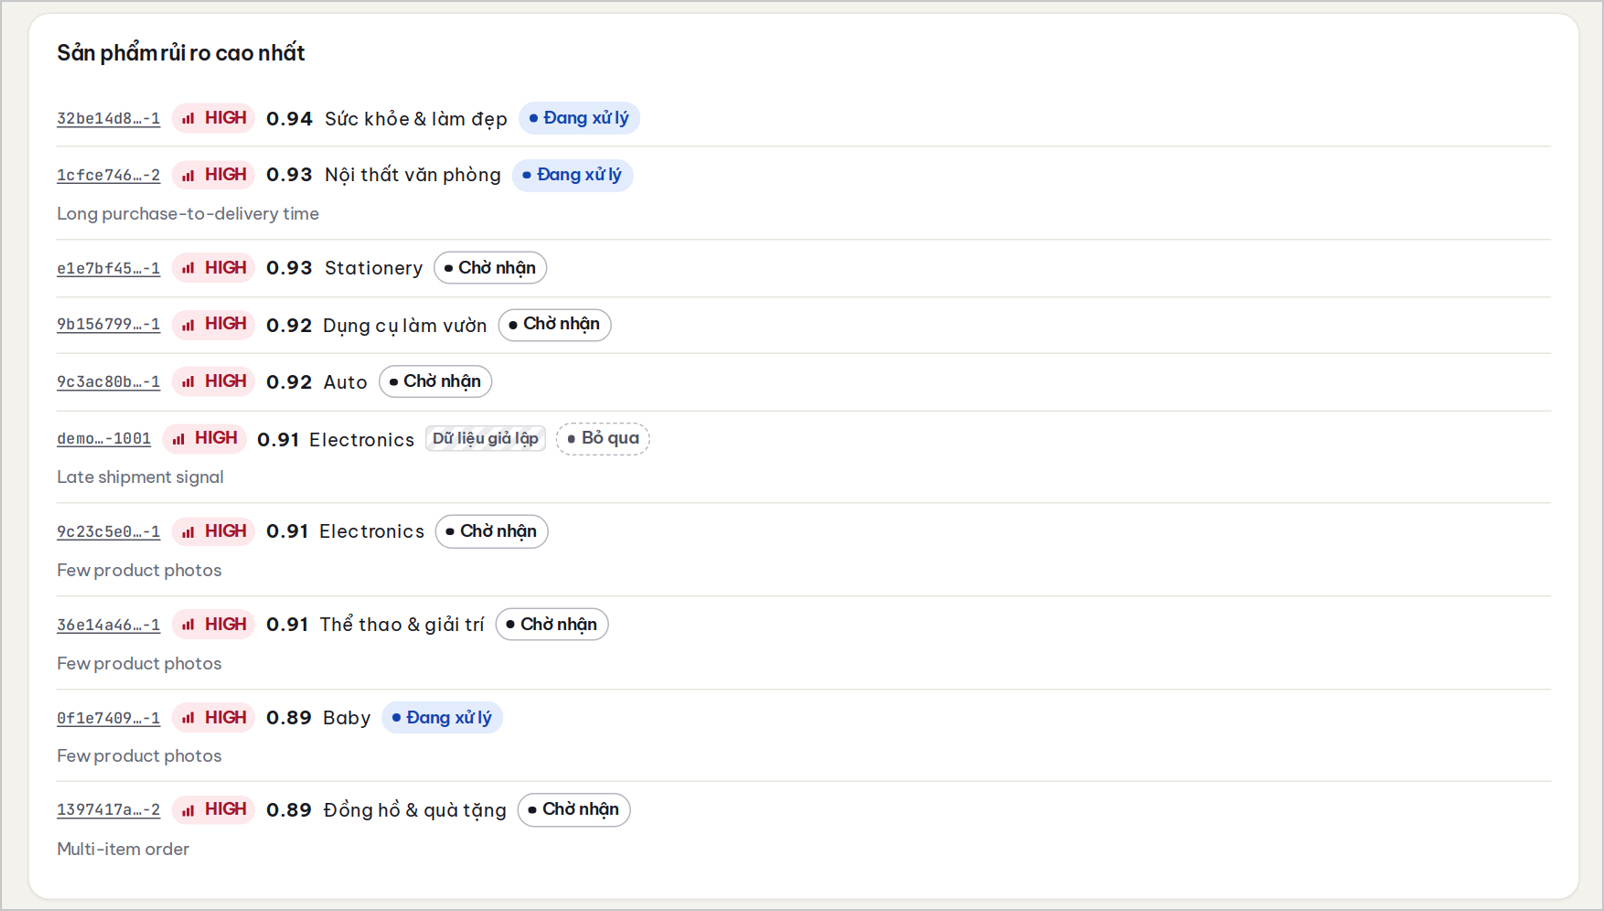
\includegraphics[width=\linewidth]{ui-product-view}
  \caption{Chế độ xem theo sản phẩm (dữ liệu demo)}\label{fig:ui-product}
\end{figure}

\FloatBarrier
% ---------------------------------------------------------------------
\subsection{Dữ liệu vận hành phục vụ đánh giá mô hình}

Như đã nêu ở mục~\ref{sec:eval}, các chỉ số hiện tại chỉ đánh giá khả năng dự báo của mô hình, chưa cho biết việc chủ động liên hệ với khách hàng có thực sự cải thiện kết quả hay không.

Để có thể đánh giá vấn đề này trong tương lai, ứng dụng được thiết kế nhằm ghi nhận những thông tin phát sinh trong quá trình xử lý case, thay vì chỉ hiển thị điểm dự báo.

Quá trình lưu trữ dữ liệu vận hành tuân theo ba nguyên tắc chính.

\begin{enumerate}
  \item \textbf{Điểm số chỉ đọc.} Không có thao tác nào sửa điểm hay mức rủi ro. Quản lý có thể thêm ghi chú về mô hình cho một đơn, nhưng ghi chú được lưu riêng. Nhờ đó, điểm gốc có thể được so sánh với kết quả thực tế mà không chịu ảnh hưởng của điều chỉnh thủ công.
  \item \textbf{Kết quả xử lý có cấu trúc.} Khi đóng case, nhân viên phải chọn một kết quả trong danh mục cố định (có vấn đề, không có vấn đề, trùng case) hoặc một lý do bỏ qua (không liên lạc được, khách từ chối, \ldots). Mỗi lần liên lạc được ghi lại với cách liên lạc và kết quả. Kết quả ``có vấn đề'' và ``không có vấn đề'' là một nguồn nhãn độc lập với đánh giá sao, có thể dùng để đo precision của nhóm HIGH trong vận hành thật.
  \item \textbf{Lịch sử chỉ thêm, không sửa.} Mọi thao tác đều được ghi lại với thời điểm và người thực hiện, cho phép tái dựng việc đơn nào đã được liên hệ, vào thời điểm nào và sau bao lâu kể từ khi có điểm, phục vụ đối chiếu với nhãn quan sát được về sau.
\end{enumerate}

Mỗi lần liên hệ được ghi qua màn hình liên lạc khách (Hình~\ref{fig:ui-contact}) với thời điểm, phương thức, kết quả và ngày hẹn liên hệ tiếp. Đây là dữ liệu về can thiệp, loại dữ liệu mà bộ Olist không có. Khi sử dụng cho mục đích đánh giá, cần phân biệt hai trường hợp: nếu sau số lần liên hệ tối đa vẫn không liên lạc được với khách hàng, case tự động chuyển sang trạng thái bỏ qua với lý do ``không liên lạc được'', nghĩa là can thiệp chưa diễn ra; trường hợp này khác với trường hợp can thiệp đã diễn ra nhưng khách hàng vẫn đánh giá thấp. Nếu gộp hai nhóm, hiệu quả can thiệp sẽ bị ước lượng thấp hơn thực tế.

\begin{figure}[!htbp]\centering
  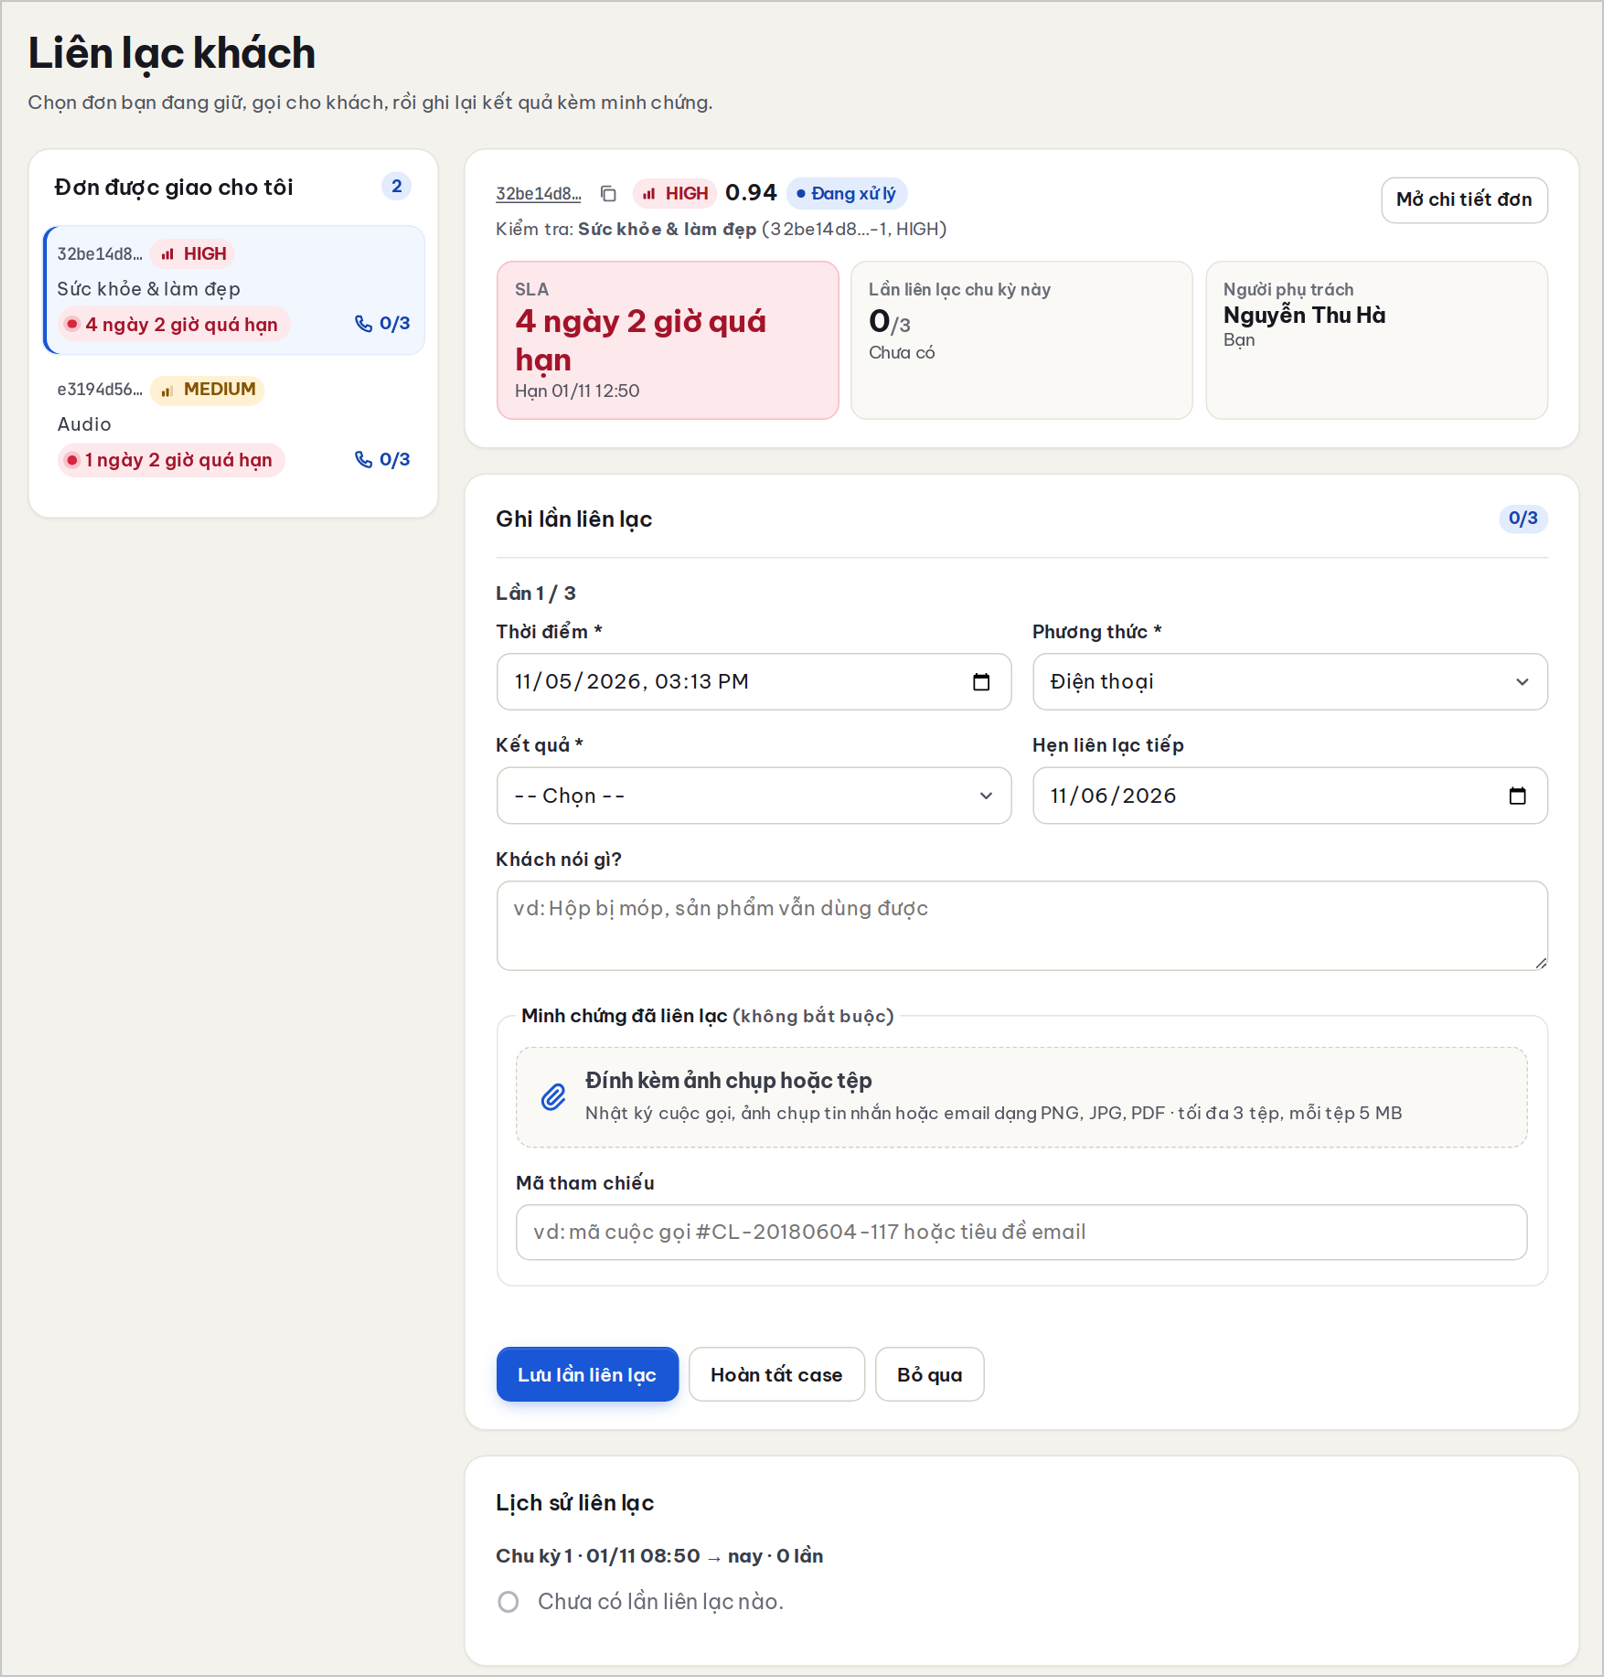
\includegraphics[width=0.8\linewidth]{ui-contact-attempt}
  \caption{Biểu mẫu ghi lần liên lạc (dữ liệu demo)}\label{fig:ui-contact}
\end{figure}

Hình~\ref{fig:ui-closed} là một case đã đóng: điểm 0,68 ở mức trung bình được hiển thị cùng kết quả xử lý ``có vấn đề'', lịch sử trạng thái và quyết định tiếp theo của quản lý. Mỗi case đóng như vậy là một cặp (điểm dự báo, kết quả quan sát) gắn với đúng phiên bản mô hình đã sinh ra điểm. Hình~\ref{fig:feedback-loop} tóm tắt cách các cặp dữ liệu này được sử dụng để đánh giá và cải tiến mô hình; đường nét đứt trong hình là bước đề tài chưa thực hiện.

\begin{figure}[!htbp]\centering
  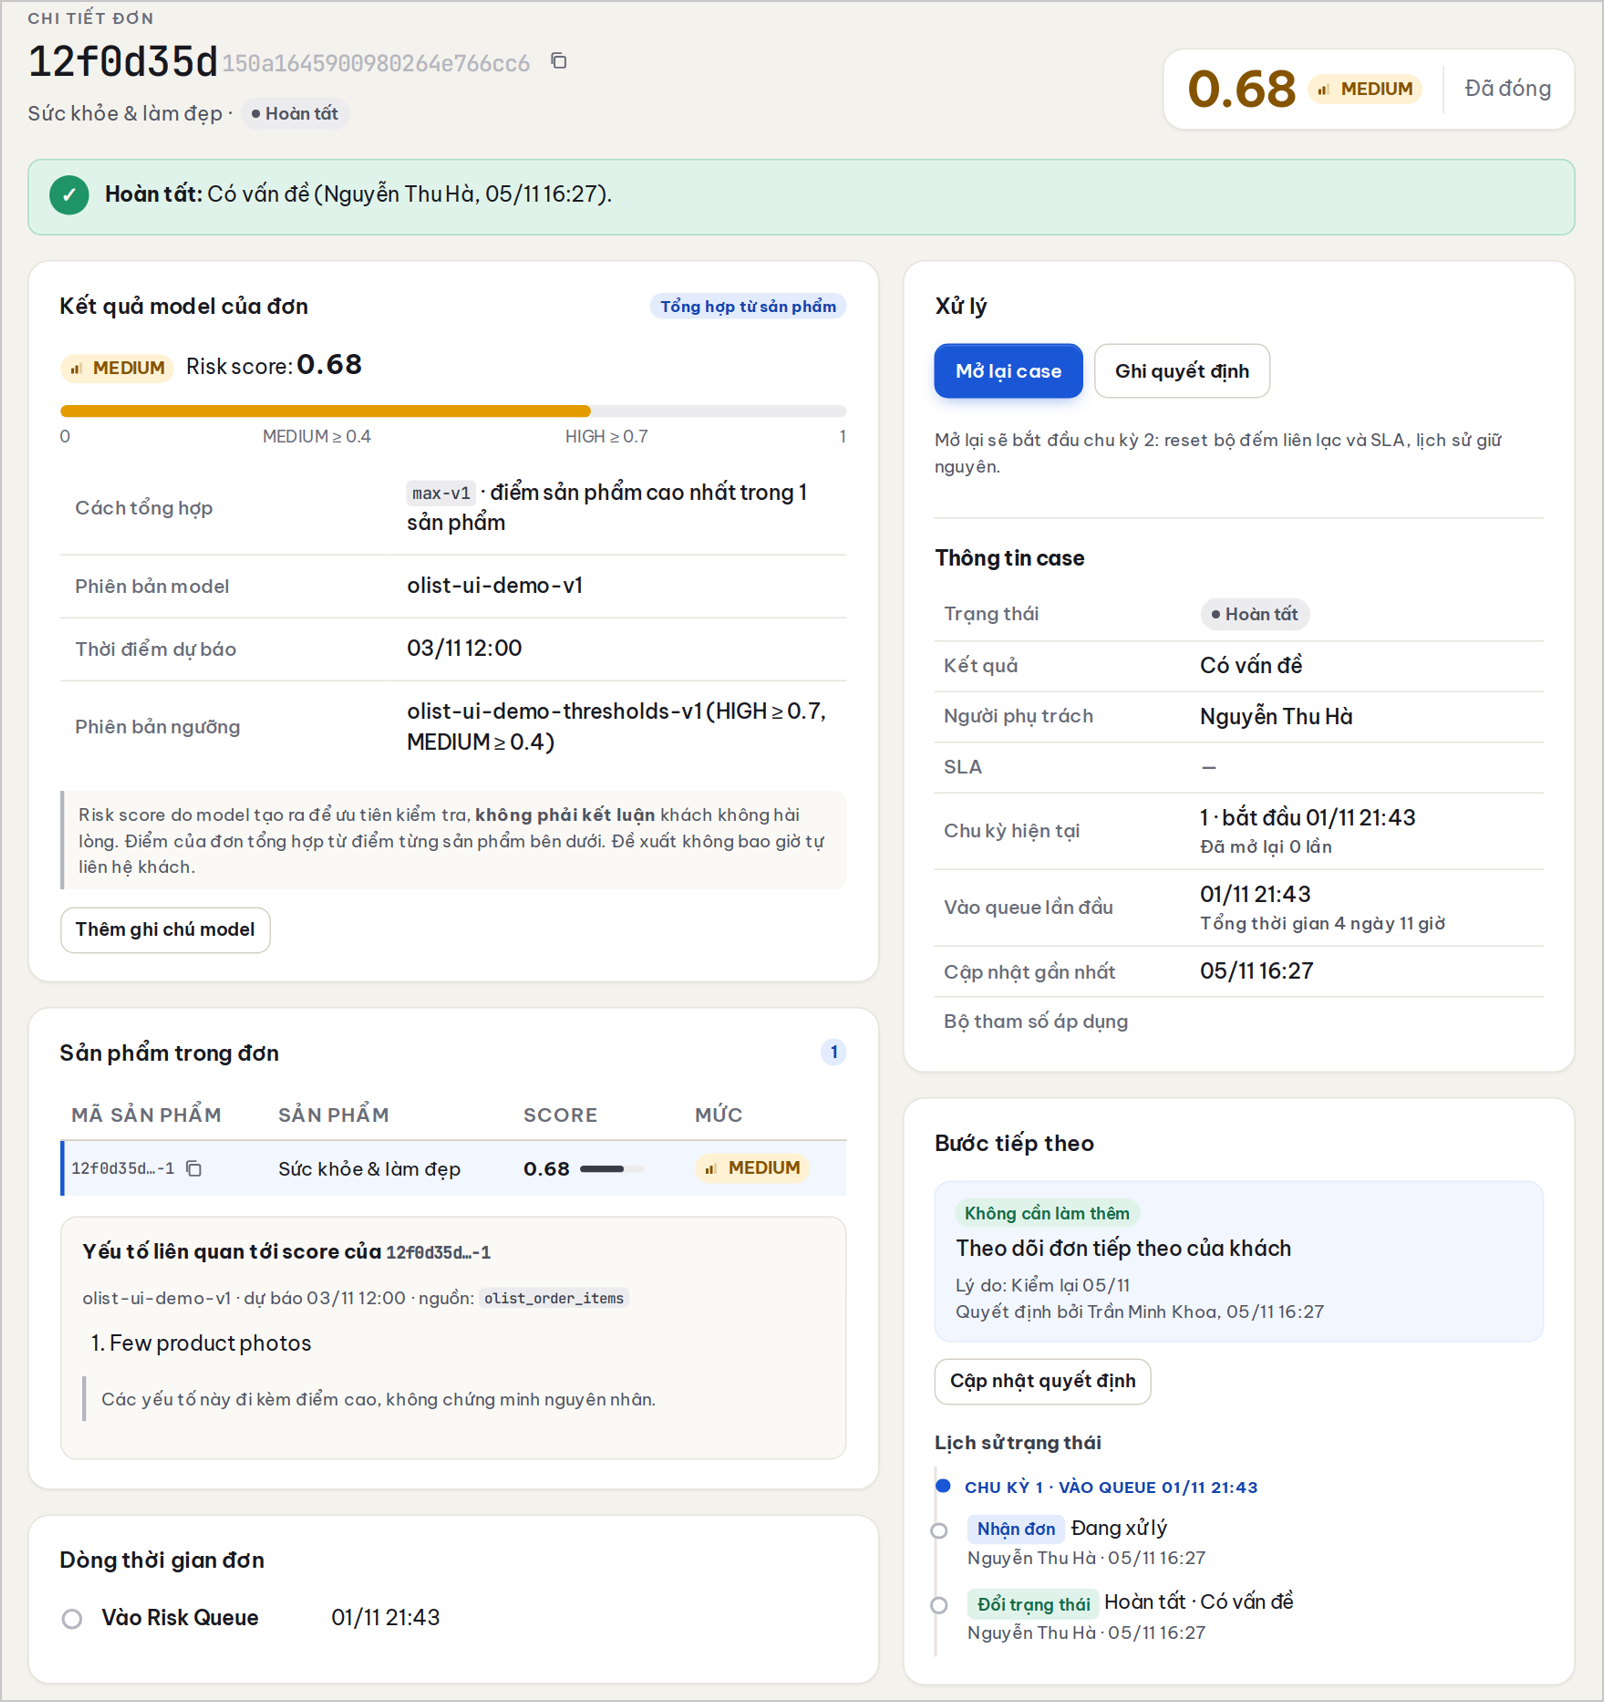
\includegraphics[width=0.8\linewidth]{ui-closed-case}
  \caption{Case đã đóng (dữ liệu demo)}\label{fig:ui-closed}
\end{figure}

\begin{figure}[!htbp]\centering
\begin{tikzpicture}[font=\footnotesize, >={Latex}, node distance=0.55cm and 0.9cm,
  box/.style={draw,rounded corners,fill=#1,minimum width=3.4cm,minimum height=0.9cm,align=center}, box/.default=gray!10]
  \node[box=blue!15] (snap) {Snapshot dự đoán\\điểm, mức, phiên bản};
  \node[box=orange!20,right=of snap] (case) {Case trong\\hàng đợi ưu tiên};
  \node[box=teal!20,right=of case] (contact) {Liên hệ khách\\(các lần liên lạc)};
  \node[box=green!20,below=of contact] (outcome) {Kết quả xử lý\\có / không có vấn đề};
  \node[box=yellow!30,left=of outcome] (eval) {Cặp (điểm, kết quả)\\precision nhóm HIGH};
  \node[box=violet!20,left=of eval] (retrain) {Hiệu chỉnh, chọn ngưỡng\\hoặc huấn luyện lại};
  \node[box=red!15,below=of eval] (review) {Đánh giá sao của khách\\(nhãn $y$ ở Chương~3)};
  \draw[->] (snap) -- (case); \draw[->] (case) -- (contact); \draw[->] (contact) -- (outcome);
  \draw[->] (outcome) -- (eval); \draw[->] (review) -- (eval); \draw[->] (eval) -- (retrain);
  \draw[->,dashed] (retrain) -- node[right,font=\scriptsize]{phiên bản mới} (snap);
\end{tikzpicture}
\caption{Vòng phản hồi giữa ứng dụng và luồng học máy}\label{fig:feedback-loop}
\end{figure}

Trong tương lai, những thông tin này có thể hỗ trợ hiệu chỉnh xác suất, điều chỉnh ngưỡng hoặc huấn luyện lại mô hình khi có thêm dữ liệu phù hợp.

Đồng thời, hệ thống cũng tạo tiền đề cho việc thực hiện thử nghiệm có đối chứng. Chẳng hạn, nếu một phần đơn thuộc nhóm rủi ro cao được chọn ngẫu nhiên để không liên hệ, nhóm có thể so sánh kết quả giữa nhóm được liên hệ và nhóm đối chứng nhằm ước lượng tác động của hoạt động chăm sóc khách hàng.

Tuy nhiên, thử nghiệm này chưa được thực hiện trong phạm vi đề tài. Vì vậy, hệ thống hiện mới cung cấp cơ chế thu thập dữ liệu cần thiết, chưa có bằng chứng trực tiếp về hiệu quả của hoạt động can thiệp.

\FloatBarrier
% ---------------------------------------------------------------------
\subsection{Minh họa luật tổng hợp max-v1}\label{sec:demo-maxv1}

Như đã trình bày ở mục 3.1.1, mô hình tạo điểm dự báo ở cấp sản phẩm, trong khi hoạt động chăm sóc khách hàng được thực hiện ở cấp đơn hàng. Vì vậy, cần có một quy tắc tổng hợp để chuyển các điểm sản phẩm thành một điểm đại diện cho toàn bộ đơn.

Luật max-v1 quyết định thứ tự của đơn hàng trong hàng đợi, vì vậy cần làm rõ điểm khác biệt giữa luật này và cách lấy trung bình. Bảng~\ref{tab:demo-maxv1} sử dụng ba đơn với điểm item giả định, nhằm minh họa cơ chế tổng hợp; mức rủi ro được gán theo ngưỡng của lần chạy rừng ngẫu nhiên đã nêu ở mục~\ref{sec:demo-limits} (mức cao từ 0,286, mức trung bình từ 0,112).

\begin{table}[htbp]\centering\small
\caption{Điểm đơn theo luật max-v1 và theo trung bình (điểm item giả định)}\label{tab:demo-maxv1}
\begin{tabular}{lp{3.4cm}cccc}
\toprule
Đơn & Điểm các item & max-v1 & Mức & Trung bình & Mức \\
\midrule
A & 0,08; 0,12; 0,41       & 0,41 & \textsc{Cao}        & 0,20 & \textsc{Trung bình} \\
B & 0,30                   & 0,30 & \textsc{Cao}        & 0,30 & \textsc{Cao} \\
C & 0,15; 0,16; 0,18; 0,20 & 0,20 & \textsc{Trung bình} & 0,17 & \textsc{Trung bình} \\
\bottomrule
\end{tabular}
\end{table}

Hình~\ref{fig:ui-multi} là một đơn ba sản phẩm trong bản demo: các item có điểm 0,93, 0,79 và 0,43, điểm của đơn là 0,93 theo max-v1, trong khi trung bình chỉ là 0,72. Giao diện đánh dấu item quyết định điểm của đơn ở dòng đầu bảng sản phẩm, giúp người dùng xác định nguồn gốc điểm số của đơn.

\begin{figure}[!htbp]\centering
  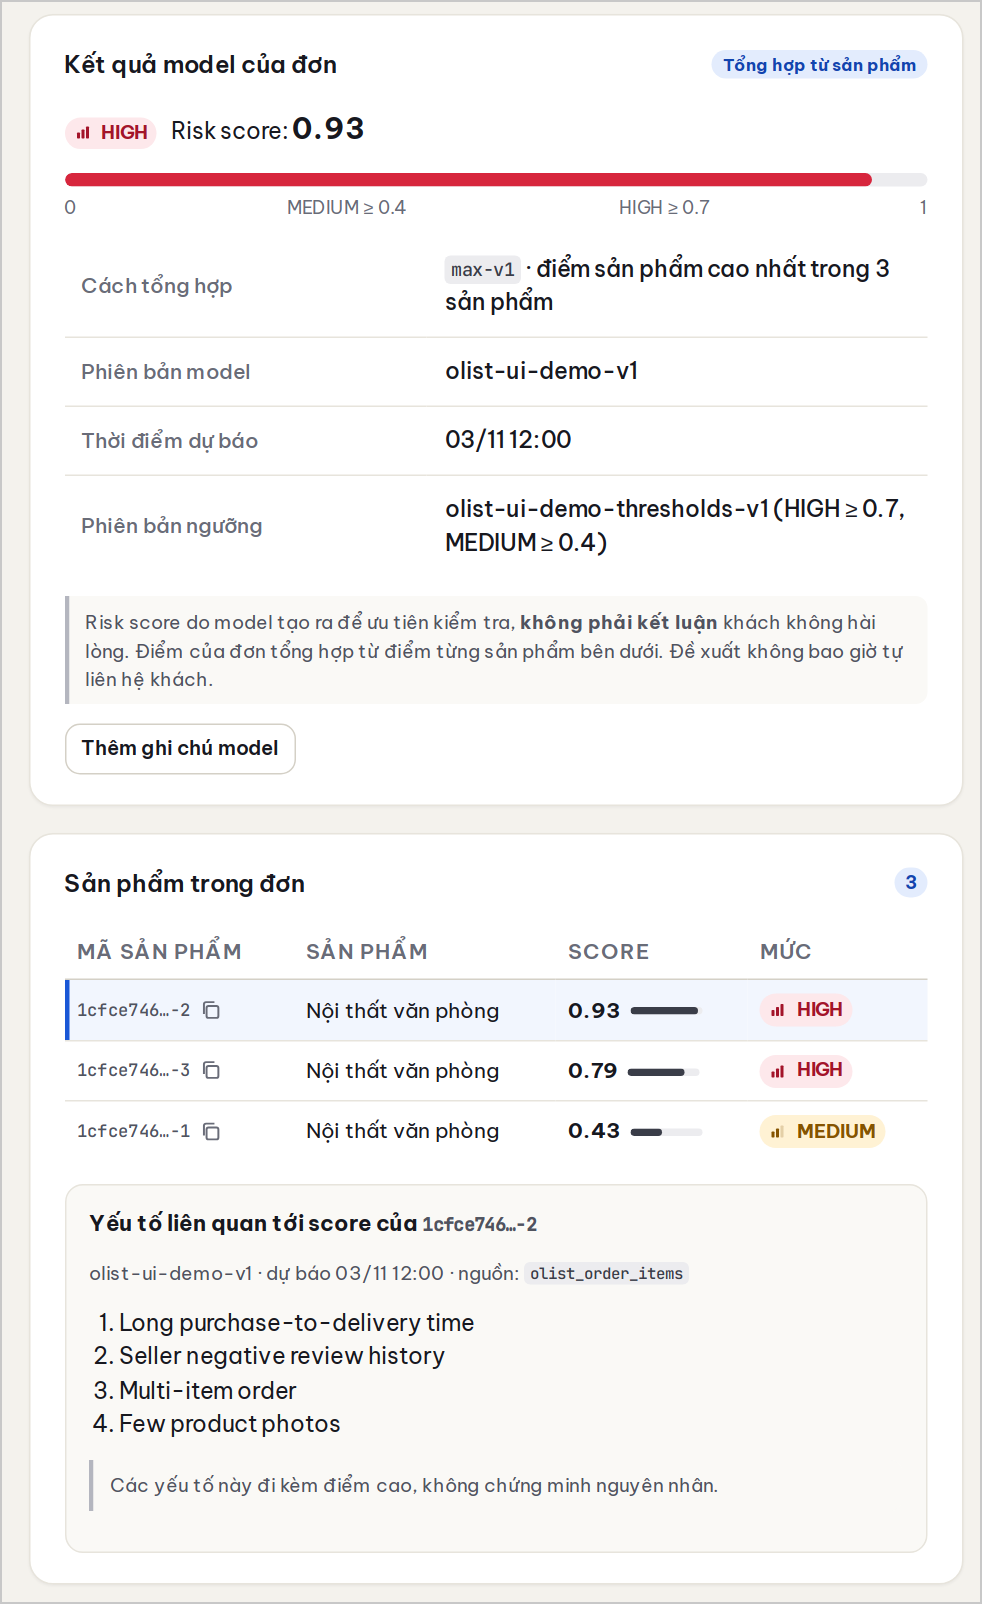
\includegraphics[width=0.62\linewidth]{ui-multi-item}
  \caption{Đơn ba sản phẩm theo luật max-v1 (dữ liệu demo)}\label{fig:ui-multi}
\end{figure}

Theo max-v1, ba đơn giả định trong Bảng~\ref{tab:demo-maxv1} có thứ tự ưu tiên là A, B, C; theo trung bình, thứ tự là B, A, C. Khác biệt nằm ở đơn A: khi lấy trung bình, điểm 0,41 của một sản phẩm bị hai sản phẩm có điểm thấp kéo xuống còn 0,20, và đơn không còn thuộc mức cao. Đây là tình huống ``mắt xích yếu nhất'' mà luật max-v1 được thiết kế để phát hiện (mục~\ref{sec:pipeline}). 

Ở đơn C trong Bảng 4.9, cả bốn sản phẩm đều có điểm tương đối gần nhau và không có sản phẩm nào nổi bật như trường hợp A. Dù vậy, điểm tổng hợp của đơn vẫn được lấy bằng giá trị lớn nhất là 0,20. Khi số lượng sản phẩm trong đơn tăng, khả năng xuất hiện một điểm cao cũng tăng theo. Vì vậy, max-v1 có thể tạo xu hướng ưu tiên những đơn nhiều sản phẩm, ngay cả khi từng sản phẩm riêng lẻ không có mức rủi ro cao hơn. Để hỗ trợ người dùng phân biệt những tình huống này, giao diện hiển thị điểm của từng sản phẩm và đánh dấu sản phẩm có điểm cao nhất. Nhờ đó, nhân viên có thể nhận biết liệu điểm tổng hợp xuất phát từ một sản phẩm có rủi ro nổi bật hay từ nhiều sản phẩm có điểm tương đối tương đồng.

Nhìn chung, max-v1 phù hợp với giả định rằng một sản phẩm có vấn đề có thể ảnh hưởng đến đánh giá chung của đơn hàng. Tuy nhiên, tác động của quy tắc này đối với những đơn nhiều sản phẩm vẫn cần được kiểm chứng thêm bằng dữ liệu dự báo thực tế ở cấp đơn.

\FloatBarrier
% ---------------------------------------------------------------------
\subsection{Tác động của ngưỡng lên danh sách ưu tiên}\label{sec:demo-threshold}

Bên cạnh quy tắc tổng hợp, cách xác định ngưỡng rủi ro cũng ảnh hưởng trực tiếp đến số lượng đơn được đưa vào từng mức ưu tiên.

Bảng~\ref{tab:demo-threshold} so sánh tỉ lệ các mức rủi ro trong bản demo (ngưỡng cố định 0,7 và 0,4, đếm trên 105 case ở Hình~\ref{fig:ui-dashboard}) với tỉ lệ mà chính sách ngưỡng ở mục~\ref{sec:models} tạo ra. Vì điểm của bản demo không phải đầu ra của mô hình, bảng không so sánh hai bộ điểm mà so sánh hai cách đặt ngưỡng.

\begin{table}[htbp]\centering\small
\caption{Tỉ lệ các mức rủi ro: ngưỡng cố định của bản demo và chính sách theo phần trăm}\label{tab:demo-threshold}
\begin{tabular}{lcccc}
\toprule
Cách đặt ngưỡng & Ngưỡng cao / trung bình & \textsc{Cao} & \textsc{Trung bình} & \textsc{Thấp} \\
\midrule
Cố định (bản demo, 105 case)        & 0,7 / 0,4         & 29\% (30) & 38\% (40) & 33\% (35) \\
Theo phần trăm (chính sách)         & $\approx$0,286 / $\approx$0,112 & 5\%  & 15\% & 80\% \\
\bottomrule
\end{tabular}
\end{table}

Kết quả cho thấy việc sử dụng ngưỡng cố định trong bản demo khiến gần một phần ba số case được xếp vào mức CAO. Trong khi đó, chính sách theo phần trăm chỉ dành mức này cho 5% số đơn có điểm cao nhất.

Sự khác biệt này có ý nghĩa trực tiếp đối với hoạt động chăm sóc khách hàng. Nếu quá nhiều đơn được gắn mức ưu tiên cao, bộ phận quản lý có thể gặp khó khăn trong việc xác định những trường hợp cần xử lý trước.

Ngược lại, ngưỡng theo tỷ lệ phần trăm giúp giới hạn số đơn được xếp mức CAO theo một tỷ lệ đã xác định. Khi được lựa chọn phù hợp với nguồn lực, phương pháp này có thể hỗ trợ phân bổ công việc hiệu quả hơn.

Một vấn đề khác cũng cần được xem xét khi chuyển từ điểm minh họa sang điểm dự báo của mô hình thật.

Trong một lần chạy Random Forest trước đó, ngưỡng mức CAO được xác định khoảng 0,286, thấp hơn đáng kể so với ngưỡng cố định 0,7 của bản demo. Nếu tiếp tục sử dụng ngưỡng 0,7 với phân bố điểm của mô hình thật, số đơn thuộc mức CAO có thể thấp hơn nhiều so với mục tiêu 5%, khiến một phần năng lực xử lý không được sử dụng.

Vì vậy, ngưỡng ưu tiên cần được xác định dựa trên phân bố điểm của mô hình và giới hạn nguồn lực vận hành, thay vì lựa chọn một giá trị cố định không có cơ sở từ dữ liệu.

Đồng thời, mỗi lần thay đổi tham số trong hệ thống đều tạo ra một phiên bản mới, kèm thời điểm có hiệu lực và lý do điều chỉnh. Cơ chế này giúp truy vết điều kiện vận hành đã được áp dụng cho từng case, phục vụ việc đánh giá về sau.

Nhìn chung, kết quả minh họa cho thấy cách đặt ngưỡng có thể làm thay đổi đáng kể quy mô hàng đợi ưu tiên. Vì vậy, ngưỡng cần được xem là một thành phần của chính sách phân bổ nguồn lực, chứ không chỉ là một giá trị dùng để phân loại điểm số.

\begin{figure}[!htbp]\centering
  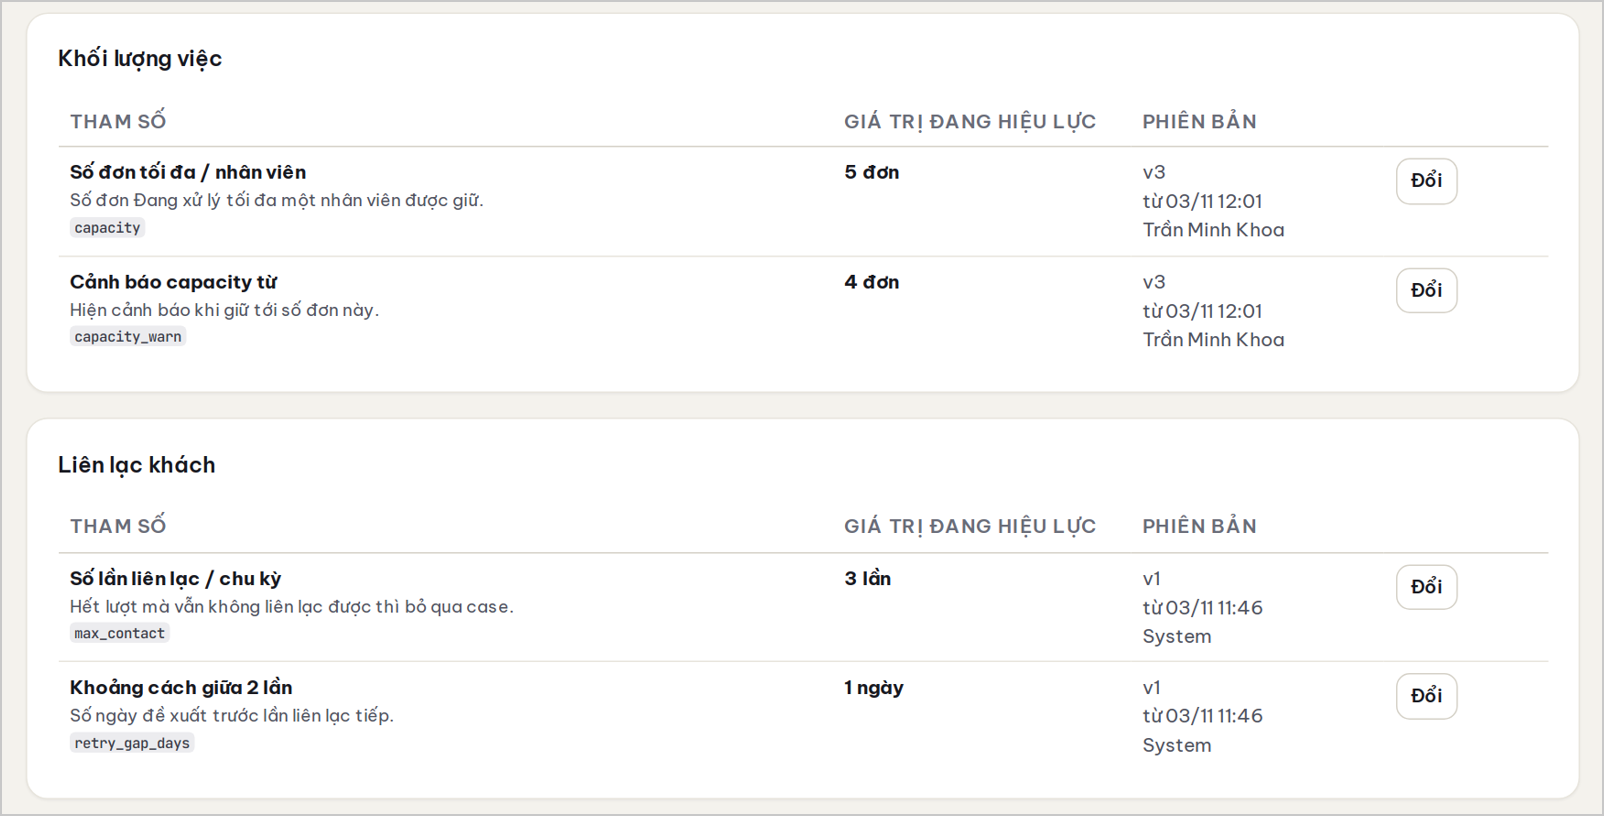
\includegraphics[width=\linewidth]{ui-settings-capacity}
  \caption{Tham số năng lực xử lý (dữ liệu demo)}\label{fig:ui-settings}
\end{figure}

\FloatBarrier
% ---------------------------------------------------------------------
\subsection{Giới hạn của bản demo}\label{sec:demo-limits}

Ứng dụng đã minh họa được quy trình xử lý từ việc tiếp nhận điểm rủi ro đến tạo hàng đợi, phân công nhân viên, ghi nhận liên hệ và đóng case. Tuy nhiên, khả năng vận hành của giao diện chưa đồng nghĩa với việc mô hình học máy đã được triển khai và kiểm chứng trong điều kiện thực tế. Hiện tại, giữa kết quả nghiên cứu và ứng dụng demo vẫn tồn tại ba khoảng cách cần được giải quyết.

\begin{enumerate}
  \item \textbf{Điểm số minh họa thay vì điểm của mô hình.} Trước hết, điểm rủi ro hiển thị trên ứng dụng vẫn là điểm minh họa, không phải kết quả suy luận của mô hình Random Forest được lựa chọn. Lần rà soát toàn luồng ngày 31/10/2026 ghi nhận tệp mô hình nạp được và dự đoán được khi gọi trực tiếp, nhưng không đọc được qua bộ chuyển đổi của ứng dụng vì khác định dạng đóng gói. Ngoài ra, chấm điểm chính thức trên giai đoạn kiểm tra cần chờ một tập kiểm tra chưa từng được xem, như đã nêu ở mục~\ref{sec:eval}.
  \item \textbf{Ngưỡng cố định thay vì ngưỡng theo năng lực.} Bản demo dùng ngưỡng 0,7 và 0,4. Với mô hình thật, ngưỡng được chọn theo tỉ lệ phần trăm trên phân vùng chọn ngưỡng; lần chạy rừng ngẫu nhiên trước đó ghi nhận ngưỡng mức cao khoảng 0,286 và mức trung bình khoảng 0,112 (mục~\ref{sec:demo-threshold}). Sự khác biệt này cho thấy việc sử dụng ngưỡng demo với điểm dự báo thật có thể dẫn đến phân bố mức ưu tiên không phù hợp.
  \item \textbf{Ứng dụng chưa có kết quả giải thích mô hình được tính toán từ dữ liệu thực nghiệm} Khối yếu tố rủi ro trên giao diện đã có chỗ, nhưng chưa có lần tính SHAP nào được lưu, do đó nhân viên mới chỉ thấy điểm số mà chưa thấy cơ sở của điểm số.
\end{enumerate}

Mặc dù còn ba giới hạn trên, kiến trúc hiện tại đã tạo điều kiện để tiếp tục hoàn thiện hệ thống mà không cần thay đổi toàn bộ quy trình vận hành.

Do ứng dụng chỉ đọc dữ liệu từ bảng dự đoán, những cải tiến cần thiết chủ yếu nằm ở luồng học máy: chuẩn hóa định dạng đóng gói mô hình, thực hiện chấm điểm bằng mô hình thật, lưu ngưỡng ưu tiên tương ứng và bổ sung thông tin giải thích vào snapshot mới.

Sau khi các thành phần này được hoàn thiện và kết quả dự báo được xác nhận trên dữ liệu độc lập, ứng dụng có thể tiếp nhận điểm số chính thức thông qua cùng cơ chế đọc dữ liệu đã được xây dựng.

Nhìn chung, bản demo chứng minh khả năng tổ chức một quy trình xử lý case dựa trên điểm rủi ro, từ tạo danh sách ưu tiên đến ghi nhận kết quả. Tuy nhiên, nó chưa chứng minh hiệu quả dự báo khi triển khai hoặc tác động của hoạt động chăm sóc khách hàng đối với đánh giá thực tế.
 
% Chương 5 — Thảo luận (Trúc). Nguồn số liệu: SERVER_CONTEXT/chapter4_evidence.md, model_variant_fold_metrics.md,
% Đã đối chiếu (07/11/2026): số metric Ch.4/Ch.5 khớp SERVER_CONTEXT/model_variant_fold_metrics.md và reports/P5-S10-feature-selection.md.
% reports/P5-accuracy-coursework-summary.md, P5-accuracy-failure-analysis.md (nhánh dev); mục "Giới hạn diễn giải"
% chuyển từ _moved_from_ch3.tex. Chỉ dùng số đã có trong evidence; không suy thêm chỉ số chưa được tính.
\chapter{Thảo luận}\label{ch:discussion}

Sau khi phân tích dữ liệu và thử nghiệm các mô hình ở Chương~4, nhóm tiếp tục đối chiếu kết quả với mục tiêu ban đầu để xem mô hình đã giải quyết được bài toán ở mức độ nào. Nội dung thảo luận tập trung vào khả năng xếp hạng các đơn giao đúng hạn nhưng có nguy cơ nhận đánh giá thấp, những điểm đã thực hiện được trong quá trình nghiên cứu và các vấn đề cần cải thiện. Các chỉ số được trình bày trong chương đều lấy từ những fold phát triển, chưa phải kết quả xác nhận cuối cùng trên tập kiểm tra độc lập.

\section{So sánh với mục tiêu ban đầu}\label{sec:disc-goals}

Mục tiêu chính của đề tài là sử dụng thông tin có tại thời điểm giao hàng để tìm ra những đơn có nguy cơ nhận đánh giá 1--2 sao, từ đó hỗ trợ bộ phận chăm sóc khách hàng sắp xếp thứ tự liên hệ. Nhóm sử dụng PR-AUC để đánh giá khả năng xếp hạng và Recall@5\% để xem mô hình tìm được bao nhiêu đơn đánh giá thấp khi chỉ đủ nguồn lực xử lý 5\% tổng số đơn. Với tỷ lệ nhãn dương 10,13\% ở phân vùng huấn luyện (Bảng~\ref{tab:split}), PR-AUC của cách xếp hạng ngẫu nhiên vào khoảng 0,10; Recall@5\% kỳ vọng của cách chọn ngẫu nhiên là 0,05.

\begin{table}[htbp]\centering\small
\caption{Đối chiếu kết quả với mục tiêu}\label{tab:disc-goals}
\begin{tabular}{>{\raggedright\arraybackslash}p{4.1cm}>{\raggedright\arraybackslash}p{4.6cm}>{\raggedright\arraybackslash}p{2.3cm}>{\raggedright\arraybackslash}p{2.6cm}}
\toprule
Mục tiêu & Kết quả & Mốc so sánh & Đánh giá \\
\midrule
Xếp hạng tốt hơn ngẫu nhiên ở mức đơn & PR-AUC trung bình 0,1465 (ba fold: 0,1425--0,1507) & khoảng 0,10 & Đạt, mức cải thiện còn thấp \\
Tìm đúng đơn khi chỉ xử lý được 5\% & Recall@5\% trung bình 0,1212 & 0,05 & Đạt, gấp khoảng 2,4 lần \\
Mục tiêu dừng của kế hoạch cải thiện & PR-AUC 0,1465 & 0,25 & Chưa đạt \\
Cải thiện so với mô hình ban đầu & PR-AUC tăng từ 0,1363 lên 0,1465 & mô hình ban đầu & Đạt (+7,5\%) \\
Đánh giá cuối cùng trên tập kiểm tra niêm phong & Chưa thực hiện & -- & Chưa đạt \\
Hệ thống xử lý case dựa trên điểm số & Hoàn thành luồng tiếp nhận và xử lý case & -- & Đạt ở mức demo, dùng điểm minh họa \\
\bottomrule
\end{tabular}
\end{table}

Theo Bảng~\ref{tab:disc-goals}, Random Forest đạt PR-AUC trung bình 0,1465, cao hơn mốc ngẫu nhiên khoảng 45\%. Chỉ số này dao động từ 0,1425 đến 0,1507 qua ba fold, cho thấy mô hình đều có khả năng xếp hạng tốt hơn ngẫu nhiên ở các giai đoạn được kiểm tra. Tuy nhiên, mức chênh lệch chưa lớn nên nhóm chưa thể xem đây là mô hình có khả năng nhận diện chính xác phần lớn khách hàng không hài lòng.

Đối với Recall@5\%, kết quả 0,1212 có ý nghĩa rõ hơn khi đặt vào hoạt động chăm sóc khách hàng. Nếu chỉ đủ nhân lực liên hệ 5\% số đơn giao đúng hạn, danh sách được mô hình xếp hạng chứa khoảng 12\% tổng số đơn thực sự nhận đánh giá thấp. Con số này cao gấp khoảng 2,4 lần so với lựa chọn ngẫu nhiên. Dù vậy, gần 88\% số đơn đánh giá thấp vẫn nằm ngoài danh sách ưu tiên. Vì thế, mô hình có thể giúp nhân viên chọn đơn để kiểm tra trước, nhưng chưa thể thay thế các cách theo dõi chất lượng dịch vụ khác.

Trong mười giai đoạn cải thiện, PR-AUC tăng từ 0,1363 lên 0,1465, tương đương khoảng 7,5\%. Nhóm giữ lại ba nhóm đặc trưng có đóng góp ổn định và dừng thử nghiệm khi những thay đổi tiếp theo không còn cải thiện kết quả theo tiêu chí đã đặt ra. Mục tiêu PR-AUC 0,25 vì vậy chưa đạt. Kết quả này gợi ý rằng thông tin có sẵn tại thời điểm giao hàng có thể chưa đủ để phân biệt rõ các trường hợp đánh giá thấp; tuy nhiên, cần có thêm dữ liệu và thử nghiệm mới trước khi kết luận nguyên nhân nằm ở dữ liệu hay thuật toán.

Ngoài mô hình dự báo, nhóm đã xây dựng được ứng dụng minh họa từ bước nhận điểm rủi ro, tạo danh sách ưu tiên đến phân công và ghi nhận kết quả xử lý case. Phần ứng dụng hiện dùng điểm minh họa chứ chưa kết nối với mô hình Random Forest được chọn. Do đó, nhóm đã hoàn thành luồng chức năng cơ bản, còn hiệu quả khi chạy bằng điểm dự báo thật vẫn cần kiểm tra thêm.

\section{Điểm mạnh và hạn chế}\label{sec:disc-sw}

\subsection{Điểm mạnh}

Điểm mạnh đầu tiên của đề tài là nhóm xác định thời điểm dự báo ngay khi đơn hàng được giao và chỉ sử dụng những thông tin đã có trước thời điểm đó. Các đặc trưng lịch sử của người bán hoặc danh mục cũng chỉ được tính từ những đơn đã giao và đã có đánh giá trước đó. Cách xử lý này hạn chế tình trạng mô hình sử dụng thông tin tương lai để dự đoán quá khứ. Đồng thời, dữ liệu được chia theo thời gian thay vì chia ngẫu nhiên, giúp việc đánh giá gần hơn với tình huống doanh nghiệp dùng dữ liệu cũ để dự báo đơn hàng mới. Vì khác biệt trong cách chia dữ liệu và xác định bài toán, kết quả của đề tài không thể so sánh trực tiếp với những nghiên cứu dùng cách chia ngẫu nhiên trên Olist, chẳng hạn~\cite{orman2026}.

Trong quá trình lựa chọn mô hình, nhóm không dựa vào kết quả của một tập kiểm định duy nhất mà lấy trung bình trên ba fold rolling-origin. Các nhóm đặc trưng bổ sung cũng được thử nghiệm riêng và kiểm tra lại bằng cách lần lượt loại bỏ từng nhóm (\emph{leave-one-group-out}). Qua đó, nhóm có cơ sở để xác định những nhóm thông tin thực sự hỗ trợ kết quả dự báo, thay vì giữ lại toàn bộ đặc trưng được tạo ra.

Một điểm khác là kết quả học máy được đặt trong quy trình xử lý của bộ phận chăm sóc khách hàng. Chính sách chọn nhóm ưu tiên theo phần trăm số đơn giúp danh sách công việc phù hợp với số lượng đơn mà nhân viên có thể xử lý. Hệ thống còn lưu điểm số cùng phiên bản mô hình, ngưỡng và lịch sử thao tác; nhân viên không chỉnh sửa trực tiếp điểm ban đầu. Đây là phần chuẩn bị cần thiết để sau này có thể đối chiếu kết quả dự báo với những trường hợp đã được liên hệ và xử lý (mục~\ref{sec:demo}).

\subsection{Hạn chế}

Hạn chế lớn nhất là kết quả hiện tại chưa được xác nhận trên một tập kiểm tra độc lập. Giai đoạn kiểm tra lịch sử đã được biết đến trong quá trình phát triển, nên các chỉ số trên giai đoạn này chỉ mang tính thăm dò. Nhóm cũng chưa tính khoảng tin cậy bootstrap theo cụm đơn hàng, đường cong precision--recall và đường cong hiệu chỉnh trên một tập kiểm tra mới. Vì vậy, chưa thể khẳng định mức cải thiện đã quan sát sẽ tiếp tục giữ được khi triển khai với dữ liệu khác.

Việc so sánh giữa các thuật toán cũng chưa đầy đủ. Kho kết quả còn lưu số liệu theo fold của Random Forest và ba cấu hình CatBoost, nhưng không còn đủ số liệu tương ứng của mô hình tỷ lệ nền, Logistic Regression và HistGradientBoosting để lập bảng so sánh năm họ mô hình trong cùng điều kiện. Ngoài ra, nhóm chưa đối chiếu với cách xếp hạng theo giá trị đơn hàng, dù đây là một chính sách đơn giản có thể đem lại hiệu quả trong một số bài toán lựa chọn khách hàng~\cite{li2026valuesorting}.

Bộ dữ liệu còn hạn chế về cách ghi nhận đánh giá. Mỗi sản phẩm trong cùng đơn đều được gán nhãn từ đánh giá chung của đơn, nên với đơn nhiều sản phẩm, không thể biết sản phẩm nào thực sự khiến khách không hài lòng. Mặt khác, nhãn chỉ có ở những đơn mà khách chủ động để lại đánh giá. Việc viết đánh giá mang tính tự lựa chọn~\cite{li2008}, vì thế nhóm khách có phản hồi chưa chắc đại diện cho toàn bộ khách hàng.

Đối với khả năng giải thích và ứng dụng, nhóm chưa thực hiện SHAP để xác định đóng góp của từng đặc trưng vào điểm số của một đơn cụ thể. Bản demo hiện cũng sử dụng điểm minh họa và ngưỡng cố định, chưa tích hợp điểm từ mô hình đã lựa chọn (mục~\ref{sec:demo-limits}). Đây là những phần cần hoàn thiện trước khi đánh giá hệ thống trong môi trường thực tế.

\subsection{Giới hạn khi diễn giải kết quả}

Khi sử dụng kết quả nghiên cứu, cần phân biệt giữa nguy cơ nhận đánh giá thấp và mức độ hài lòng thực tế của toàn bộ khách hàng. Một đơn không có đánh giá không có nghĩa là khách đã hài lòng, bởi việc để lại phản hồi phụ thuộc vào lựa chọn của từng người~\cite{li2008}. Tương tự, đánh giá 1--2 sao không trực tiếp cho biết khách có ngừng mua hàng hay gây ra thiệt hại doanh thu hay không.

Điểm rủi ro cao cũng không có nghĩa là khách hàng đó sẽ phản hồi tốt khi được liên hệ. Nghiên cứu của~\textcite{ascarza2018} cho thấy nhóm có nguy cơ cao và nhóm có khả năng thay đổi hành vi nhờ can thiệp có thể rất khác nhau. Do đó, mô hình chỉ hỗ trợ xác định đơn cần chú ý, chưa chứng minh được việc chăm sóc chủ động sẽ cải thiện đánh giá.

Ngoài ra, những mối liên hệ giữa đặc trưng và nhãn là kết quả dự báo, không phải bằng chứng nhân quả. Việc một người bán có thời gian xử lý thất thường đi kèm tỷ lệ đánh giá thấp cao hơn không đủ để khẳng định đây là nguyên nhân trực tiếp. Các kết luận hiện cũng chỉ dựa trên dữ liệu Olist giai đoạn 2016--2018; muốn áp dụng cho doanh nghiệp hoặc thời kỳ khác cần kiểm định lại.

\section{Phát hiện đáng chú ý}\label{sec:disc-findings}

\subsection{Đặc trưng vận hành của người bán quan trọng hơn lịch sử đánh giá}

Trong mười giai đoạn cải thiện mô hình, ba nhóm đặc trưng được giữ lại gồm tốc độ và độ biến động vận hành của người bán, cấu trúc đơn hàng, cùng hình thái và độ đầy đủ nội dung sản phẩm. Khi lần lượt bỏ từng nhóm, PR-AUC trung bình giảm 0,0042; 0,0050 và 0,0020. Trong khi đó, nhóm mã hóa bổ sung lịch sử đánh giá của người bán và danh mục chỉ cải thiện tốt nhất 0,0015 nên không được giữ. Các nhóm địa lý, thanh toán, lịch và chất lượng dữ liệu cũng không đạt tiêu chí lựa chọn.

Ban đầu, nhóm kỳ vọng lịch sử đánh giá của người bán sẽ là nguồn thông tin quan trọng, vì người bán từng có nhiều đánh giá thấp có thể tiếp tục gặp vấn đề tương tự. Tuy nhiên, tập đặc trưng cơ sở đã có số lượng và điểm trung bình của các đánh giá trước đó, nên việc bổ sung các cách mã hóa phức tạp hơn không tạo ra nhiều thông tin mới. Ngược lại, thời gian từ khi duyệt đơn đến khi bàn giao vận chuyển và mức độ biến động của thời gian giao lại có đóng góp vào kết quả dự báo.

Một khả năng là những người bán có quy trình xử lý thiếu ổn định cũng dễ gặp vấn đề ở khâu chuẩn bị hoặc đóng gói, kể cả khi đơn vẫn giao đúng hạn. Đây mới là giả thuyết từ dữ liệu, cần đối chiếu thêm với nội dung đánh giá để kiểm chứng. Việc nhóm cấu trúc đơn hàng được giữ lại cũng phù hợp với nghiên cứu của~\textcite{brylla2022} về ảnh hưởng của giao hàng tách kiện đến sự hài lòng của khách hàng.

\subsection{Một tập kiểm định đơn lẻ có thể dẫn đến lựa chọn mô hình khác nhau}

Kết quả giữa Random Forest và CatBoost cho thấy việc chọn mô hình phụ thuộc khá nhiều vào giai đoạn đánh giá. Trên phân vùng lựa chọn mô hình, CatBoost đạt PR-AUC 0,2239, cao hơn Random Forest ở mức 0,2108. Nếu chỉ xem phân vùng này, nhóm sẽ chọn CatBoost. Tuy nhiên, khi lấy trung bình ba fold rolling-origin, CatBoost đạt 0,1458 còn Random Forest đạt 0,1465. Theo tiêu chí đã đặt trước, nhóm giữ Random Forest.

Chênh lệch trung bình giữa hai mô hình chỉ 0,0007, nhỏ hơn nhiều so với chênh lệch giữa các giai đoạn kiểm định. Điều này cho thấy chưa có cơ sở để khẳng định một mô hình vượt trội rõ rệt. Ngoài ra, tỷ lệ nhãn dương của phân vùng lựa chọn mô hình là 11,92\%, cao hơn mức 10,13\% ở phân vùng huấn luyện. Do PR-AUC chịu ảnh hưởng của tỷ lệ nhãn dương, kết quả khoảng 0,21 trên một phân vùng không nên so sánh trực tiếp với mức khoảng 0,15 trung bình qua các fold. Việc đánh giá trên nhiều giai đoạn vì vậy giúp nhóm tránh lựa chọn mô hình chỉ từ một kết quả thuận lợi nhất thời.

\subsection{Trọng số lớp ảnh hưởng đến độ tin cậy của xác suất}

Một vấn đề xuất hiện trong thực nghiệm là mô hình có thể xếp hạng tốt hơn ngẫu nhiên nhưng xác suất dự báo chưa đáng tin cậy. Brier score trung bình của Random Forest qua ba fold là 0,1907. Trong khi đó, nếu dự đoán một giá trị cố định bằng tỷ lệ nhãn dương khoảng 0,10 thì Brier score xấp xỉ $0{,}10\times0{,}90=0{,}09$, thấp hơn đáng kể.

Nguyên nhân có thể đến từ việc dùng trọng số lớp cân bằng khi huấn luyện, khiến xác suất của lớp thiểu số bị đẩy lên so với tỷ lệ thực tế. Vấn đề này cũng được đề cập bởi~\textcite{vandengoorbergh2022}. Ba cấu hình CatBoost có Brier score trung bình khoảng 0,13--0,17, cho thấy mức sai lệch còn tùy thuộc thuật toán. Với CatBoost, hiệu chỉnh sigmoid trên phân vùng so sánh đưa Brier score về 0,1071; kết quả tương ứng của Random Forest sau hiệu chỉnh chưa được lưu đầy đủ.

Vì vậy, nhóm không thể sử dụng trực tiếp xác suất chưa hiệu chỉnh để thông báo cho quản lý rằng một đơn có bao nhiêu phần trăm khả năng nhận đánh giá thấp. Trước khi đưa điểm số thật lên ứng dụng, cần kiểm tra lại bước hiệu chỉnh ở mục~\ref{sec:models}, kể cả sau khi tổng hợp điểm từ cấp sản phẩm lên cấp đơn.

\subsection{Ngưỡng ưu tiên cần gắn với năng lực xử lý}\label{sec:disc-threshold}

Sự khác biệt giữa bản demo và chính sách nghiên cứu thể hiện rõ ở cách xác định nhóm ưu tiên cao (Bảng~\ref{tab:demo-threshold}). Trong bản demo, ngưỡng cố định 0,7 khiến khoảng 29\% số case được gán mức HIGH. Trong khi đó, nghiên cứu quy định HIGH là 5\% số đơn có điểm cao nhất; với Random Forest, ngưỡng tương ứng trong lần chạy được đối chiếu chỉ khoảng 0,286.

Nếu dùng ngưỡng 0,7 cho mô hình thật, số đơn được chọn có thể ít hơn đáng kể so với năng lực xử lý dự kiến. Ngược lại, nếu đưa gần 29\% số đơn vào nhóm HIGH thì khối lượng công việc có thể vượt khả năng phân công của nhân viên. Vì vậy, nhóm cho rằng ngưỡng không nên là một con số cố định áp dụng cho mọi mô hình. Cách phù hợp hơn là xác định trước tỷ lệ đơn mà bộ phận chăm sóc khách hàng có thể xử lý, sau đó chọn những đơn có điểm cao nhất theo tỷ lệ đó~\cite{gomezvargas2025}.

Từ kết quả trên, nhóm nhận thấy việc xây dựng mô hình dự báo chỉ là một phần của bài toán. Để sử dụng trong thực tế, doanh nghiệp còn cần xác định số đơn có thể liên hệ, kiểm tra độ tin cậy của điểm số và theo dõi kết quả sau xử lý. Đây cũng là những nội dung cần tiếp tục hoàn thiện ở giai đoạn phát triển tiếp theo.

        % Thảo luận (Trúc)

% Chương 6 -- Kết luận và đề xuất.
\chapter{Kết luận và đề xuất}\label{ch:conclusion}

\section{Kết luận}

Sau quá trình tìm hiểu bộ dữ liệu Olist, xây dựng tập đặc trưng và thử nghiệm các mô hình học máy, nhóm đã hoàn thành những nội dung chính của đề tài nhận diện nguy cơ đánh giá thấp ở các đơn hàng giao đúng hạn. Thay vì dự đoán tình trạng giao trễ, nghiên cứu tập trung vào những đơn đã được giao trong thời gian cam kết nhưng vẫn nhận đánh giá từ 1 đến 2 sao. Với hướng tiếp cận này, nhóm đặt mục tiêu sử dụng những thông tin có tại thời điểm giao hàng để xác định các đơn cần được bộ phận chăm sóc khách hàng chú ý trước.

Trong phần thực nghiệm, mô hình Random Forest được lựa chọn dựa trên kết quả đánh giá qua ba fold theo thời gian. PR-AUC trung bình ở mức đơn hàng đạt 0,1465 và Recall@5\% đạt 0,1212. Kết quả cho thấy mô hình có khả năng xếp hạng tốt hơn lựa chọn ngẫu nhiên: nếu chỉ đủ nguồn lực kiểm tra 5\% số đơn giao đúng hạn, danh sách ưu tiên của mô hình có thể chứa khoảng 12\% số đơn thực sự nhận đánh giá thấp, cao gấp khoảng 2,4 lần so với cách chọn ngẫu nhiên. Trong nhóm được ưu tiên, ước tính cứ khoảng bốn đến năm đơn sẽ có một đơn nhận đánh giá thấp, thay vì khoảng một trên mười đơn nếu không sử dụng mô hình.

Tuy nhiên, kết quả này cũng cho thấy giới hạn của bài toán. Khi chỉ chọn 5\% số đơn, gần 88\% các đơn nhận đánh giá thấp vẫn không nằm trong danh sách ưu tiên. Bên cạnh đó, PR-AUC chưa đạt mục tiêu 0,25 đặt ra trong kế hoạch cải thiện. Vì vậy, nhóm xác định mô hình phù hợp với mục đích hỗ trợ sắp xếp thứ tự kiểm tra khi nguồn lực có hạn, chưa thể thay thế hoàn toàn việc theo dõi chất lượng dịch vụ hoặc tự động kết luận khách hàng không hài lòng.

Ngoài quá trình xây dựng mô hình, nhóm còn phát triển một ứng dụng minh họa quy trình xử lý case. Hệ thống cho phép tiếp nhận danh sách điểm rủi ro, sắp xếp các đơn theo mức ưu tiên, phân công nhân viên và lưu lại kết quả liên hệ. Điểm dự báo được giữ nguyên trong từng snapshot cùng thông tin phiên bản, còn nhân viên thực hiện các thao tác xử lý trên case. Dù vậy, bản demo hiện vẫn sử dụng điểm minh họa, chưa tích hợp trực tiếp mô hình Random Forest đã chọn. Do đó, kết quả đạt được ở phần ứng dụng chủ yếu chứng minh quy trình xử lý có thể vận hành, chưa chứng minh hiệu quả thực tế của mô hình khi triển khai.

\section{Ý nghĩa của kết quả}

Một nội dung đáng chú ý của nghiên cứu là việc đánh giá mô hình được thực hiện theo điều kiện sử dụng dự kiến. Nhóm chỉ sử dụng những dữ liệu đã xuất hiện tại thời điểm đơn hàng được giao, chia tập dữ liệu theo thời gian và đánh giá kết quả cuối cùng ở cấp đơn hàng. Cách thực hiện này giúp hạn chế việc mô hình học từ thông tin tương lai, đồng thời bảo đảm kết quả đánh giá gắn với đơn vị mà nhân viên chăm sóc khách hàng sẽ xử lý. So với những nghiên cứu trên Olist báo cáo accuracy trên 85\% khi chia dữ liệu ngẫu nhiên, kết quả của đề tài thấp hơn nhưng không thể so sánh trực tiếp vì khác nhau về bài toán, quần thể và phương pháp đánh giá.

Về phía hoạt động kinh doanh, kết quả phân tích cho thấy giao đúng hạn chưa đủ để phản ánh toàn bộ trải nghiệm mua hàng. Trong nhóm đơn giao đúng hạn, các đơn có nhiều sản phẩm, nhiều người bán hoặc liên quan đến người bán có thời gian bàn giao thiếu ổn định vẫn ghi nhận tỷ lệ đánh giá thấp cao hơn. Những yếu tố này có thể được doanh nghiệp sử dụng làm cơ sở theo dõi bổ sung, ngay cả khi chưa áp dụng mô hình học máy. Tuy nhiên, đây chỉ là các mối liên hệ phục vụ dự báo; nghiên cứu chưa chứng minh việc thay đổi những yếu tố trên sẽ trực tiếp làm giảm đánh giá thấp.

Bên cạnh đó, việc chuyển điểm số thành danh sách ưu tiên theo tỷ lệ phần trăm giúp kết quả dự báo gắn với số lượng đơn mà bộ phận chăm sóc khách hàng thực sự có thể xử lý. Mô hình vì thế không nhất thiết phải phát hiện toàn bộ trường hợp rủi ro mới có thể hỗ trợ công việc. Dù vậy, khả năng lựa chọn đúng đơn có nguy cơ không đồng nghĩa với việc chủ động liên hệ sẽ cải thiện đánh giá; tác động này cần được kiểm tra riêng.

\section{Hạn chế}\label{sec:limitations}

Dù đã hoàn thành các bước chính trong quy trình nghiên cứu, đề tài vẫn còn một số hạn chế. Trước hết, giai đoạn kiểm tra lịch sử đã được biết đến trong quá trình phát triển nên chưa thể xem là một tập kiểm tra độc lập. Các chỉ số hiện có chỉ mang tính thăm dò; nhóm chưa báo cáo khoảng tin cậy, đường cong precision--recall và kết quả hiệu chỉnh xác suất trên một tập kiểm tra mới. Phần giải thích đóng góp của từng đặc trưng bằng SHAP cũng chưa được thực hiện.

Tiếp theo, khả năng dự báo vẫn còn tương đối thấp. PR-AUC chỉ đạt khoảng 1,4--1,65 lần mốc ngẫu nhiên và chưa đạt mức 0,25 như kỳ vọng ban đầu. Chênh lệch giữa một số mô hình thử nghiệm cũng nhỏ hơn mức dao động giữa các fold, vì vậy chưa đủ cơ sở để khẳng định một thuật toán có ưu thế rõ rệt trong mọi giai đoạn.

Đối với ứng dụng, hệ thống hiện dùng điểm minh họa và các ngưỡng cố định 0,7 và 0,4, khác với chính sách lựa chọn theo phần trăm số đơn trong nghiên cứu. Vì chưa kết nối với mô hình thật, nhóm chưa thể đánh giá toàn bộ luồng dự báo và xử lý trong cùng một môi trường vận hành.

Cuối cùng, dữ liệu Olist chỉ phản ánh giai đoạn 2016--2018 và chỉ có nhãn đánh giá của những khách hàng chủ động phản hồi. Bộ dữ liệu cũng không ghi nhận đầy đủ các hoạt động chăm sóc khách hàng sau giao hàng. Vì vậy, nghiên cứu chưa thể xác định việc liên hệ chủ động có thực sự làm giảm tỷ lệ đánh giá thấp hoặc mang lại lợi ích kinh doanh hay không.
\section{Đề xuất và hướng phát triển}\label{sec:future-work}

Các đề xuất dưới đây được sắp theo thứ tự nên thực hiện, mỗi bước là điều kiện cho bước sau.

\begin{enumerate}
  \item \textbf{Xác nhận mô hình trên dữ liệu mới.} Chốt trước mô hình, cách hiệu chỉnh, luật tổng hợp max-v1 và ngưỡng, rồi mới đánh giá trên một giai đoạn dữ liệu chưa từng được xem, kèm khoảng tin cậy. Chỉ khi bước này đạt yêu cầu mới nên đưa mô hình vào sử dụng.
  \item \textbf{Đưa mô hình thật vào ứng dụng.} Thay điểm minh họa bằng điểm từ mô hình đã xác nhận và chuyển sang ngưỡng theo phần trăm gắn với năng lực xử lý thực tế, ví dụ số đơn mỗi nhân viên có thể liên hệ trong ngày. Vì ứng dụng chỉ đọc dữ liệu từ bảng dự đoán, bước này không cần thay đổi giao diện hay quy trình.
  \item \textbf{Thí điểm có đối chứng.} Triển khai thử trong một khoảng thời gian ngắn, trong đó một phần đơn rủi ro cao được chọn ngẫu nhiên để \emph{không} liên hệ. So sánh tỉ lệ đánh giá thấp giữa hai nhóm là cách duy nhất để biết việc chăm sóc chủ động có thực sự hiệu quả và có đáng chi phí hay không.
  \item \textbf{Cải thiện mô hình bằng dữ liệu mới thay vì tinh chỉnh thuật toán.} Các thử nghiệm cho thấy đổi thuật toán trên cùng tập đặc trưng chỉ mang lại khác biệt rất nhỏ. Hướng có triển vọng hơn là bổ sung dữ liệu mà doanh nghiệp thực sự có tại thời điểm giao hàng, như lịch sử khiếu nại, tình trạng đổi trả hoặc thông tin giao tách kiện, cùng kết quả xử lý tích lũy từ chính ứng dụng.
\end{enumerate}
Như vậy thì hướng phát triển tiếp theo của đề tài không chỉ là cải thiện chỉ số học máy mà còn là kiểm tra khả năng sử dụng kết quả dự báo trong hoạt động chăm sóc khách hàng. Khi có dữ liệu kiểm tra độc lập, điểm dự báo thật và kết quả thí điểm có đối chứng, nhóm mới có thể đánh giá đầy đủ hơn hiệu quả của hệ thống cũng như khả năng mở rộng trong thực tế.
\printbibliography[heading=bibintoc,title={Tài liệu tham khảo}]
\appendix
\clearpage\pagenumbering{alph}  % phụ lục đánh số trang a, b, c
% Phụ lục A — chi tiết kỹ thuật được tham chiếu từ Chương 3. Nguồn: SERVER_CONTEXT/chapter3_evidence.md §5–6.
\chapter{Chi tiết kỹ thuật của phương pháp}\label{app:tech}

Phụ lục này đối chiếu các khái niệm trong Chương~\ref{ch:method} với tên kỹ thuật trong hệ thống, gồm ba bảng tra cứu: từ điển khái niệm (Bảng~\ref{tab:app-dict}), danh mục đặc trưng (Bảng~\ref{tab:feature-list}) và cấu hình thực nghiệm (Bảng~\ref{tab:app-env}).

\section{Từ điển khái niệm}\label{app:ids}
\begin{table}[htbp]\centering\small
\caption{Khái niệm trong Chương 3 và tên kỹ thuật tương ứng}\label{tab:app-dict}
\begin{tabular}{p{4.6cm}p{9.2cm}}
\toprule
Khái niệm & Tên kỹ thuật \\
\midrule
Mã item         & \texttt{product\_item\_id} = \texttt{order\_id} + \texttt{order\_item\_id} \\
Thời điểm dự đoán $t_o$ & \texttt{order\_delivered\_customer\_date} \\
Ngày giao dự kiến & \texttt{order\_estimated\_delivery\_date} \\
Đơn đã giao     & \texttt{order\_status = 'delivered'} \\
Luật tổng hợp mức đơn & \texttt{max-v1} \\
Bảng mô hình hóa & \texttt{gold.ml\_modelling\_items} \\
Lược đồ đặc trưng & \texttt{p5-item-v11-interactions} \\
\midrule
\multicolumn{2}{l}{\emph{Bảng nguồn Olist (Bảng~\ref{tab:olist})}} \\
Đơn hàng / Sản phẩm trong đơn & \texttt{orders} / \texttt{order\_items} \\
Thanh toán / Đánh giá & \texttt{order\_payments} / \texttt{order\_reviews} \\
Khách hàng / Người bán / Sản phẩm & \texttt{customers} / \texttt{sellers} / \texttt{products} \\
Tọa độ / Dịch danh mục & \texttt{geolocation} / \texttt{product\_category\_name\_translation} \\
\bottomrule
\end{tabular}
\end{table}

\section{Danh mục 61 đặc trưng}\label{app:features}
Ký hiệu kiểu: \textbf{S} số, \textbf{N} nhị phân, \textbf{P} phân loại. Số trong ngoặc là số đặc trưng của nhóm.

{\footnotesize\renewcommand{\_}{\textunderscore\allowbreak}\begin{longtable}{>{\raggedright\arraybackslash}p{6.3cm}c|>{\raggedright\arraybackslash}p{6.3cm}c}
\caption{Danh mục đặc trưng theo nhóm}\label{tab:feature-list}\\
\toprule Đặc trưng & Kiểu & Đặc trưng & Kiểu \\ \midrule\endfirsthead
\toprule Đặc trưng & Kiểu & Đặc trưng & Kiểu \\ \midrule\endhead
\bottomrule\endlastfoot
\multicolumn{4}{l}{\cellcolor{gray!15}\textbf{Cơ sở (24)}} \\
\texttt{price} & S & \texttt{freight\_value} & S \\
\texttt{payment\_count} & S & \texttt{payment\_amount} & S \\
\texttt{max\_payment\_installments} & S & \texttt{estimated\_delivery\_buffer\_days} & S \\
\texttt{purchase\_to\_delivery\_days} & S & \texttt{carrier\_to\_delivery\_days} & S \\
\texttt{seller\_prior\_review\_count} & S & \texttt{seller\_prior\_review\_score\_avg} & S \\
\texttt{category\_prior\_review\_count} & S & \texttt{category\_prior\_review\_score\_avg} & S \\
\texttt{seller\_history\_low\_support\_flag} & N & \texttt{category\_history\_low\_support\_flag} & N \\
\texttt{product\_photos\_qty} & S & \texttt{product\_weight\_g} & S \\
\texttt{product\_length\_cm} & S & \texttt{product\_height\_cm} & S \\
\texttt{product\_width\_cm} & S & \texttt{order\_item\_count} & S \\
\texttt{order\_item\_value\_total} & S & \texttt{item\_value\_share} & S \\
\texttt{product\_category} & P & \texttt{customer\_state} & P \\
\multicolumn{4}{l}{\cellcolor{gray!15}\textbf{Tốc độ và độ biến động của seller (7)}} \\
\texttt{seller\_mean\_approval\_to\_carrier\_days} & S & \texttt{seller\_mean\_carrier\_to\_delivery\_days} & S \\
\texttt{seller\_mean\_purchase\_to\_delivery\_days} & S & \texttt{seller\_std\_purchase\_to\_delivery\_days} & S \\
\texttt{seller\_delivery\_cv} & S & \texttt{seller\_mean\_freight\_value\_ratio} & S \\
\texttt{seller\_std\_freight\_value\_ratio} & S & & \\
\multicolumn{4}{l}{\cellcolor{gray!15}\textbf{Số lượng trong đơn (7)}} \\
\texttt{order\_seller\_count} & S & \texttt{order\_category\_count} & S \\
\texttt{order\_product\_count} & S & \texttt{order\_unique\_product\_count} & S \\
\texttt{multi\_item\_flag} & N & \texttt{multi\_seller\_flag} & N \\
\texttt{multi\_category\_flag} & N & & \\
\multicolumn{4}{l}{\cellcolor{gray!15}\textbf{Tỉ lệ trong đơn (4) và mức độ tập trung (2)}} \\
\texttt{order\_freight\_total} & S & \texttt{order\_freight\_share} & S \\
\texttt{order\_max\_item\_value\_share} & S & \texttt{order\_min\_item\_value\_share} & S \\
\texttt{order\_category\_hhi} & S & \texttt{order\_seller\_hhi} & S \\
\multicolumn{4}{l}{\cellcolor{gray!15}\textbf{Hình thái sản phẩm (13)}} \\
\texttt{product\_volume\_cm3} & S & \texttt{product\_density\_g\_cm3} & S \\
\texttt{product\_max\_dimension\_cm} & S & \texttt{product\_min\_dimension\_cm} & S \\
\texttt{product\_dimension\_ratio} & S & \texttt{freight\_to\_price\_ratio} & S \\
\texttt{freight\_per\_kg} & S & \texttt{photos\_per\_100\_currency} & S \\
\texttt{product\_dimensions\_missing\_flag} & N & \texttt{product\_weight\_missing\_flag} & N \\
\texttt{product\_photos\_missing\_flag} & N & \texttt{product\_price\_zero\_flag} & N \\
\texttt{product\_weight\_zero\_flag} & N & & \\
\multicolumn{4}{l}{\cellcolor{gray!15}\textbf{Độ đầy đủ nội dung (4)}} \\
\texttt{product\_name\_length} & S & \texttt{product\_description\_length} & S \\
\texttt{product\_metadata\_missing\_count} & S & \texttt{product\_content\_missing\_flag} & N \\
\end{longtable}}

\section{Cấu hình thực nghiệm}\label{app:env}
\begin{table}[htbp]\centering\small
\caption{Môi trường và cấu hình của lần chạy được giữ lại}\label{tab:app-env}
\begin{tabular}{L{2.6cm}L{4.2cm}L{6.6cm}}
\toprule
Nhóm & Thành phần & Giá trị \\
\midrule
Môi trường & Ngôn ngữ & Python $\geq$ 3.11 \\
           & Xử lý dữ liệu & pandas 2.3.3, NumPy 2.4.6, PyArrow 21.0.0 \\
           & Học máy & scikit-learn 1.9.1, CatBoost 1.2.10, joblib 1.6.0 \\
           & Kho dữ liệu & PostgreSQL, dbt 1.8.10 \\
           & Phần cứng & CPU; GPU chỉ cho biến thể CatBoost \\
\midrule
Mô hình giữ lại & Thuật toán & Rừng ngẫu nhiên, 200 cây \\
           & Siêu tham số & độ sâu 8, tối thiểu 5 mẫu mỗi lá \\
           & Trọng số lớp & \texttt{balanced\_subsample} \\
\midrule
Đặc trưng lịch sử & Làm trơn Bayes & $m = 25$ \\
           & Ngưỡng hỗ trợ thấp & $< 5$ quan sát trước đó \\
\midrule
Tái lập    & Seed & 42 \\
           & Commit & \texttt{6e8976f} \\
\bottomrule
\end{tabular}
\end{table}
 \chapter{Tài liệu bổ trợ}

\begin{table}[htbp]
\centering
\small
\caption{Liên kết tài liệu bổ trợ}
\label{tab:supplementary-links}
\begin{tabular}{|L{4.1cm}|L{10.1cm}|}
\hline
\textbf{Tài liệu} & \textbf{Liên kết} \\
\hline
Mã nguồn (nhánh dev) &
\url{https://github.com/UEL-WEB-ML/Hidden-Dissatisfaction} \\
\hline
Tài liệu BA (BRD, FRD, API, CSDL) &
\url{https://github.com/UEL-WEB-ML/Hidden-Dissatisfaction/tree/main/BA} \\
\hline
Giao diện (mã nguồn) &
\url{https://github.com/UEL-WEB-ML/Hidden-Dissatisfaction/tree/main/frontend/prototype} \\
\hline
Bộ dữ liệu Olist &
\url{https://www.kaggle.com/datasets/olistbr/brazilian-ecommerce} \\
\hline
Wireframe Figma &
\url{https://www.figma.com/design/Hu5nSjxSduHLvmMiuIfukl} \\
\hline
Sơ đồ phân tích thiết kế (draw.io) &
\url{https://drive.google.com/file/d/1KQCf87vmt3pYd_h88GxXBbxqkOniqAdy/view?usp=sharing} \\
\hline
Video demo &
\url{https://drive.google.com/file/d/1s1gp1oE3QNO08yQW7cVYcQqGlpaLiG-I/view?usp=sharing} \\
\hline
Slide thuyết trình &
\url{} \\
\hline
Bảng đánh giá mức độ đóng góp &
\url{https://docs.google.com/spreadsheets/d/1VFGuz8k40Qfnsrw8XGrefXrhhLBOLqiL/edit?usp=sharing&ouid=105328984933864743378&rtpof=true&sd=true} \\
\hline
\end{tabular}
\end{table}
\end{document}